%% -----------------------------------------------------------------------
%% Modèle de thèse/mémoire/essai UQAC
%% 
%% Options de la classe:
%%   - times: pour utiliser Times/Helvetica plutôt que Computer Modern
%%   - these, memoire, essai, projetthese: crée une page titre libellée
%%        "thèse" (resp. "mémoire", "essai", etc.)
%%   - Toutes les options de la classe "book"
%% -----------------------------------------------------------------------
\documentclass[times,twoside,memoire]{uqac-these}

%% ------------------------
%% Packages usuels
%% ------------------------

\usepackage[utf8]{inputenc}
\usepackage[french]{babel}
\usepackage{natbib}
\usepackage{caption}
\usepackage{setspace}
\usepackage{hyperref}
\usepackage{graphicx}
\usepackage{amsmath,amsfonts,amsthm,multirow,multicol,amssymb,wasysym}
\usepackage{subfig}
\newcommand{\nospellcheck}[1]{#1}
\let\labelindent\relax
\usepackage{enumitem}
%\usepackage{graphicx}
\usepackage[x11names]{xcolor}
\usepackage{morefloats}
\usepackage{adjustbox}
\usepackage[utf8]{inputenc}  % UTF-8 input encoding
\usepackage[T1]{fontenc}     % Type1 fonts
\usepackage{mathptmx}        % Times with math support
\usepackage{microtype}       % Better handling of typo
\usepackage{hyperref}        % Better handling of references in PDFs
\usepackage{comment}         % To comment out blocks of text
\usepackage{algorithm,algorithmicx,algpseudocode}
\usepackage[page,titletoc]{appendix}

\setlist{parsep=0pt,listparindent=\parindent}

\usepackage{float}
\usepackage{pbox}
\usepackage{epstopdf}
\usepackage[autostyle]{csquotes}

\setlength{\headheight}{15pt} 

\def\og{{\fontencoding{T1}\selectfont\char19}}
\def\fg{{\fontencoding{T1}\selectfont\char20}}

\renewcommand{\topfraction}{0.9}    % max fraction of floats at top
\renewcommand{\bottomfraction}{0.8} % max fraction of floats at bottom

%% Parameters for TEXT pages (not float pages)
\setcounter{topnumber}{2}
\setcounter{bottomnumber}{2}
\setcounter{totalnumber}{4}                 % 2 may work better
\setcounter{dbltopnumber}{2}                % for 2-column pages
\renewcommand{\dbltopfraction}{0.9}         % fit big float above 2-col. text
\renewcommand{\textfraction}{0.07}          % allow minimal text w. figs

% Parameters for FLOAT pages (not text pages)
\renewcommand{\floatpagefraction}{0.7}      % require fuller float pages
% N.B.: floatpagefraction MUST be less than topfraction !!
\renewcommand{\dblfloatpagefraction}{0.7}   %require fuller float pages

\newenvironment{abstract}%
    {\cleardoublepage\thispagestyle{empty}\null\vfill\begin{center}%
    \bfseries\abstractname\end{center}}%
    {\vfill\null}

\newenvironment{acknowledgements}%
    {\cleardoublepage\thispagestyle{empty}\null\vfill\begin{center}%
    \bfseries Remerciements\end{center}}%
    {\vfill\null}

\providecommand{\keywords}[1]{\textbf{\textit{Mots-clefs: }} #1}

\makeatletter
\let\ORG@NAT@sort@cites\NAT@sort@cites
\def\NAT@sort@cites#1{%
  \edef\@tempa{\detokenize{#1}}%
  \ORG@NAT@sort@cites\@tempa
}
\makeatother

%% Définition de "todos" pour annoter le texte
\usepackage{todonotes}
\newcommand{\todosylvain}[1]{\todo[inline,color=LightBlue2]{\sf\small @Sylvain: #1}}
\newcommand{\todoraphael}[1]{\todo[inline,color=LavenderBlush2]{\sf\small @Raphaël: #1}}
\newcommand{\todokun}[1]{\todo[inline,color=Khaki1]{\sf\small @Kun: #1}}
%\newcommand{\todosimon}[1]{\todo[inline,color=Khaki1]{\sf\small @Simon #1}}
\newcommand{\todotous}[1]{\todo[inline,color=yellow]{\sf\small #1}}

\newcommand{\imagevide}{\framebox(200,200){IMAGE}}

\newcommand{\listequationnumber}{\refstepcounter{equation}(\theequation)}
\newcommand{\listequation}[1]{$\displaystyle #1$\hfill\listequationnumber}

\newcommand{\G}{\ensuremath{\mathop{\mbox{\textbf{G}}}\,}}
\newcommand{\F}{\ensuremath{\mathop{\mbox{\textbf{F}}}\,}}
\newcommand{\X}{\ensuremath{\mathop{\mbox{\textbf{X}}}\,}}
\newcommand{\U}{\ensuremath{\mathrel{\mbox{\,\textbf{U}}}\,}}
\newcommand{\R}{\ensuremath{\mathrel{\mbox{\,\textbf{R}}}\,}}
\newcommand{\W}{\ensuremath{\mathrel{\mbox{\,\textbf{W}}}\,}}

\newcommand{\squeeze}{\vskip -8pt}
\newcommand{\squeezemore}{\vskip -20pt}

\newcommand{\etal}{et al.}

\graphicspath {{imgs/}}

\theoremstyle{definition}
\newtheorem{theo}{Theorem}
\newenvironment{Qtheorem}[1][]
  {\quote\begin{theo}[#1]}
  {\end{theo}\endquote}
\newenvironment{Btheorem}[1][]
  {\begin{theo}[#1]\begin{leftbar}}
  {\end{leftbar}\end{theo}}

% Pour l'index
\makeindex

%% ------------------------
%% Quelques définitions
%% ------------------------

%% Titre du document
\newcommand{\UqacTheseTitre}{L'amélioration de la collecte de données et de l'évaluation de formules pour la vérification à l'exécution}

%% Auteur du document
\newcommand{\UqacTheseAuteur}{Kun Xie}

%% Date (mois année) du document
\newcommand{\UqacTheseDate}{Mai 2016}

%% ------------------------
%% Création des méta-données PDF
%% ------------------------
\hypersetup{%
  pdfauthor = {\UqacTheseAuteur},
  pdftitle = {\UqacTheseTitre}
}

\begin{document}
  
%% ------------------------
%% Création de la page titre
%% ------------------------
\title{\UqacTheseTitre}
\author{\UqacTheseAuteur}
\date{\UqacTheseDate}
\thispagestyle{empty}
\maketitle

%% ------------------------
%% Pages préliminaires
%% ------------------------
\frontmatter

\doublespacing

%!TEX root = these.tex
\begin{abstract}

Les technologies de l'information sont devenues une partie importante de notre vie. Bien que beaucoup de techniques magnifiques nous fassent vivre facile et confortable, les accidents et les catastrophes causées par des dysfonctionnements de logiciels conduisent beaucoup de pertes de vies et de la richesse qui peuvent en fait évitées. La vérification et la validation de logiciels est un ensemble de techniques visant à vérifier la fonctionnalité et à évaluer la qualité logicielle. La vérification à l'exécution est l'une des techniques couramment utilisées dans le domaine d'industrie. Elle a son origine à partir d'autres techniques de vérification, mais elle a aussi ses propres fonctionnalités et caractéristiques.

Le but de cette recherche est d'explorer les méthodes et les solutions pour améliorer deux aspects de la vérification à l'exécution: la collecte de données et formule évaluation. Dans la première partie, nous présentons un canal de la communication unidirectionnelle basé sur les codes optiques qui sont applicables pour la transmission de données dans un certain environnement spécifique. Ensuite, dans la deuxième partie, nous introduisions notre solution de l'évaluation hors ligne de logiques temporelles basées sur la manipulation de bitmap et la compression bitmap. Les deux parties ont été écrites sous forme d'article à publier, dont l'un a été publié, tandis que l'autre est en cours d'examen.

\end{abstract}

\keywords{vérification à l'exécution, logique temporelle linéaire, compression de bitmap, protocoles de communication optique, code QR}
%!TEX root = these.tex

\begin{acknowledgements}

Je voudrais remercier tout le monde qui m'a aidé pour terminer mes études.

Je voudrais d'abord exprimer ma sincère gratitude à mon directeur \textbf{Professeur Sylvain Hallé} pour sa supervision, son soutien, sa patience et sa générosité. Je suis très chanceux d'avoir un superviseur qui se soucie tant des étudiants et qui est toujours patient pour toutes sortes de questions et de problèmes. \textbf{Professeur Sylvain Hallé} m'a aussi accordé les opportunités et la confiance de prendre part aux travaux de rédaction d'articles pour les vrais journaux et conférences. Grâce à lui, j'ai une mémoire fantastique dans l'UQAC.

Je voudrais exprimer ma gratitude à \textbf{Professeur Sylvain Boivin} pour son orientation, son soutien et son aide. Il m'a motivé à retourner à l'université, m'a encouragé pour mon apprentissage de la langue française et m'a introduit à \textbf{Professeur Sylvain Hallé}.

Je voudrais également remercier \textbf{Mme. Marjolaine Hénault} pour sa gentillesse, sa générosité, son encouragement et sa grande aide pour mon apprentissage du français, les amis vivant à Chicoutimi: \textbf{Ran Wei, Ping Li, Jian Qin et al.} pour leur amitié, leur encouragement, leur soutien et leur aide, les amis et aussi les étudiants travaillant dans LIF: {. Edmond la Chance, Francis Guérin, Daehli Nadeau-Otis et al.} pour leur amitié et leur soutien.

Enfin, je tiens à exprimer mes plus vifs remerciements à ma femme \textbf {Moon Ji Hyun}, dont la compagnie, le dévouement, les paroles encourageantes et la meilleure technique de cuisine sur la terre étaient la motivation essentielle de l'achèvement de ma maîtrise.

\end{acknowledgements}

\singlespacing
%% \chapter*{Avant-propos}

L'avant-propos doit être inscrit ici, à simple interligne, il est facultatif
et permet à l'auteur de faire état des raisons qui l'ont conduit à choisir
un sujet et du but qu'il vise ainsi que de l'ampleur et des limites de sa
recherche. Il peut également servir à remercier le directeur de recherche ou
toute autre personne. Mais, si tel est le cas, il faut intituler cette page
"REMERCIEMENTS" au lieu de "AVANT-PROPOS". L'avant-propos ne doit en aucun
cas remplacer l'introduction.

Velit amet diam pellentesque lectus ipsum,
lorem nibh congue est fringilla in id, aenean integer, tristique nunc ac
vehicula elementum, natoque rutrum venenatis. Turpis nisl venenatis. Mi
tincidunt placerat et semper et consectetuer, eu massa mi justo, velit
feugiat, sodales praesent ullamcorper ut eget nisl pretium. Bibendum quisque
massa posuere, convallis dolor id purus nulla, in velit ac, proin bibendum
nec magna wisi, et at est fugit. Dictum dui consectetuer elit venenatis
vestibulum, orci luctus justo ipsum, semper varius sed tortor magna mauris
non. Condimentum et vulputate amet vitae nunc, donec in dapibus, feugiat
mauris ipsum tellus, mauris integer wisi, nisl consequat phasellus. Montes
velit aliquet, viverra condimentum amet, ante consequat nulla ut mi quis,
lacus sed non ut nulla est nullam, neque nec ridiculus quam pellentesque id
tortor. Sit sem eu dolor duis ut
 %% Facultatif
\cleardoublepage
\pdfbookmark{\contentsname}{\contentsname}
\label{\contentsname}
\tableofcontents
\newpage

\phantomsection
\label{\listfigurename}
\addcontentsline{toc}{chapter}{\listfigurename}
\listoffigures
\newpage

\phantomsection
\label{\listtablename}
\addcontentsline{toc}{chapter}{\listtablename}
\listoftables
\newpage

%% ------------------------
%% Document principal
%% ------------------------
\mainmatter
\doublespacing
% \chapter{Résumé}

Lorem ipsum dolor sit amet, consectetur adipiscing elit. Aenean ac
ullamcorper mi. Vivamus non turpis odio. Cras vel mauris mauris. Vivamus
augue justo, fringilla vitae placerat a, rutrum placerat mi. Mauris in
ligula in velit aliquam sodales eu ac est. Phasellus elementum interdum
lectus id congue. Nullam eget rutrum augue.

Quisque ut tellus nulla. Phasellus ut turpis quis erat semper pharetra.
Donec consectetur vehicula dui id pretium. In et massa lectus. Nulla mattis
pulvinar convallis. Etiam at odio velit. Phasellus eleifend, neque vel
euismod rutrum, turpis orci gravida velit, vel placerat arcu lectus quis
nisl. Vivamus vel mauris justo. Donec facilisis facilisis sem, in vestibulum
quam imperdiet eget.

%!TEX root = these.tex

\chapter{Introduction}

Au cours des récentes décennies, un grand nombre de systèmes de logiciels ont été introduits dans presque tous les domaines de notre vie \citep{clarke1999model}. Alors que les gens apprécient les facilités apportées par ces systèmes, il y a toujours le risque d'une défaillance dans les systèmes. Un échec comme un jeu vidéo ayant plusieurs bogues est ennuyeux mais tolérable, mais d'autres échecs sont fatals et inacceptables, par exemple des bogues dans les instruments médicaux, les systèmes de contrôle du véhicule automatisé ou les systèmes aéronautiques. Un exemple récent est le satellite astronomique japonais Hitomi, qui a causé une perte de 286 millions de dollars à Japan Aerospace Exploration Agency (JAXA). Il a été lancé le 17 février 2016 et a été officiellement déclaré perdu le 28 avril de la même année à cause d'une erreur de logiciel \citep{nature2016}.

\section{Contexte}

De toute évidence, la fiabilité d'un système est critique, et un système fiable doit avoir la capacité de fonctionner strictement selon sa spécification dans une période définie \citep{avivzienis2004basic}. La vérification et la validation de logiciels est le processus pour mesurer cette capacité et évaluer la qualité logicielle \citep{ieeestd2012}.

la vérification de l'exécution \citep{leucker2009brief} est une approche de la vérification et de la validation de logiciels qui est applicable pour vérifier si le comportement d'un système informatique satisfait ou viole certains propriétés. Normalement, la vérification de l'exécution n'a pas d'influence sur l'exécution du système en cours d'exécution, même si une violation des propriétés est détectée. À cet effet, un moniteur est utilisé pour analyser les traces finies collectées puis produire un verdict qui est généralement une valeur de vérité. Par conséquent, un système de vérification à l'exécution doit avoir au moins deux éléments essentiels: la collecte de données et l'évaluation de formules.

De nos jours, afin de répondre à la demande de l'analyse de la quantité de données de traces rapidement croissantes, diverses solutions ont été proposées. Certains chercheurs comme \cite{barre2012mapreduce} ont porté des méthodologies existantes aux cadres du calcul distribué. Cependant, peu importe le nombre de processeurs et de mémoires qu'un système de cloud possède, il y a toujours une limite pour leurs utilisations. Ainsi, d'autres chercheurs ont essayé d'optimiser les algorithmes, tels que \cite{havelund2001monitoring}.

Bitmap est une méthode efficace pour réduire le coût de l'espace grâce à sa structure concise, et les caractéristiques telles que le parallélisme du niveau de bits ou l'affinité du cache CPU sont en mesure d'accroître la performance des opérations \citep{culpepper2010efficient}. Il est largement appliqué dans les applications qui ont une exigence sérieuse de l'espace et de l'efficacité, par exemple les bases de données et les moteurs de recherche \citep{lemire2014}. Si un bitmap est limité, c'est-à-dire que la fraction de bits utilisés est faible, le bitmap peut occuper moins d'espace de stockage à l'aide de l'algorithme de compression de bitmap \citep{antoshenkov1995byte}.

Avant que les moniteurs analysent les traces, la collecte de données joue un rôle important \citep{casley1988collection}. Pour les différents systèmes, il existe des solutions correspondantes de la collecte de données. \cite{zwijze2005auditing} ont revu les techniques de collecte de données pour l'analyse de réseau. \cite{calabrese2011real} ont présenté un système de surveillance en temps réel avec la collecte de données à résolution élevée et à définition élevée de l'utilisation du téléphone cellulaire d'une ville italienne. \cite{shabtai2010applying} ont développé un système de détection d'intrusion basé sur l'hôte pour les appareils mobiles d'Android en rassemblant les données des événements de systèmes et des interactions d'utilisateurs. Comme cela est indiqué dans les exemples, divers moyens sont utilisés pour extraire et transférer les données vers la location où la vérification a lieu. La lumière visible est également un moyen de communication efficace, comme le suggèrent \cite{komine2004fundamental}, particulièrement dans des environnements restreints où le câble ou la communication radio sont peu pratiques, comme \cite{vasilescu2005data}.

Différents codes-barres ont été appliqués dans divers domaines à partir des systèmes traditionnels e-commerce à la croissance rapide d'appareils mobiles \citep{gao2007understanding}, parce que les codes-barres numériques fournissent une méthode simple mais précise avec un fable coût de distribution et de reconnaissance. Comparé avec le fameux code-barre 1-D UPC qui ne peut encoder que des chiffres, les codes-barres 2-D qui sont apparus à la fin des années 1980, peuvent non seulement encoder les données alphanumériques et les données même binaires, mais également fournir une capacité beaucoup plus grande. Quick Response Code (code QR) \citep{qrcode-about} est devenu l'un des 2-D codes-barres les plus populaires en raison de sa précision, sa capacité considérable, son impression relativement petite et sa grande efficacité. Il a été mis sur presque tous les types de surface visible, comme le papier, le téléphone et l'écran d'ordinateur, les vitrines des magasins \citep{okazaki2012benchmarking}.

\section{Objectifs du mémoire}

Les objectifs de cette recherche sont centrés sur le développement de méthodes ou de techniques qui est capable de fournir de l'assistance aux deux aspects mentionnés de la vérification de l'exécution: la collecte de données et l'évaluation de formules.

Le premier objectif principal et la contribution étaient de présenter une nouvelle méthode de la collecte de données et de discuter de sa faisabilité et de sa performance. Les codes QR sont considérés comme rapides et de grande capacité, et le fait le plus important est que son utilisation ne nécessite qu'une surface (par exemple l'écran) comme émetteur et une caméra comme récepteur, qui sont toutes deux devenues générales dans presque tous les ordinateurs portables et les téléphones mobiles ces dernières années. Si un code QR contenant une certaine quantité de données est considéré comme un paquet de données du réseau, une séquence de codes QR est similaire à un flux de données du réseau. Notre principale préoccupation ici était la bande passante du canal de la communication unidirectionnelle composée de codes QR, les facteurs critiques qui affectent la performance, ainsi que la méthode de l'application de ce canal de communication à notre pratique de la vérification de l'exécution.

Le deuxième objectif était de proposer une solution pour améliorer la performance du système de la vérification de l'exécution. Les bitmaps ont été démontrés par de nombreuses solutions pour leur capacité de l'amélioration de la performance. Parce que les états de logiques temporelles sont souvent exprimés avec les valeurs booléennes, c'est-à-dire vrai ou faux, les bitmaps sont prévus pour améliorer le calcul de formules LTL. Par conséquent, l'une de nos contributions était la solution de correspondre des états de logiques temporelles à des bits et de concevoir des algorithmes nécessaires pour mettre en \oe{}uvre les opérations LTL. Comme \cite{lemire2014} le suggèrent, un bitmap faible est une perte d'espace. Une contribution supplémentaire était donc l'observation de l'impact des algorithmes de compression bitmap sur le calcul de formules LTL.

Il est important de mentionner que notre travail et la réalisation du canal de communication de code QR ont été publiés dans la revue IEEE Access, vol. 4, pp. 284-298, 2016. Une autre partie de notre recherche, l'évaluation de formules LTL avec les manipulations de bitmap est en cours de révision pour sa publication dans les actes de la conférence internationale: Runtime Verification 2016 (RV'16) à Madrid, Espagne en 2016.

\section{Méthodologie}

Cette recherche a suivi une méthodologie en trois étapes.

La première étape était de développer le canal de la communication unidirectionnelle de codes QR qui correspond à notre deuxième objectif principal. Les paquets de données ont été encodés aux codes QR et décodés à partir des codes QR avec une librairie open source, et un protocole spécifique dédié à la sérialisation et à la transmission des données structurées sur des canaux de communication limités a été montré. Alors que l'expérience était en cours d'exécution, nous avons continué à optimiser notre solution basée sur le résultat de la première expérience pour améliorer le taux de correction et la vitesse de reconnaissance. Une webcam commune et un moniteur LED de 19 pouces ont été utilisés comme récepteur et émetteur dans l'expérience. Dans la dernière partie de cette étape, les codes QR étaient imprimés sur du papier de bureau et glissés devant la webcam afin de vérifier une allégation selon laquelle le protocole peut accepter des paquets de données entrantes sans ordre.

La deuxième étape a pour but de définir la relation de correspondance entre les états de logiques temporelles et les bitmaps, et aussi de concevoir les algorithmes des opérateurs de logiques temporelles. La séquence temporelle d'états d'une proposition atomique peut être mappée dans un bitmap où la valeur de chaque bit est 0 ou 1, ce qui correspond à juste titre à la valeur de type booléen d'états de logiques temporelles. Nous avons catégorisé les opérateurs habituels LTL définis dans \cite{huth2004} en trois groupes: les opérateurs de logiques propositionnelles, les opérateurs de logiques temporelles unaires et les opérateurs de logiques temporelles binaires. Chaque groupe avait ses caractéristiques et ses difficultés, en particulier les opérateurs de logiques temporelles binaires qui doivent énumérer deux bitmaps en même temps et prendre soin de plus de conditions que les autres groupes.

Dans la dernière étape, nous avons mis en œuvre notre solution avec un langage de programmation informatique populaire. Une interface de l'opération de bitmap a été extraite afin d'adapter les algorithmes de compression bitmap qui ont tous été mis en \oe{}uvre dans les librairies open source. Après le travail de programmation, une référence approfondie a été faite pour observer la vitesse de traitement sans compression ainsi que la performance de la vitesse et de l'espace avec les algorithmes de compression bitmaps.

\section{Organisation du mémoire}

Ce mémoire comprend cinq chapitres. Le contenu de chaque chapitre est le suivant.

Le premier chapitre introduit l'arrière-plan du mémoire, présente les tâches, décrit les méthodes appliquées dans la recherche et à la fin précise la structure du mémoire.

Le chapitre deux nous met au courant de la connaissance pertinente de la vérification de l'exécution, des logiques temporelles linéaires et introduit certains systèmes de la vérification de l'exécution.

Le chapitre trois est l'une des contributions de cette recherche. Il présente la solution du canal de la communication unidirectionnelle constitué de codes QR vacillants. Il est en fait une version traduite et reformatée de la publication ``Real-Time Streaming Communication with Optical Codes'' \citep{kxie7370891}.

Le chapitre quatre est une autre contribution, la solution de calcul de formules LTL avec l'aide des bitmaps. Le chapitre détaille la définition de la cartographie, les algorithmes et les expériences. Il est basé sur l'article ``Offline Evaluation of LTL Formul\ae{} with Bitmap Manipulations''.

Enfin, le chapitre cinq conclut cette recherche avec le résumé de nos contributions et un regard fixé sur notre travail à venir.
%!TEX root = these.tex

\chapter{Review of runtime verification and related work}

In this chapter, we firstly review the common information of runtime verification, including the history, the definition and the comparison with other verification techniques. Secondly, linear temporal logic, as the common specification formalism of runtime verification, is presented with the syntax, the operators and the semantics. At last, a few well-known runtime verification frameworks are introduced, as well as a simple comparison of them.

\section{Runtime verification}

\subsection{Conception}

Software verification and validation, as an important aspect of project management and software engineering, is the process of employing various necessary techniques to detect the violations or satisfactions and to evaluate the software quality and the performance of a system \citep{ieeestd2012}.

There are normally two kinds of verification techniques: static and dynamic analysis. Some well-knowns traditional techniques of static analysis are model checking \citep{clarke1999model} and theorem proving \citep{heisel1990tactical}. Static analysis is usually applied to verify the behaviors of a system before its execution, but such techniques have natural shortcomings. For example, model checking cannot work on a system of which the size or the number of states might grow beyond the capacity of computational power owing to the ``state-explosion problem''.

Dynamic analysis is to monitor running systems. Although sometimes its result might be false negatives because of its incompleteness, this incompleteness enables the techniques of dynamic analysis to break the limitation of static methods and thus become their complementary verification
methods. \citep{falcone2013tutorial}

Runtime verification (RV) is a kind of verification technique based on dynamic analysis. In 2001, the Runtime verification workshop \footnote{http://www.runtime-verification.org/} was founded, as the terminology ``runtime verification'' was officially introduced \citep{wiki:rv}. It is a relatively new technique which is lightweight and aims to complement other traditional verification techniques like model checking and testing.

\cite{leucker2009brief} defines runtime verification as follows:
\begin{displayquote}
Runtime verification is the discipline of computer science that deals with the study, development, and application of those verification techniques that allow checking whether a run of a system under scrutiny satisfies or violates a given correctness property.
\end{displayquote}

Normally when a violation is observed, runtime verification does not fix the detected program itself, but its result is an important guide and basis for other component in the same system to deal with the problem.

\cite{leucker2009brief} also defines a \emph{run} of a system as a sequence of infinite traces of the system, and an \emph{execution} of a system as a finite trace and also a \emph{finite prefix} of a \emph{run}. The work of runtime verification mainly focuses on the analysis of \emph{executions} which are performed by \emph{monitors}.

A \emph{monitor} is a decision procedure generated (or ``synthesized'') from one of the formal properties which is to be verified against the execution of the given system. During verification, a \emph{monitor} enumerates the finite traces of an \emph{execution}, checks whether they satisfy the correctness properties and produces a \emph{verdict} as the result. A \emph{verdict}, which is normally a truth value, indicates the satisfaction of the property against the gathered events.

A verdict in most simple cases normally can be expressed as true/value, yes/no or 1/0, depending on the context. But actually many runtime verification systems have to introduce other values to provide a more accurate result. For example, thanks to the incompleteness of runtime verification system, a verdict cannot be easily issued when the monitor needs more successive events, so a \emph{inconclusive} (written as ``?'') value is introduced to indicate the current status of the monitored system. \citep{falcone2013tutorial}

\subsection{Procedure}

\begin{figure}[h]
\begin{center}
\centering
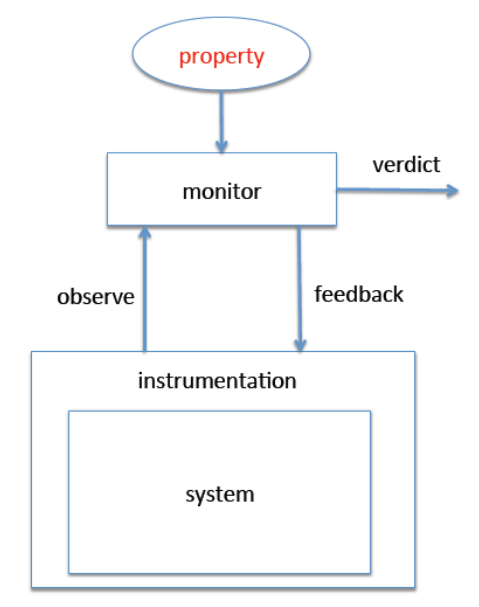
\includegraphics[width=80mm]{rvstruct.png}
\caption{Runtime verification process (from \cite{falcone2013tutorial})}
\label{img:rvstruct}
\end{center}
\end{figure}

Figure \ref{img:rvstruct} describes the process of a typical runtime verification system which contains the following four steps \citep{falcone2013tutorial}:
\begin{enumerate}
\item \emph{Monitor synthesis}: A monitor is synthesized from a property.
\item \emph{System instrumentation}: Extra instruments are integrated with the system under scrutiny in order to generate the events for the \emph{monitor}.
\item \emph{Execution}: The system is executed and starts to generate events and send them to the monitor.
\item \emph{Analysis and response}: The monitor analyzes the collected events, emits a \emph{verdict} and sends additional information, i.e. \emph{feedback} to the system if necessary.
\end{enumerate}

Monitors can be classified into several modes from different aspects \citep{chen2007mop}:
\begin{itemize}
\item \emph{online/offline} depends on when the monitors and the system work. \emph{Online} if they work at the same time, and \emph{offline} if the monitors start to work after the termination of the execution of the system.
\item \emph{inline/outline} depends on where the monitors are executed. \emph{inline} if the monitors are embedded into the system and \emph{outline} if the monitors run all alone while receiving the event traces from the system by certain methods, e.g. via file system or wireless signal.
\item \emph{violation/validation} is determined by the specification of the verdict.
\end{itemize}

From the definitions of the modes, we can see that a monitor working in offline mode is also working in outline mode and the inline mode implies the online mode.

\subsection{Comparison with other techniques}

Comparing with model checking \citep{clarke1999model} which aims to verify finite state systems, the methods of generating monitors in runtime verification and generating automatas in model checking have similarities. However, whereas model checking deals mainly with infinite traces, runtime verification deals only with finite traces, i.e. the executions. For this reason, the monitors of runtime verification working in online monitoring mode have to be able to accept incremental traces.

Another important difference between model checking and runtime verification is that, unlike model checking which checks if all executions of a system satisfy a correctness property, runtime verification is interested only with whether existing an execution which belongs to a set of valid executions. Moreover, runtime verification only requires to analyze the observed events of a given system without having to watch its internal running information, but in model checking, the proper model of the system must be acknowledged in order to prepare every possible execution before running the system. \citep{leucker2009brief}

Software testing \citep{broy2005model} is another verification technique. It is a process of running a program with a finite set of input-output sequences which is also namely test suite. Comparing with runtime verification, test suites are defined directly, unlike properties of runtime verification which are generated from formalism specification. Besides, ``exhaustive testing'' which is a common method in software testing, is normally not an option of runtime verification.

\section{Linear temporal logics}

In runtime verification, a monitor is translated from a correctness property, and correctness properties are specified in linear-time temporal logics, such as LTL.

Temporal logic is an extension of classical logic, and it provides a convenient language with the expressions of the properties to reason about the change of the states in terms of time. Although there are a lot of different temporal logics invented to meet various requirements, the temporal logics are normally classified by whether the time is linear or branching. The temporal logic with linear time is called \emph{Linear Temporal Logic} (LTL) which was first proposed by \cite{pnueli97}. Time in LTL is turned into a sequence of states which extend to the infinite future. The sequence of states is a computation \emph{path}. \citep{clarke1999model} \citep{huth2004}

\cite{leucker2009brief} summarizes LTL as a well-accepted linear-time temporal logic used to specify properties of infinite traces. However, in runtime verification, LTL is employed to check finite executions.

\subsection{Syntax}

A well-formed \emph{LTL} formula consists of a finite set of atomic propositions, boolean operators $\neg, \wedge, \vee, \rightarrow$ and temporal logic operators \textbf{F}(future), \textbf{G}(global), \textbf{X}(next), \textbf{U}(until), \textbf{W}(weak-until) and \textbf{R}(release). It can be represented in the Backus Naur form as follows \citep{huth2004}:
\begin{align}
\phi ::= & \top | \bot | p | (\neg\phi) | (\phi \wedge \phi) | (\phi \vee \phi) | (\phi \rightarrow \phi) \nonumber \\
& | (\X \phi) | (\F \phi) | (\G \phi) | (\phi \U \phi) | (\phi \W \phi) | (\phi \R \phi)
\end{align}

\subsection{Semantics}

For a sequence of states $s_0, s_1, s_2, ..., s_i, s_{i + 1}, ...$ where $s_{i + 1}$ is a future state of $s_i$, we define a path with $\pi^i = s_i \rightarrow s_{i + 1} \rightarrow ...$ where $i$ is the first state in this path. Given that $\pi(i)$ is the set of atomic propositions which are true at the $i$th state, whether a path $\pi^i$ satisfies an \emph{LTL} formula is defined as follows \citep{rozier2011linear}:

\begin{itemize}
  \item \listequation{\pi^i \vDash \top} \label{eq:true}
  \item \listequation{\pi^i \nvDash \bot} \label{eq:false}
  \item \listequation{\pi^i \vDash p \iff p \in \pi(i)} \label{eq:ap}
  \item \listequation{\pi^i \vDash \neg\psi \iff \pi^i \nvDash \psi} \label{eq:not}
  \item \listequation{\pi^i \vDash \psi \wedge \varphi \iff \pi^i \vDash \psi \text{ and } \pi^i \vDash \varphi} \label{eq:and}
  \item \listequation{\pi^i \vDash \psi \vee \varphi \iff \pi^i \vDash \psi \text{ or } \pi^i \vDash \varphi} \label{eq:or}
  \item \listequation{\pi^i \vDash \psi \rightarrow \varphi \iff \pi^i \vDash \varphi \text{ whenever } \pi^i \vDash \psi} \label{eq:then}
  \item \listequation{\pi^i \vDash \X \psi \iff \pi^{i + 1} \vDash \psi} \label{eq:next}
  \item \listequation{\pi^i \vDash \G \psi \iff \forall j \geq i, \pi^j \vDash \psi} \label{eq:global}
  \item \listequation{\pi^i \vDash \F \psi \iff \exists j \geq i, \pi^j \vDash \psi} \label{eq:future}
  \item \listequation{\pi^i \vDash \psi \U \varphi \iff \exists j \geq i, \pi^j \vDash \varphi$ and $\forall k, i \leq k < j, \pi^k \vDash \psi} \label{eq:until}
  \item \listequation{\pi^i \vDash \psi \W \varphi \iff$ either $\exists j \geq i, \pi^j \vDash \varphi$ and $\forall k, i \leq k < j, \pi^k \vDash \psi$, or $\forall k \geq i, \pi^k \vDash \psi} \label{eq:wuntil}
  \item \listequation{\pi^i \vDash \psi \R \varphi \iff$ either $\exists j \geq i, \pi^j \vDash \psi$ and $\forall k, i \leq k \leq j, \pi^k \vDash \varphi$, or $\forall k \geq i, \pi^k \vDash \varphi} \label{eq:release}
\end{itemize}

Formul\ae{}s \ref{eq:true} and \ref{eq:false} suggest that the states in the path $\pi^i$ should be always true or false.

In formul\ae{} \ref{eq:ap}, $p$ is an atomic proposition belonging to the finite set of atomic propositions of LTL, and this formul\ae{} demands to check only the $i$th state.

Formul\ae{}s \ref{eq:not}---\ref{eq:then} are boolean operators of propositional logic following the rules of Table \ref{table:prologic}

\begin{table}[h]
\centering
\begin{tabular}{|c|c|c|c|c|c|}
\hline
$\psi$ & $\varphi$ & $\neg\psi$ & $\psi \wedge \varphi$ & $\psi \vee \varphi$ & $\psi \rightarrow \varphi$ \\
\hline
True & True & False & True & True & True \\
\hline
True & False & False & False & True & False \\
\hline
False & True & True & False & True & True \\
\hline
False & False & True & False & True & True \\
\hline
\end{tabular}
\caption{The truth table of boolean operators of propositional logic}
\label{table:prologic}
\end{table}

Formul\ae{}s \ref{eq:next}, \ref{eq:future} and \ref{eq:global} are unary temporal logic connectives.
\X means ``next time'' and it skips the $i$th state and evaluates the path $\pi^{i+1}$. \F stands for ``sometimes in the future'' which requires that from the $i$th state, a property holds in a future state on the path. And \G (``globally'' or ``always'') denotes that a property should hold on the every state from the $i$th state until the end or the infinite future.

Formul\ae{}s \ref{eq:until}, \ref{eq:wuntil} and \ref{eq:release} are binary temporal logic operators. \U is the abbreviation of ``until''. The formul\ae{} $\psi \U \varphi$ holds if $\varphi$ holds at a future state on the path, and before this state the property $\psi$ holds at every state. \W, ``weak-until'', is a weak version of \U, except that for the formul\ae{} $\psi \W \varphi$, $\varphi$ does not have to hold eventually in some future state. \R, which stands for ``release'', is actually a logic dual of \U, i.e. $\psi \U \varphi \equiv \neg(\neg\psi \R \neg\varphi)$. \R requires that for the formul\ae{} $\psi \R \varphi$, the property $\varphi$ should hold continuously until $psi$ holds or $psi$ does not hold eventually.

It is worth noting that in LTL, the two-valued logics might yield a premature result which is either true or false. As is mentioned above, LTL is defined to work with infinite traces whereas monitoring of runtime verification is only able to treat finite traces, which might lead to a conflict, especially in some running system. For instance, $\F \psi$ states that $\psi$ should hold in a future state. In a running system, as long as $\psi$ does not hold in the observed states, the results of the formul\ae{} are always $false$, but if $\psi$ holds in the next observation, the former results will become corrupted and obsolete. Therefore, \cite{bauer2006monitoring} proposed the three-valued logic LTL$_3$ which introduces an new value \emph{inconclusive} for the cases where the property cannot be evaluated immediately.

\subsection{Various LTLs}

\subsubsection{Metric Temporal Logic}

Metric Temporal Logic (MTL) \citep{chang1994compositional} was invented to reason about real-time properties. To precise time accurately, MTL cuts the time into numbered pieces which is also called timed transition modules, and employs boundary operators to constrain the temporal logic operators. Its formul\ae{} is defined as follows:
\begin{align*}
\phi ::= & \bot | p | (\phi \rightarrow \phi) | (\fullmoon_{\sim{}c}\phi) | (\circleddash_{\sim{}c}\phi) | (\phi \mathrel{U}_{\sim{}c} \phi) | (\phi \mathrel{S}_{\sim{}c} \phi) \\
& \mbox{where } \sim \in \{<, =, >, \equiv_d\} \mbox{ and } c \geq 0, d \geq 2
\end{align*}

$\fullmoon_{\sim{}c}\phi$ means ``Next'', $\circleddash_{\sim{}c}\phi$ means ``Previous'', $\phi \mathrel{U}_{\sim{}c} \phi$ means ``Until'' and $\phi \mathrel{S}_{\sim{}c} \phi$ means ``Since'' \citep{chang1994compositional}. Given that $T_i$ indicates the time of the $i$th state of the path $\pi^i$, whether a formul\ae{} holds at the position $j$ of the path $\pi$ is defined as follows (we ignore the propositional operators here):
\begin{eqnarray*}
\pi^i \vDash \fullmoon_{\sim{}c}\psi & \iff & \pi^{i+1} \vDash \psi \mbox{ and } T_{i+1} - T_i \sim c \\
\pi^i \vDash \circleddash_{\sim{}c}\psi & \iff & i \geq 1 \mbox{ and } \pi^{i-1} \vDash \psi \mbox{ and } T_i - T_{i-1} \sim c \\
\pi^i \vDash \psi \mathrel{U}_{\sim{}c} \varphi & \iff & \exists j \mbox{ where } i \leq j, \pi^j \vDash \varphi \mbox{ and } T_k - T_j \sim c, and \forall k \mbox{ where } i \leq k < j, \pi^k \vDash \psi \\
\pi^i \vDash \psi \mathrel{S}_{\sim{}c} \varphi & \iff & \exists j \mbox{ where } 0 \leq j \leq i, \pi^j \vDash \varphi \mbox{ and } T_j - T_k \sim c, and \forall k \mbox{ where } j < k \leq j, \pi^k \vDash \psi \\
\end{eqnarray*}

\subsubsection{Past time LTL}

Whereas LTL mentioned in the last part is defined to check the future states, Past time LTL (ptLTL) aims to verify the states in the past. A ptLTL formul\ae{} is defined as follows \citep{havelund2004efficient}:
\begin{align*}
\phi ::= & \top | \bot | p | (\neg\phi) | (\phi \wedge \phi) | (\phi \vee \phi) | (\phi \rightarrow \phi) \\
& | (\odot \phi) | (\diamond \phi) | (\boxdot \phi) | (\phi \mathrel{S_s} \phi) | (\phi \mathrel{S_w} \phi) \\
& | (\uparrow \phi) | (\downarrow \phi) | [\phi, \phi)_s | [\phi, \phi)_w
\end{align*}

As can be seen in the definition of the formul\ae{}, ptLTL keeps several basic operators as LTL and introduces five standard part time operators and four monitoring operators.

The five standard part time operators are $\odot $ which means ``previous'', $\diamond$ ``eventually in the past'', $\boxdot$ ``always in the past'', $\mathrel{S_s}$ ``strong since'' and $\mathrel{S_w}$ ``weak since''.

The monitoring operators $\uparrow \downarrow [,)_s [,)_w$ mean respectively ``start'', ``end'', ``strong  interval'' and ``weak  interval''.

The temporal operators' semantics are described as follows, in the same form of the last section:
\begin{eqnarray*}
\pi^i \vDash \odot \psi & \iff & \mbox{ if } i > 0, \pi^{i - 1} \vDash \psi, or \mbox{ if } i = 0, \pi^0 \vDash \psi \\
\pi^i \vDash \diamond \psi & \iff & i > 0 \mbox{ and } \exists j \mbox{ where } 0 \leq j \leq i, \pi^j \vDash \psi \\
\pi^i \vDash \boxdot \psi & \iff & i > 0 \mbox{ and } \forall j \mbox{ where } 0 \leq j \leq i, \pi^j \vDash \psi \\
\pi^i \vDash \psi \mathrel{S_s} \varphi & \iff & \exists 0 \leq j \leq i, \pi^j \vDash \varphi \mbox{ and } \forall k, j < k \leq i, \pi^k \vDash \psi \\
\pi^i \vDash \psi \mathrel{S_w} \varphi & \iff & \pi^i \vDash \psi \mathrel{S_s} \varphi \mbox{ or } \pi^i \vDash \boxdot\psi \\
\pi^i \vDash \uparrow \psi & \iff & \pi^i \vDash \psi \mbox{ and } \pi^{i - 1} \nvDash \psi \\
\pi^i \vDash \downarrow \psi & \iff & \pi^i \nvDash \psi \mbox{ and } \pi^{i - 1} \vDash \psi \\
\pi^i \vDash [\psi, \varphi)_s & \iff & \exists j \mbox{ where } 0 \leq j \leq i, \pi^j \vDash \psi, \mbox{ and } \forall k \mbox{ where } j \leq k \leq i, \pi^k \nvDash \varphi \\
\pi^i \vDash [\psi, \varphi)_w & \iff & \pi^i \vDash [\psi, \varphi)_s \mbox{ or } \pi^i \vDash \boxdot\neg\varphi \\
\end{eqnarray*}

\subsubsection{EAGLE}

EAGLE \citep{barringer2004rule} is a temporal finite trace monitoring logic supporting parameterized equations by combining minimal/maximal fix-point semantics with temporal operators.

Online runtime verification requires to accept incremental traces which means there are possible boundaries between traces. Minimal/maximal fix-point rules were designed to treat this problem. Before evaluating the next trace, the equations with maximal rules are required to be always right and the ones with minimal rules are only needed to be eventually right.

\section{Runtime verification frameworks}\label{sec:rv:frameworks}

In runtime verification, monitors are generated from formal specifications by runtime verification frameworks. There are four monitoring modes: offline, online, inline and outline as we discussed in the early part of this section. Many frameworks and systems using some variant or extension of LTL have been proposed, as Table \ref{table:rvframeworks} shows. 

\begin{table}[h]
\centering
\begin{tabular}{|c|c|c|}
\hline
Name & Logic & Mode \\
\hline
JPax\citep{havelund2001java} & LTL \& Past-time LTL & outline \\
\hline
JavaMaC\citep{kim2004java} & Past-time LTL & outline \\
\hline
Hawk \citep{d2005event} & Hawk & outline \\
\hline
Temporal Rover\citep{drusinsky2000temporal} & LTL \& MTL & outline \\
\hline
MOP \citep{chen2007mop} & Various & inline/outline/offline \\
\hline
\end{tabular}
\caption{Runtime Verification Frameworks}
\label{table:rvframeworks}
\end{table}

Java PathExplorer (JPaX) \citep{havelund2001java} is an online runtime verification system aiming to monitor the execution traces of Java program. It has three modules (shown in Figure \ref{img:jpax}): an instrumentation module, an observe module and an interconnection module. The program working with the instrumentation module sends necessary event traces to the interconnection module which then transmits the traces to the observe module possibly running on another computer. The instrumentation module is driven by a user-specified script written in Java or Maude which is applicable for the specification of runtime monitoring.

\begin{figure}[h]
\begin{center}
\centering
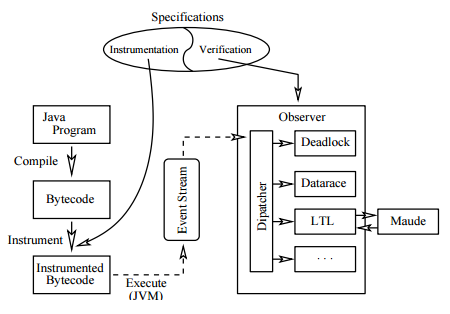
\includegraphics[width=100mm]{jpax.png}
\caption{JPaX Architecture (from \cite{havelund2001java})}
\label{img:jpax}
\end{center}
\end{figure}

JavaMaC \citep{kim2004java} is a ``run-time assurance system'' for Java programs while Mac means Monitoring and Checking. Its architecture is shown in Figure \ref{img:javamac}. Two definition languages are proposed: one for high-level specification which specifies required properties, another for low-level specification which defines the events and conditions. During the preparation, a ``filter'' and an ``event recognizer'' which are used to collect the necessary event traces are generated from the low-level specification, and a ``run-time checker'' is generated from the high-level spec. When running with the target program, events collected by the ``filter'' and ``event recognizer'' are sent to the ``run-time'' checker which is then responsible for the runtime verification work.

\begin{figure}[h]
\begin{center}
\centering
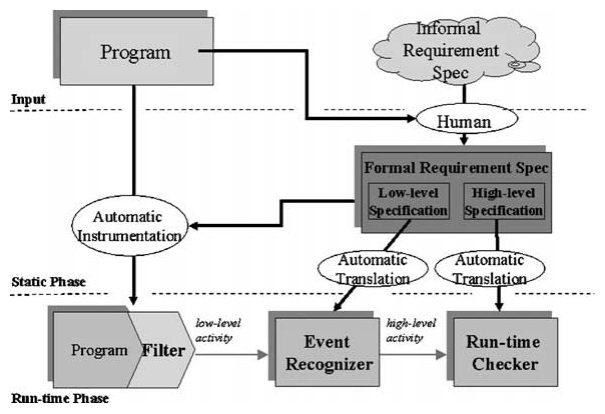
\includegraphics[width=100mm]{javamac.png}
\caption{MaC Architecture (from \cite{kim2004java})}
\label{img:javamac}
\end{center}
\end{figure}

\cite{d2005event} presents a logic named HAWK and its tools for RV of Java programs. HAWK is in fact built on EAGLE, another temporal logic which is considered more expressive \citep{barringer2004rule}. Although HAWK is event-based in contrast to state-based EAGLE, HAWK specifications are translated to EAGLE monitors. As Figure \ref{img:eagle} describes, during program execution, the EAGLE state is updated by instrumented program which then notifies the EAGLE observer. After that, the observer assesses the formul\ae{} in the current state to produce a result. 

\begin{figure}[h]
\begin{center}
\centering
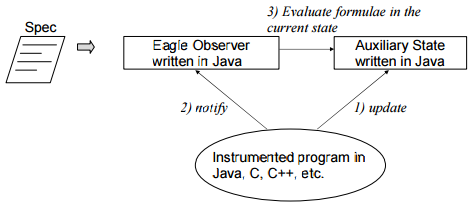
\includegraphics[width=100mm]{eagle.png}
\caption{Eagle Architecture (from \cite{d2005event})}
\label{img:eagle}
\end{center}
\end{figure}

Temporal Rover \citep{drusinsky2000temporal} is a commercial runtime verification tool based on LTL and MTL (Metric Temporal Logic). The specification code of Temporal Rover is inserted into the source code of Java, C, C++ or HDL and then converted into a compilable source file of corresponding language. A Temporal-Rover runtime verification system normally has two parts: host and target. The host is responsible for the verification while the target performs the computation of propositional formul\ae{} and sends back the results to the host via serial port, RPC or other customizable protocol.

Each of the frameworks discussed above hardwires a different specification formalism, which suggests that a general specification formalism serving all purposes does not exist. To be more expressive and generic, \cite{chen2007mop} introduced customizable and extensible ``logic-plugins'' in their runtime framework MOP and designed its architecture shown in Figure \ref{img:mop} with two layers: one is called ``language clients'' which support different programming languages, while another is ``logic repository'' which includes and manages various ``logic-plugins'' to support different specification formalisms, such as : Linear Temporal Logic (ltl), Finite State Machines (fsm), Extended Regular Expressions (ere), Context Free Grammars (cfg) and String Rewriting Systems (srs).

\begin{figure}[h]
\begin{center}
\centering
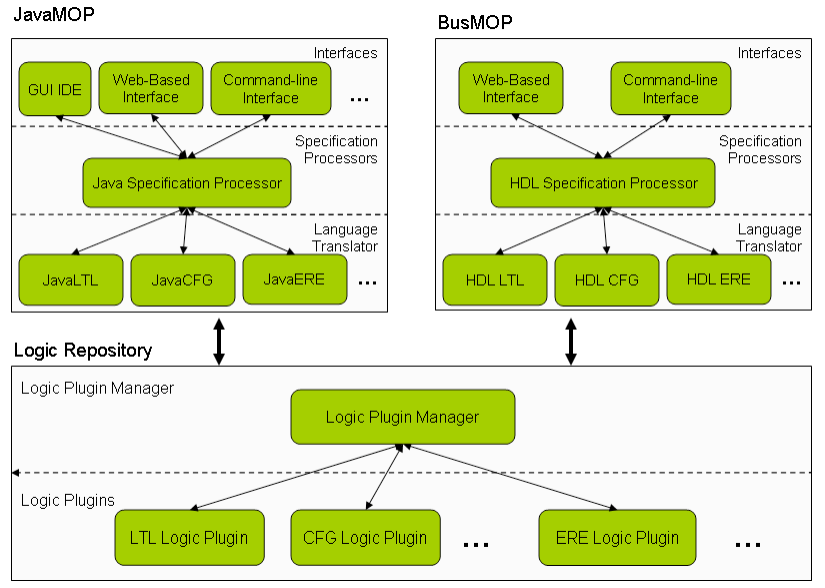
\includegraphics[width=130mm]{mop.png}
\caption{MOP Architecture (from \cite{chen2007mop})}
\label{img:mop}
\end{center}
\end{figure}

Besides the frameworks presented above, there are also lots of other frameworks invented for their corresponding requirements or specific temporal logics. Comparing these frameworks, we can find that they have their specialties as well as they share some common characters. For example, nearly all frameworks support online monitoring mode, Java programming language and network communication perhaps because these features are the most popular requirement in industry. Temporal Rover is a commercial RV framework, so it has to support more programming languages and supply more data collection options in order to expand its marketing. MOP was designed to be extremely general, resulting that most components can be changed or separately optimized.

%!TEX root = these.tex

\chapter{Communication en streaming et en temps réel avec les codes optiques}

Ce chapitre présente une version reformatée et traduite d'un article publié en 2016 dans IEEE Access, v.4, p.284-298 par K. Xie, S. Gaboury et S. Hallé.

%% -----------------------
%% Section: intro
%% -----------------------
\section{Introduction}\label{sec:qr:intro} %% {{{

La communication sans fil est une technologie qui permet à deux ou plusieurs pairs de communiquer sans câbles électriques ou conducteurs \citep{tse2005fundamentals}. Alors que la majorité des technologies de communication sans fil utilise les ondes radio comme leurs milieux de transmission, quelques autres utilisent la lumière, en particulier dans les situations où la technologie radio est difficile à fonctionner. La communication optique en elle-même remonte à l'utilisation de drapeaux, les signaux de fumée et les lampes signalétiques pour communiquer de l'information entre deux points avec l'utilisation d'un code spécifique \citep{burns2004}.

Récemment, une forme simple de communication optique, appelée \emph{Quick Response Code} (code QR) \citep{qrcode-about}, a émergé comme un raffinement de la technologie existante de code-barres unidimensionnels. En raison de leur exactitude et leur grande capacité, les codes QR ont été utilisés dans de nombreux domaines; les applications du traitement de tels codes ont également été portés à une variété de dispositifs, y compris les ordinateurs de bureau, les smartphones, et même les télévisions.

Cependant, jusqu'à présent les codes QR ont été utilisés pour la transmission de données statiques. En général, un code est imprimé sur un milieu physique, tel qu'une feuille de papier, et il est lu par un appareil optique (généralement une caméra) pour le décodage à un moment ultérieur. Dans ce chapitre, nous explorons l'idée de l'expansion de codes QR et les transformons en un canal dynamique de communication unidirectionnelle. Dans un tel canal, un flux de données est transmis par une \emph{séquence de codes}; généralement, ces codes sont continuellement générés et affichés sur un appareil, et simultanément capturés et décodés par un autre, ce qui est similaire aux autres types de technologies de communication.

Après avoir brièvement décrit dans la Section~\ref{sec:qr:reading} les bases de codes QR et d'autres technologies de communication sans fil, nous nous concentrons dans la Section~\ref{sec:qr:qrcode} sur le principe de communication de codes QR bruts. Particulièrement, nous essayons de trouver les limites intrinsèques d'un tel canal de communication, par l'analyse de l'influence de divers facteurs, tels que la densité de code, le nombre de codes affichés par seconde, etc. Les résultats d'un benchmark qui couvrent plus de cent combinaisons différentes de paramètres permettent d'extraire les conditions optimales qui minimisent le taux d'erreur dans le décodage des images, tout en maximisant la quantité de données qui peuvent être transmises par unité de temps.

Ces premiers résultats indiquent que les flux de codes QR peuvent en effet être utilisés comme un canal simple et unidirectionnel, mais que la communication sans erreur et la bande passante élevée sont plus ou moins impossibles. Par conséquent, en tant qu'un deuxième temps, nous concevons un protocole qui est approprié pour la nature spécifique de communication de codes QR. Ce protocole, appelé BufferTannen, est décrit dans la section~\ref{sec:qr:protocol}. Il est capable d'encapsuler les données brutes, de fournir diverses capacités de signalisation, de pouvoir représenter les données semi-structurées (telles que JSON) sous une forme binaire compacte, et prend en charge le cadrage/décadrage et le streaming de données.

Une seconde expérience révèle la robustesse de ce schéma de transmission: en utilisant notre protocole spécialement conçu, le canal de communication créé par une personne qui pointe un smartphone à bout de bras vers un écran avec les codes QR des codes QR vacillants, produit une bande passante suffisante pour transmettre l'audio à usage vocal en temps réel. La Section~\ref{sec:qr:experiments} présente l'environnement et les résultats des expériences de cette deuxième étape. Nous montrons aussi comment un morceau de données, coupé en plusieurs codes avec l'utilisation de BufferTannen, peut être reconstruit automatiquement par un utilisateur qui passe sa caméra sur une feuille de ces codes imprimés dans aucun ordre particulier.

Ce travail a été motivé par une application pratique dans le domaine de la vérification de l'exécution. Dans les recherches antérieures, nous avons proposé et officieusement expérimenté l'utilisation de codes optiques comme une forme de communication à couplage lâche entre un système logiciel et un moniteur externe qui reçoit les événements produits par ce système-là \citep{DBLP_conf/rv/LavoieLVGH14}. Dans ce contexte, la communication par les milieux optiques assure un isolement complet entre le système et son moniteur.

Bien que l'utilisation de séquences de codes QR a été officieusement suggéré dans le passé, au mieux de notre connaissance, notre recherche est la première enquête systématique du potentiel de codes QR pour envoyer les flux de données en temps réel.

La solution que nous proposons fournit une méthode pour distribuer les données en streaming sans dispositifs dédiés de communication. Les appareils requis sont seulement une caméra commune (comme une webcam ou la caméra dans un téléphone portable) et une petite surface plane pour afficher les codes QR séquentiels --- par exemple, un écran d'ordinateur, une télévision ou un smartphone, ou même une feuille de papier.
%% }}} --- Section

%% -----------------------
%% Section: comment on lit les codes QR
%% -----------------------
\section{Communications sans fil}\label{sec:qr:reading} %% {{{

Cette section rappelle quelques technologies communes de communication sans fil. Malgré leur popularité et leur performance, chacune a ses propres limites et ses scénarios d'application.

\subsection{Ondes Radio}

Le premier milieu évident de communication sans fil est grâce à l'utilisation d'ondes radio, dont le meilleur exemple est WiFi \citep{Comer:2008:CNI:1816918}, utilisé pour la mise en réseau sans fil de la zone locale. Ses variantes sont basées sur la famille de standards IEEE 802.11, et prennent en charge la mise en réseau centralisée (routage) et décentralisée (\textit{ad hoc}). Le Tableau \ref{tab:qr:wifi-protocol} montre les standards populaires de 802.11 et une partie de leurs spécifications.

\begin{table}[ht]
\begin{center}
\begin{tabular}{|c|c|c|c|}
\hline
Protocole &	Fréquence & Débit maximal de données physiques	&	Portée intérieure \\
\hline
802.11a &	5 GHz &	54 Mbps &	35 m \\
\hline
802.11b &	2.4 GHz &	11 Mbps &	35 m\\
\hline
802.11g &	2.4 GHz &	54 Mbps &	38 m\\
\hline
802.11n &	2.4/5 GHz &	150 Mbps &	70 m\\
\hline
802.11ac &	5 GHz &	866.7 Mbps & 35 m\\
\hline
\end{tabular}
\caption{Résumé des protocoles WiFi \citep{theng2008ubiquitous,perahia2013next}}
\label{tab:qr:wifi-protocol}
\end{center}
\end{table}

Un deuxième concurrent dans cette famille est Bluetooth \citep{Comer:2008:CNI:1816918}, qui est utilisé à courte portée et généralement comme communication point à point entre les appareils. Sa portée varie d'environ 1 à 100 mètres en fonction de la classe d'énergie. Le Tableau \ref{tab:qr:bluetooth} montre différentes versions de Bluetooth et leurs débits de données spécifiques.

\begin{table}[ht]
\begin{center}
\begin{tabular}{|l|r|c|}
\hline
Version &	Débit de données	&	Portée \\
\hline
Version 1.2 &	1 Mbps &	\multirow{4}{*}{\pbox{20\textwidth}{Classe 1: 100 m; \\ Classe 2: 10 m; \\ Classe 3: 1 m}}\\
\cline{1-2}
Version 2.0 + EDR &	3 Mbps & \\
\cline{1-2}
Version 3.0 + HS &	24 Mbps & \\
\cline{1-2}
Version 4.0 &	24 Mbps & \\
\hline
\end{tabular}
\caption{Spécifications de Bluetooth \citep{gupta2013inside}}
\label{tab:qr:bluetooth}
\end{center}
\end{table}

Enfin, ZigBee \citep {farahani2011zigbee}, basé sur le standard IEEE 802.15.4, vise à mettre en œuvre une communication sans fil à courte portée avec une faible énergie et une batterie de longue durée. Le Tableau \ref{tab:qr:zigbee} montre ses performances dans différentes bandes de fréquences.

\begin{table}[ht]
\begin{center}
\begin{tabular}{|l|r|c|}
\hline
Bande de fréquence & Débit de données	&	Portée \\
\hline
868--870 MHz &	20 kbps &	\multirow{3}{*}{\pbox{5 cm}{10--100 m, en fonction de la puissance de sortie et de l'environnement}}\\
\cline{1-2}
902--928 MHz &	40 kbps & \\
\cline{1-2}
2.4--2.4835 GHz  &	250 kbps & \\
\hline
\end{tabular}
\caption{Spécifications de ZigBee \citep{lee2007comparative}}
\label{tab:qr:zigbee}
\end{center}
\end{table}

Tous ces protocoles partagent un point commun: avant d'autoriser toute forme de communication entre deux extrémités, une certaine forme de \emph{découverte} ou \emph{configuration} de dispositifs est nécessaire. Ce processus est généralement achevé à travers l'établissement d'une \emph{connexion} avec états à long terme entre les extrémités.

\subsection{IrDA}

Dans une autre famille, on trouve des technologies utilisant des ondes infrarouges au lieu du signal radio \citep{sarkar2007ad}. Outre les longueurs d'onde différentes, ces technologies assouplissent généralement les exigences de l'établissement d'une connexion, et permettent une communication plus ``on-the-fly'' entre deux appareils. En règle générale, une extrémité d'une liaison infrarouge attend les données entrantes, tandis que périodiquement, un autre appareil pointe au récepteur et émet les rayons infrarouges transformés à partir de petits morceaux de données sans nécessité de préavis.

Une importance particulière est le standard IrDA (Infrared Data Association); ses émetteurs envoient des impulsions infrarouges avec un angle de cône et une irradiance modérée alors que ses récepteurs peuvent être à moins d'un mètre ou plusieurs mètres de ceux-là, en fonction de l'énergie des émetteurs et de la position dans le cône. La communication IrDA est semi-duplex et fournit CRC de base. Le Tableau \ref{tab:qr:irda-rate} montre plusieurs schémas IrDA et leurs débits de données dans la portée spécifique.

\begin{table}[ht]
\begin{center}
\begin{tabular}{|l|c|c|}
\hline
Schéma & Débit de données & Portée \\
\hline
SIR &	2.4--115.2 kbps &	\multirow{4}{*}{\pbox{3 cm}{jusqu'à un mètre}} \\
\cline{1-2}
MIR &	0.576--1.152 Mbps & \\ 
\cline{1-2}
FIR &	4 Mbps & \\
\cline{1-2}
GigaIR &	512 Mbps--1 Gbps & \\
\hline
\end{tabular}
\caption{Débits de données de schémas de couche physique de IrDA \citep{millar1998irda}}
\label{tab:qr:irda-rate}
\end{center}
\end{table}

\subsection{Visible Light Communication}

Comme l'indique son nom, Visible Light Communication (VLC) \citep{komine2004fundamental} utilise des longueurs d'onde dans la gamme visible (400-700 nm) pour communiquer les données entre les pairs --- ceci est généralement réalisé par allumer et fermer rapidement une source de lumière, ce qui permet une forme de codage des données comme les codes Morse. Un récepteur (par exemple une cellule photo-électrique) pointé par la source de lumière détecte ce vacillement et le convertit en données numériques. Avec les lampes fluorescentes comme la source lumineuse, le débit de données peut atteindre 10 kbps, tandis qu'avec la technologie LED, le débit de données peut être aussi élevé que 500 Mbps. La gamme dépend surtout des spécifications différentes, mais comme la lumière ne peut pas traverser les murs et peut également être affectée par le mauvais temps ou d'autres sources de lumière, sa portée et sa fiabilité sont limitées~\citep{arnon2015visible}.

Ce mode de communication est intrinsèquement unidirectionnel, car on ne peut pas répondre à la source de lumière, reconnaître la réception de l'information, ou demander d'une retransmission en cas de la perte de données. Par conséquent, cette technologie est aussi celle qui nécessite le moins de couplage entre un émetteur et un récepteur; selon tous les moyens pratiques, l'émetteur n'a pas connaissance de la présence d'un récepteur, qui, de son côté, peut choisir de commencer à recevoir à tout moment. Nous verrons plus loin que cette caractéristique est également partagée avec le canal de communication de codes QR que nous essayons de concevoir.

%% }}} --- Section

%% -----------------------
%% Section: le protocole
%% -----------------------
\section{Flux de codes QR}\label{sec:qr:qrcode} %% {{{

Dans le court sondage précédent de technologies de communication sans fil sont mentionnés les codes optiques, qui sont aussi un moyen de transport de données sans nécessité d'un milieu physique. Dans cette section, nous passons en revue le concept de codes QR, et discutons de l'idée de produire les flux de données par les séquences de tels codes.

\subsection{Aperçu de codes QR}

Un code QR (officiellement appelé ``Quick Response Code'') \citep{qrcode-about} est un code-barre à deux dimensions qui stocke des données, comme le montre la Figure \ref{fig:qr:helloqr}. En comparaison avec le code-barre bien connu UPC, qui est linéaire (i.e.\ unidimensionnel), un code QR peut stocker plus d'informations dans une impression plus petite.\footnote{\url{http://www.qrcode.com/en/}} Le standard du code QR stipule que ces codes peuvent avoir une capacité aussi élevée que 7089 caractères numériques ou 2953 caractères à 8 bits, et qu'un code est représenté dans un tableau carré d'un maximum de 177 $\times$ 177 ``pixels'', appelé \emph{modules} \citep{iso18004}.

\begin{figure}
\centering

\includegraphics[width=1in]{helloqr.png}
\caption{Un code QR avec le texte ``Hello world!''}
\label{fig:qr:helloqr}
\end{figure}

\begin{table}[t]
\begin{center}
\begin{tabular}{|c|c|c|c|c|c|}
\hline
Niveau de & Bits de & Caractère  & Caractère  & Caractère & Kanji \\
correction d'erreur & données & numérique & alphanumérique & binaire & \\
\hline
L &	23,648 & 7,089 & 4,296 & 2,953 & 1,817\\
\hline
M & 18,672 & 5,596 & 3,391 & 2,331 & 1,435\\
\hline
Q & 13,328 & 3,993 & 2,420 & 1,663 & 1,024\\
\hline
H & 10,208 & 3,057 & 1,852 & 1,273 & 784\\
\hline
\end{tabular}
\caption[Capacités]{Capacités maximales de stockage de codes de la version 40}
\label{tab:qr:qrcode-capacity}
\end{center}
\end{table}

La capacité d'un code QR dépend principalement de son type de données, de sa version et de son niveau de correction d'erreur. Le type de données peut être \emph {uniquement numérique}, \emph{alphanumérique}, \emph{binaire}, ou \emph{Kanji}. La version de 1 à 40, détermine les dimensions d'un code, qui varient de 21 $\times$ 21 à 177 $\times$ 177 modules. Les codes QR utilisent une forme de codage de correction d'erreur qui agit à quatre niveaux: \emph{Low} (L), \emph{Medium} (M), \emph{Quartile} (Q), et \emph{High} (H), comme il est indiqué dans le Tableau~\ref{tab:qr:qrcode-capacity}. Évidemment, comme le niveau augmente, plus de redondance est introduite dans le contenu du code, ce qui diminue sa capacité de stockage; cependant, plus de données peuvent être restaurées si le code est sale ou endommagé. Avec les formes de détection de position incluses dans le symbole, un code QR peut être décodé en 360 degrés.

Avant de générer un code QR à partir d'un morceau de données, un générateur de code doit analyser les données d'entrée pour décider du mode et de la version les plus efficaces. Dans le codage de données, les caractères sont convertis en un flux de bits, et dans ce progrès, certains \emph{indicateurs de mode} et \emph{terminateurs} sont insérés pour les changements de mode. Le flux de bits est ensuite divisé en mots de code à 8-bits, et les caractères de remplissage sont nécessaires pour combler le nombre de mots de code de la version choisie. La séquence de mots de code générée est divisée en blocs selon le niveau de correction d'erreur spécifique et un mot de code de correction d'erreur est généré pour chaque bloc. Ensuite, les mots de code de chaque bloc sont entrelacés et quelques bits restants sont ajoutés selon le besoin.

Dans l'étape suivante, le générateur met les modules de mots de code dans une matrice en noir et blanc avec la forme de recherche, les séparateurs, la forme de synchronisation et les formes d'alignement; il applique les formes de masquage, évalue et sélectionne ensuite la forme appropriée. Enfin, il génère le \emph{format} et \emph{l'information de version} et complète le code QR \citep{iso18004}.

Les étapes de décodage ne sont que tout simplement l'inverse de la procédure de codage. Dans un premier temps, le code QR doit être situé et les modules noirs et blancs sont reconnus comme 0s et 1s qui forment un tableau binaire. De ce tableau binaire, le décodeur reçoit l'information du format et de la version. Avec ces informations, il peut commencer à lire les caractères et les mots de code de correction d'erreurs, puis tente de détecter et de corriger les erreurs avec les mots de code de correction d'erreurs selon le niveau de correction d'erreur approprié. Dans l'étape suivante, les mots de code de données sont divisés selon le \emph{indicateurs de mode} et les \emph{indicateurs de nombre de caractères}, et les caractères de données sont finalement décodés et sortis.

\subsection{Le cas de communication de codes QR}

Le processus précité s'applique au codage et au décodage d'un code unique contenant des données statiques. Nous enquêtons maintenant sur l'idée d'utiliser les codes QR en tant qu'un canal de communication, où les données en temps réel seraient transformées en situation réelle comme une \emph{séquence} de codes QR, qui pourraient ensuite être optiquement capturées par un dispositif, et reconverties en flux de données d'origine à l'extrémité de réception.

L'utilisation de communication de codes QR présente plusieurs avantages dans une poignée de scénarios. Par exemple, la Marine américaine a enquêté sur l'utilisation de codes QR comme un ``sémaphore numérique''. La technologie proposée se concentre sur la détection de codes à basse résolution à partir de très longues distances, et souligne l'intérêt et les cas possibles d'utilisation de cette technologie dans un contexte militaire:

\begin{quote}
``Arguably the most significant advantage of QR code LOS [line of sight] communications is the fact that they can be conducted without emitting energy in the RF spectrum. In an emissions controlled (EMCON) environment, this will provide a critical ability to communicate between ships without increasing the possibility of position detection.'' \citep[p.\ 46]{richter-msc}
\end{quote}

Cependant, dans l'ouvrage cité, les codes sont considérés comme \emph{statiques}, c'est-à-dire qu'ils ne changent pas au fil du temps pour former un flux de données, et agissent plus ou moins comme un substitut de drapeaux ou de signes. Néanmoins, l'absence de toute émission d'ondes radio dans la communication de codes QR s'avère un avantage attrayant dans certains scénarios.

Nous avons également vu dans la section précédente comment toutes les autres technologies, telles que Bluetooth ou IrDA, nécessitent un matériel spécialisé. En revanche, la communication de codes QR peut être réalisée à travers les codes imprimés sur une surface dure, ou par un dispositif capable d'afficher des images à une résolution suffisante: les écrans de télévision, les écrans d'ordinateur, les tablettes et les téléphones cellulaires. De même, la réception peut être faite par un appareil équipé d'une caméra commerciale normale. Cela peut convertir les appareils équipés de ce matériel courant en dispositifs de communication, même s'ils ne sont pas conçus à cet effet en premier lieu. On peut même imaginer les situations d'urgence dans lesquelles tous les moyens numériques de communication entre deux points ne fonctionnent pas. Si la ligne de vision peut être établie et un affichage et une caméra sont disponibles, l'utilisation de codes QR permet néanmoins de transmettre les données numériques --- sans doute beaucoup plus rapidement que le manuel écriture ou transcription.

Enfin, nous avons mentionné au début comment l'utilisation d'un canal de communication optique et strictement unidirectionnelle peut également être souhaitable, même dans les situations où la communication radio ou câble est disponible. Par exemple, dans le contexte de la vérification de l'exécution, l'exécution d'un système est actuellement observée par un processus externe appelé \emph{moniteur}. Pour empêcher le moniteur d'interférer avec l'exécution du système, il est souvent placé sur une machine séparée, avec un canal de communication qui transporte les événements du premier au second. Cependant, dans les protocoles traditionnels tels que TCP, la nature bidirectionnelle d'une connexion présente un risque trop élevé d'attaques contre le programme de monitoring. En outre, certaines configurations de logiciels sont nécessaires pour brancher le moniteur au programme: les adresses IP, les noms de tube, les ports, etc., ce qui représente trop de couplage dans de nombreux scénarios. Nous avons discuté dans le travail précédent \citep{DBLP_conf/rv/LavoieLVGH14} comment l'utilisation d'un canal de communication optique peut atténuer ces problèmes en fournissant un plus grand isolement entre le système et son moniteur.

\subsection{Estimation de la bande passante et du taux d'erreur}

Cependant, la transmission unidirectionnelle introduit la possibilité de perte d'images pendant le procédure, en raison de la limitation des dispositifs physiques ou la vulnérabilité du logiciel. De plus, c'est impossible que l'émetteur puisse être conscient d'images manquantes à l'extrémité de réception et les renvoyer. Par conséquent, nous avons besoin d'analyser profondément cette approche pour estimer le \emph{taux de reconnaissance} et la \emph{bande passante de transmission} d'un tel canal de communication.

La transmission de codes utilise plusieurs paramètres: la taille de données de chaque image, le nombre d'images générées par seconde (fps) et le niveau de correction d'erreur. Tous les trois peuvent avoir un effet important de la génération de codes QR et de la bande passante résultante. Une plus grande taille de données mène à une plus haute version de symbole de codes QR et plus de modules de symboles, et avec la même taille d'image, un niveau plus élevé de correction exige plus de modules de symboles qu'un niveau moins élevé.

Comme l'émetteur ne peut pas détecter le fait que des codes soient manqués ou non par le récepteur, ce canal de communication unidirectionnel est en fait un canal avec perte, dont la bande passante actuelle peut être calculée avec le taux mesuré de reconnaissance d'images. Cela représente le nombre de bits qui sont reçus correctement.

\begin{equation*}
  bande\_passante = \mathit{fps} \times \mathit{bits\_de\_image} \times \mathit{taux\_de\_reconnaissance}
\end{equation*}

Si le récepteur craint que les images ne sont pas tout reçues, la seule façon est de s'assurer que l'émetteur envoie toutes les images plusieurs fois jusqu'à ce que le récepteur reçoit toutes les images; alors la bande passante réelle est la suivante:

\begin{equation*}
  bande\_passante = \mathit{fps} \times \mathit{bits\_de\_image} \div \mathit{nombre\_de\_fois\_de\_envoi}
\end{equation*}

Le taux de reconnaissance est normalement déterminé par la capacité de la caméra et de l'écran, la précision de l'algorithme de reconnaissance et la complexité de codes (c.-à-d. le nombre des modules affichés). Cependant, dans la capacité de la caméra et de l'écran, si nous pouvons envoyer la même image plus d'une fois, et entre-temps la valeur de \emph{fps} n'a pas à changer, le taux pratique de reconnaissance peut être amélioré.

\begin{equation*}
\mathit{taux\_pratique\_de\_reconnaissance} = 1 - (1 - \mathit{taux\_de\_reconnaissance})^{nombre\_de\_fois}
\end{equation*}


%% }}} --- Section

%% -----------------------
%% Section: expériences
%% -----------------------
\section{Expériences}\label{sec:qr:experiments} %% {{{

Dans cette section, nous décrivons les expériences où nous mesurons la précision de reconnaissance de séquences de codes QR dans diverses conditions. Le but de ces expériences est triple:

\begin{enumerate}
\item évaluer si les données peuvent être transmises avec succès à travers la reconnaissance de séquences de codes optiques;
\item trouver les paramètres qui maximisent la vitesse de décodage et la bande passante des données transmises;
\item à partir de ces résultats, déterminer les caractéristiques d'un canal typique de communication de flux de codes QR.
\end{enumerate}

\subsection{Préparation des expériences}

Notre installation expérimentale implique la production et l'affichage de séquences de codes QR à une extrémité, et la capture et le décodage de ces séquences à l'autre extrémité. Dans notre environnement expérimental, nous avons utilisé un écran LED de 19 pouces de Samsung comme émetteur et une webcam Logitech à haute définition comme récepteur. La caméra était mise à une distance fixe de 50 cm de l'écran. La résolution de l'écran est de 1280 $\times$ 1024 pixels.

La caméra était mise sur une surface stable, avec la zone de code optique correctement mise au point et couvrant tout le champ de vision. L'ordinateur utilisé dans les expériences est un ordinateur portable avec le processeur Intel Core i7-3632QM et 16 Go de mémoire. La Figure \ref{fig:qr:setup} montre l'installation utilisée dans les expériences.

\begin{figure}
\centering
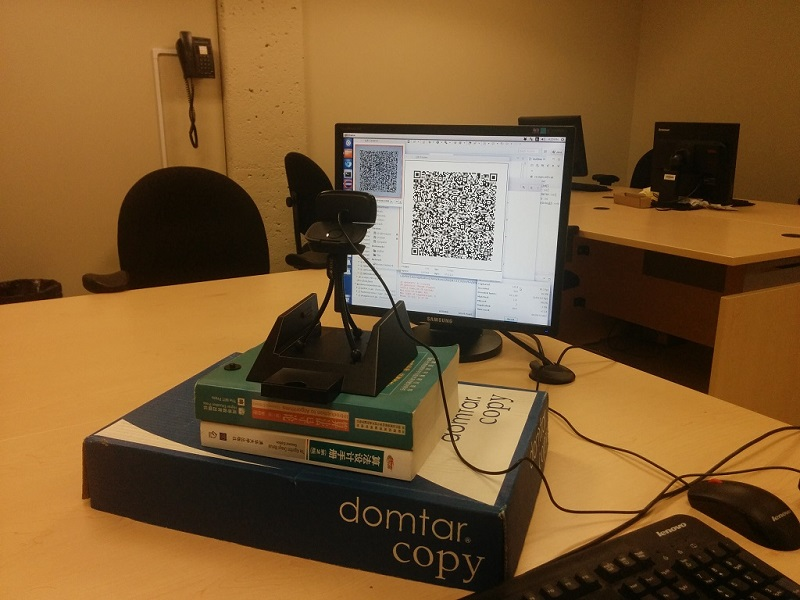
\includegraphics[width=\linewidth]{expsetup.jpg}
\caption{Installation expérimental pour lire les codes QR.}
\label{fig:qr:setup}
\end{figure}

Dans le développement, nous avons choisi OpenCV\footnote{\url{http://opencv.org/}} pour capturer les images de la caméra et ZXing\footnote{\url{https://github.com/zxing/zxing}} pour générer et décoder les codes QR. Pour réduire la pression du CPU et de la mémoire de capture et de décodage, les images capturées ont été transformées en 16 niveaux de gris. Les données utilisées pour générer les codes QR étaient les caractères alphanumériques aléatoirement générés. Tout le code du benchmark est implémenté en Java et disponible gratuitement.\footnote {\url{http://github.com/sylvainhalle/GyroGearloose}}

Le décodage de codes dépend de la qualité et de la complexité de l'image capturée. Si l'image est trouble ou cassée, elle sera difficile à décoder. Et les algorithmes de reconnaissance d'images peuvent avoir la probabilité de défaillance \citep{adel2006}. Par conséquent, notre première étape a pour but de mesurer la capacité des librairies de reconnaissance optique pour reconnaître correctement les séquences de codes, quelles que soient les données actuelles contenues dans ces codes. Les séquences de codes ont été générées par la production d'une chaîne de caractères de la forme \verb+dddd#rrrr...+, où \verb+dddd+ est un numéro séquentiel à partir de zéro et incrémenté par un dans chaque code successifs, et \verb+rrrr...+ est une chaîne de caractères aléatoires (différent dans chaque code) assez longue pour combler le code jusqu'à sa taille maximale. Chaque test consistait à filmer la séquence de tels codes et stocker le numéro séquentiel de chaque image correctement décodée dans un fichier. Cela nous permet de calculer la fraction de tous les codes qui ont été correctement reconnus; compte tenu de la taille de chaque code et du nombre de codes envoyés, cela permet de calculer la bande passante et le taux d'erreur de décodage.

Nos expériences ont rapidement trébuché par ce qui semble être un bogue dans de la librairie de décodage d'images ZXing. Lors de l'analyse de séquences d'images capturées par la caméra pour rechercher des erreurs de décodage, nous avons découvert que pour un nombre de fois, le décodage a échoué pendant que l'image correspondante semblait avoir aucun problème apparent (aucun trouble, cadrage juste, etc.). L'essai d'afficher encore les codes échoués à l'écran et puis d'essayer de les décoder avec la caméra n'a donné aucun succès, même après avoir changé la taille des codes, la position de la caméra, les conditions d'éclairage, etc. Le fait le plus curieux est que les codes immédiatement avant et après le code problématique ont été correctement décodées, tout en étant capturés dans les mêmes conditions. Même l'envoi de l'image ``pure''  du code directement à l'algorithme de décodage, sans aide de la caméra, produit une erreur de décodage.

Il semble donc la librairie ne peut pas reconnaître certains des codes qu'elle produit en soi (La Figure \ref{fig:qr:bad-code} montre un tel exemple). Cela indique très probablement un bogue de la librairie, qui a persisté jusqu'à la dernière version disponible au moment où ce chapitre a été écrit. Par conséquent, dans ce qui suit, le lecteur doit garder à l'esprit qu'une proportion inconnue d'erreurs de reconnaissance sont causées par ce soi-disant bug, et non par les conditions expérimentales particulières. Tel est le cas, par exemple, pour les écarts dans le taux de correction que nous observerons dans les Figures \ref{img-exp1}, \ref{img-exp2} et \ref{img-exp3}.

\begin{figure}
\centering

\includegraphics[width=.8\linewidth]{badqr.png}
\caption{Un code QR généré par ZXing que ZXing en soi ne peut pas décoder dans l'expérience.}
\label{fig:qr:bad-code}
\end{figure}

\subsection{Paramètres des expériences}

L'expérience vise à identifier la combinaison de paramètres qui permettraient de maximiser la bande passante et de minimiser le taux d'erreur de transmission de codes. Les paramètres qui ont été considérés sont les suivants.

\subsubsection{Résolution de codes}

Le premier paramètre est la taille de données de codes (c.-à-d. le nombre de bits de données contenues dans chaque code) et la taille physique (le nombre de pixels utilisés pour afficher le code sur l'écran). Nous avons varié la taille des données par incréments de 500 bits, de 500 à 4500 bits. Comme le montre le Tableau \ref{tab:qr:sample-sizes}, le plus grand code QR, qui contient 4500 bits de données en utilisant le niveau le plus élevé de correction d'erreur, occupe 101 $\times$ 101 modules. Nous avons aussi fixé la taille physique de codes à 700 $\times$ 700 pixels sur l'écran, ce qui rend chaque module un carré d'au moins 6 $\times$ 6 pixels.

\begin{table}[ht]
\begin{center}
\begin{tabular}{llll}
Nombre de bits & Niveau de correction & Version de symbole & Taille de symbole \\
de données d'entrées & d'erreur & & \\
\hline
\multirow{2}{*}{500} & L & 3 & 29$\times$29\\
& H & 5 & 37$\times$37\\
\hline
\multirow{2}{*}{1000} & L & 5 & 37$\times$37\\
& H & 9 & 53$\times$53\\
\hline
\multirow{2}{*}{1500} & L & 6 & 41$\times$41\\
& H & 11 & 61$\times$61\\
\hline
\multirow{2}{*}{2000} & L & 8 & 49$\times$49\\
& H & 13 & 69$\times$69\\
\hline
\multirow{2}{*}{2500} & L & 9 & 53$\times$53\\
& H & 15 & 77$\times$77\\
\hline
\multirow{2}{*}{3000} & L & 10 & 57$\times$57\\
& H & 17 & 85$\times$85\\
\hline
\multirow{2}{*}{3500} & L & 11 & 61$\times$61\\
& H & 18 & 89$\times$89\\
\hline
\multirow{2}{*}{4000} & L & 12 & 65$\times$65\\
& H & 20 & 97$\times$97\\
\hline
\multirow{2}{*}{4500} & L & 13 & 69$\times$69\\
& H & 21 & 101$\times$101\\
\hline
\multirow{2}{*}{5800} & L & 19 & 93$\times$93\\
& H & 30 & 137$\times$137\\
\hline\end{tabular}
\caption[Tailles d'échantillons]{Tailles d'échantillons de codes QR, selon leurs tailles de données et les niveaux de correction d'erreurs \citep{iso18004}}
\label{tab:qr:sample-sizes}
\end{center}
\end{table}

\subsubsection{Fréquence de codes}

Le deuxième paramètre expérimental que nous avons considéré est la fréquence de codes, c'est-à-dire le nombre de codes affichés par unité de temps. Nous avons d'abord choisi 2, 4, 6, 8 et 10 codes par seconde (cps), et également considéré jusqu'à 16 cps dans une phase ultérieure de l'expérience.

\subsubsection{Niveau de correction d'erreur}

Comme nous l'avons vu, les codes QR comprennent des données supplémentaires destinées à la correction d'erreurs. Nous avons donc aussi varié le niveau de correction d'erreur dans chaque expérience, en utilisant soit son réglage le plus élevé (H) ou le plus bas (L).

\subsubsection{Résolution et fréquence de la caméra}

La résolution de la caméra n'a pas été considérée comme un paramètre expérimental. Elle était fixe à sa valeur maximale, 1920 $\times$ 1080 pixels. De même, la fréquence d'image était fixe à 30 images par seconde. Cela correspond à la vidéo à haute définition 1080p, un réglage qui devrait être trouvé dans la plupart d'appareils récents et futurs de capture vidéo. Nous avons effectué quelques tests informels avec des basses résolutions (en baisse à 640 $\times$ 480), qui étaient mondialement concluants, mais qui n'ont pas été considérés pertinents de les inclure dans notre analyse détaillée.

\subsection{Résultats des expériences}

Le produit de toutes les combinaisons de tailles de codes, de niveaux d'erreur de correction et de fréquences de codes mène à un total de 90 expériences différentes. Ces expériences ont été répétées dans les trois ensembles, qui diffèrent par la façon dont les codes ont été affichés.

\subsubsection{Affichage en une fois}

Dans la première expérience, chaque code a été affiché en séquence pour une durée de $1/f$ seconde, où $f$ est la fréquence de codes. La bande passante et le taux de décodage sont présentés dans la Figure \ref{img-exp1} pour les combinaisons de tous les paramètres.

\begin{figure}
\begin{center}
\centering
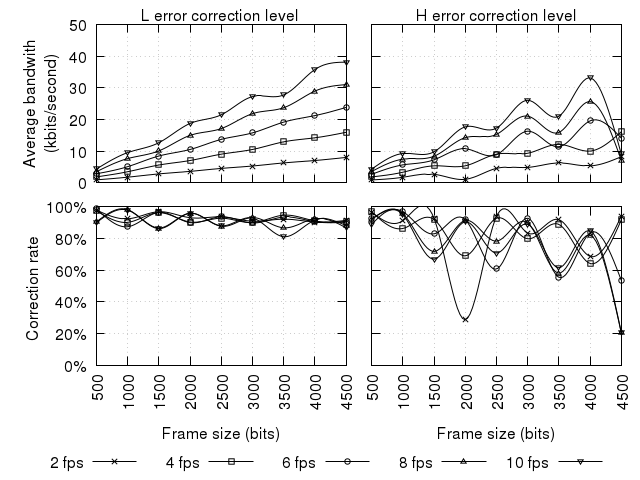
\includegraphics[width=\linewidth]{data1.png}
\caption{Bande passante et taux de décodage dans la première expérience}
\label{img-exp1}
\end{center}
\end{figure}

Comme on peut le voir, les taux de reconnaissance de niveaux plus élevé de correction étaient inférieurs à ceux de niveaux plus bas de correction, avec tous les autres paramètres étant égaux. Ceci peut être expliqué par le fait que la même quantité de données, portées dans un code avec un niveau plus élevé de correction, doit afficher plus de modules. Par exemple, selon le Tableau \ref{tab:qr:sample-sizes}, les modules d'un code 2000 bits en niveau H, sont aussi petits que ceux d'un code de 4500 bits en niveau L. Les modules plus petits, à leur tour, augmentent la difficulté de reconnaissance par la caméra. Par conséquent, une première conclusion que l'on peut tirer est que, de façon surprenante, la bande passante effective semble être améliorée en utilisant un bas niveau de correction d'erreur.

Avec les mêmes tailles de données et les mêmes niveaux de correction, la figure montre que le taux de reconnaissance diminue alors que la fréquence de codes augmente. Ceci peut être expliqué par le fait que, dans une fréquence plus élevée de codes, le même code occupe moins d'images de la caméra, et a donc moins de chances d'être correctement décodé dans l'une des images. En outre, la probabilité qu'un changement de code se produise au moment où une image soit prise (entraînant une image trouble qui montre une partie de deux différents codes) est également augmentée. En niveau L, la diminution est légère, tandis qu'en niveau H, la diminution est dramatique lorsque la taille du code atteint 3000 bits. Alors que la taille de données augmente, le taux de reconnaissance diminue constamment et considérablement.

Ces chiffres semblent indiquer que la configuration idéale pour le niveau L est 4500 bits et 10 fps, ce qui donne une bande passante effective de 39,0 kbps; pour le niveau H, 4000 bits et 10 fps mène à une bande passante de 24,6 kbps.

\subsubsection{Affichage en deux fois}

Considérant que la caméra pourrait avoir manqué plusieurs images, nous avons réalisé une seconde expérience dans laquelle chaque QR code est affiché deux fois dans une petite fenêtre du temps. Par conséquent, au lieu d'afficher chaque code une fois en $1/f$ seconde, chaque code a été entrelacé avec ses codes voisins et affiché deux fois en $1/2f$ seconde chaque fois. Ceci a pour résultat le même temps total d'exposition pour chaque code, mais augmente la diversité des images capturées par la caméra.

\begin{figure}[ht]
\begin{center}
\centering
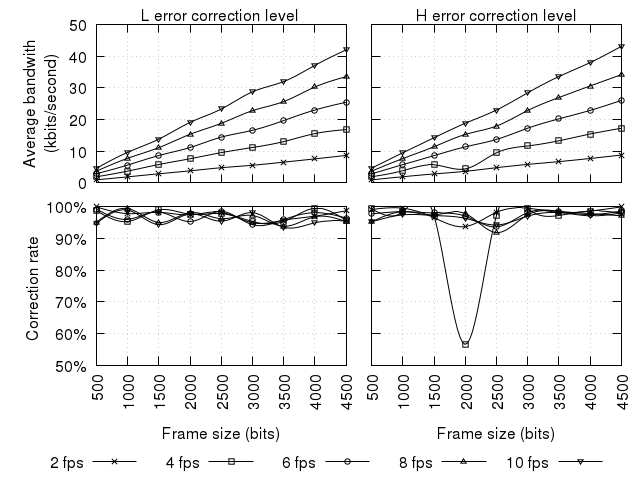
\includegraphics[width=\linewidth]{data2.png}
\caption{Bande passante et taux de décodage dans la deuxième expérience, où chaque code est affiché deux fois}
\label{img-exp2}
\end{center}
\end{figure}

Les résultats sont tracés sur la Figure \ref{img-exp2}. Ils montrent une augmentation de tous les taux de reconnaissance, qui sont maintenant tous supérieurs à 90\%. Ceci, à son tour, augmente la bande passante effective; en utilisant les mêmes paramètres que ci-dessus, on peut obtenir une bande passante de 43,0 kbps en utilisant le niveau L, et 44,1 kbps en utilisant le niveau H.

\subsubsection{Bourrage aléatoire}

Cependant, comme nous avons discuté plus tôt, les codes QR ne sont pas tous créés égaux; Avec la même résolution et le même niveau de correction d'erreur, les résultats expérimentaux indiquent que certains codes semblent être plus difficiles à reconnaître que d'autres. Par conséquent, la simple répétition de la même image en plusieurs fois n'a aucun impact sur cette intrinsèque ``dureté''. Notre troisième expérience présente encore un autre mécanisme pour augmenter le taux de reconnaissance.

Cette fois, nous avons essayé de générer les codes à partir des mêmes données d'entrée différentes en ajoutant, à la fin des données, une petite chaîne de caractères aléatoires qui est destinée à changer chaque fois où le code doit être affiché. De ce fait, les mêmes données originales, si elles sont affichées deux fois, sont préfixées à un différent bourrage aléatoire chaque fois, ce qui donne un peu différent tableau de bits. Toutefois, en vertu du schéma de codage QR, même un petit changement à la fin d'un tableau produit une forme complètement différente de points dans le code QR généré. La Figure \ref{fig:qr:difcodes} montre un exemple de ce phénomène. Par conséquent, si un code est plus difficile à reconnaître, les mêmes données sont également affichées dans une forme largement différente de points, ce qui augmente les chances d'être correctement ramassées au moins une fois.

\begin{figure}
\centering

\includegraphics[width=1in]{abcdefg.jpg}~
\includegraphics[width=1in]{abcdeff.jpg}
\caption{Exemples de deux codes avec les données légèrement différentes, mais avec de très différentes formes de points. Le code à gauche contient la chaîne ``abcdefg'', tandis que celui à droite contient ``abcdefg''.}
\label{fig:qr:difcodes}
\end{figure}

Bien que la raison objective que certains codes sont plus difficiles à reconnaître soit inconnue et hors sujet de ce chapitre, les résultats expérimentaux semblent confirmer cette hypothèse. Nous avons effectué une troisième expérience où chaque donnée d'entrée a été affichée trois fois avec différents codes QR générés. Le taux de reconnaissance est meilleure qu'avant lorsque la fréquence de codes est inférieure à 10 fps, comme le montre la Figure \ref{img-exp3}.

\begin{figure}[ht]
\begin{center}
\centering
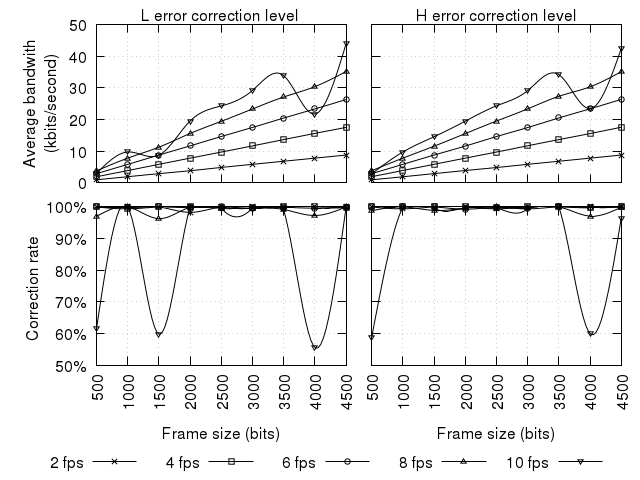
\includegraphics[width=\linewidth]{data3.png}
\caption{Troisième expérience: affichage en trois fois avec bourrage aléatoire}
\label{img-exp3}
\end{center}
\end{figure}

Ces résultats nous ont amenés à expérimenter avec les fréquences plus élevées de codes; nous avons ajouté 12 cps, 14 cps et 16 cps. Les codes ont été affichés deux fois. Comme la figure \ref{img-exp4} le montre, la bande passante maximale du résultat est 65,5 kbps en niveau L, et 68,3 kbps en niveau H, en utilisant 16 cps et les codes de 4500 bits.

\begin{figure}[ht]
\begin{center}
\centering
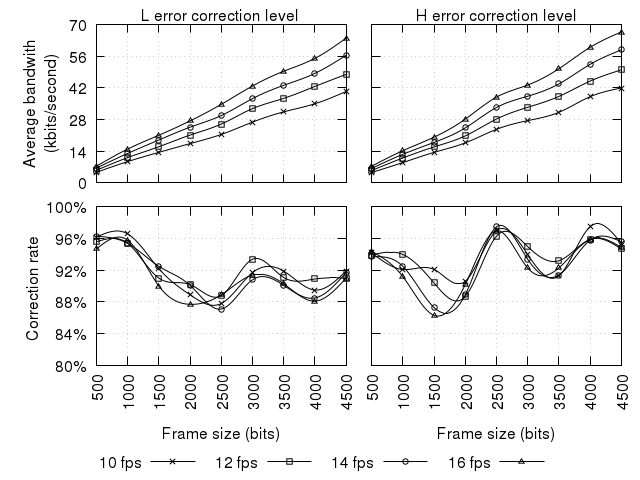
\includegraphics[width=\linewidth]{data4.png}
\caption{Quatrième expérience: affichage en deux fois et les fréquences plus élevées de codes}
\label{img-exp4}
\end{center}
\end{figure}

\subsection{Conclusions partielles}

Ces expériences initiales nous permettent de tirer quelques conclusions sur la nature d'un canal de communication de codes QR. Premièrement, bien que la fréquence plus élevée de codes et la taille plus élevée de codes aient un impact négatif sur le taux de reconnaissance, les données accrues qui peuvent être globalement portées compensent le taux plus élevé d'erreurs en termes de la bande passante effective. Deuxièmement, l'introduction de répétition et la variation de formes de points pour les mêmes données augmentent la bande passante effective; cela montre que deux codes différents pour la moitié du temps est plus efficace qu'un seul code pour le même intervalle. Troisièmement, même pour les plus petites tailles de codes, le taux d'erreur du canal est jamais zéro, ce qui indique que le canal est intrinsèquement avec perte.

A partir de ces constatations, on peut raisonnablement s'attendre qu'un flux de QR code fournisse un canal avec une bande passante effective d'environ 40 kbps, lors de l'affichage de 10 codes de 4000 bits par seconde en utilisant la technique de bourrage aléatoire et le niveau L de correction d'erreur. Le taux de décodage du canal avec ces paramètres doit être au moins 95\%. Évidement, ces constatations sont applicables à un réglage d'une caméra fixe. Elle ne prennent pas en considération la gigue potentielle, le flou ou d'autres effets qui peuvent se produire dans d'autres contextes ---bien qu'une expérience informelle décrite dans la Section \ref{subsub:swipe} tende à indiquer que la technologie est relativement robuste.

%% }}} --- Section

%% -----------------------
%% Section: le protocole
%% -----------------------
\section{Un protocole de canaux de communication unidirectionnelle avec perte}\label{sec:qr:protocol} %% {{{

Dans cette section, nous proposons une approche qui utilise les codes QR continus en tant qu moyen pour réaliser une transmission unidirectionnelle de données.

\subsection{Objectifs de la conception}

Afin de mettre en \oe{}uvre un canal de communication, un protocole spécifique est essentiel; il doit être bien conçu de telle sorte que les données peuvent être sérialisées et transférées sans coût important. En outre, le protocole doit avoir la capacité de diviser les données transférées dans des images pour générer les codes QR. Le résultat est BufferTannen, un logiciel Java dédié à la sérialisation et à la transmission de données structurées sur des canaux limités de communication.\footnote{\url{https://github.com/sylvainhalle/BufferTannen}} Il fournit un ensemble de classes permettant la représentation de données structurées sous une forme binaire compacte. Contrairement à d'autres systèmes, comme Protocol Buffers de Google\footnote{\url{https://github.com/google/protobuf}}, la définition de nouveaux types de messages peuvent être effectués lors de l'exécution et ne requiert pas la compilation de nouvelles classes utilisées. De plus, les messages dans BufferTannen ne peuvent pas être codés et décodés sans connaissance préalable de leur structure. Toutefois, étant donné que les messages ne contiennent pas d'information de leur structure, ils utilisent beaucoup moins d'espace.

BufferTannen définit aussi un protocole permettant la transmission de messages. Malgré que tout canal (e.g. connexion TCP, etc.) puisse être utilisé, BufferTannen a été conçu pour l'opération sur un canal avec les spécifications suivantes, qui sont basées sur nos premiers résultats expérimentaux:

\begin{itemize}
\item Le canal est point à point. Le but est d'envoyer de l'information directement de A à B; il ne fournit pas d'adressage, de routage, etc.
\item Le canal a une bande passante faible qui est en mesure de transmettre que quelques centaines d'octets à la fois, peut-être moins de 10 fois par seconde).
\item Le canal est unidirectionnel: généralement, un côté de la communication envoie des données qui doivent être ramassées par un récepteur. Cela implique que le récepteur ne peut pas détecter la réception de données ou demander à l'expéditeur de transmettre une autre fois, comme dans des protocoles, p.ex. TCP.
\item Le canal entraîne une perte. Cependant, nous supposons que le canal fournit un mécanisme (comme une forme de somme de contrôle) pour détecter et jeter des morceaux de données corrompues.
\item Un récepteur peut commencer à écouter sur le canal à tout moment, et être capable de recevoir correctement des messages à partir de ce moment-là. Ainsi, la communication n'a pas de ``début'' formel qui pourrait être appliqué, par exemple, pour annoncer des paramètres utilisés pour l'échange.
\end{itemize}

Par conséquent, le canal de communication envisagé comme le milieu de transmission pour les messages de BufferTannen peut être similaire, à bien des égards, à un signal de diffusion lente, comme Hellschreiber \citep{hells}, télévision à balayage lente \citep{slowtv}, Télétexte \citep{teletext} ou RBDS~\citep{rbds}.

Le protocole BufferTannen vise à transmettre des messages de manière aussi fiable que possible avec ces conditions, tout en préservant l'intégrité de données et l'ordonnancement de messages. La nature de la bande passante faible du canal explique l'accent de sérialisation de messages sous une forme binaire compacte. Puisque le récepteur ne peut pas demander de aucune forme de re-transmission, le protocole doit fournir le mécanisme qui retransmet automatiquement les messages afin de maximiser leurs chances d'être ramassés, alors qu'en même temps il ne doit pas confondre une re-transmission avec un nouveau message ayant un contenu identique. En outre, parce que le récepteur peut commencer à écouter à tout moment, et que le schéma de messages doit être connu afin de les décoder, les schémas de la communication doivent également être transmis à intervalles périodiques.

\subsection{Schémas}
\setcounter{paragraph}{0}

La déclaration d'une structure de données est appelée \emph{schéma}. L'information peut être représentée sous trois formes différentes:

\begin{itemize}
\item Smallscii: Une chaîne de caractères de longueur variable. Puisque BufferTannen vise à limiter autant que possible le nombre de bits requis pour représenter de l'information, ces chaînes sont restreintes à un sous-ensemble de 63 caractères ASCII (lettres, chiffres et ponctuations). Chaque caractère dans une chaîne Smallscii occupe 6 bits, et chaque chaîne se termine avec la chaîne de 6-bit \verb+000000+.

\item Integer: Le seul type numérique disponible en BufferTannen. Lorsqu'il est déclaré, les entiers, il leur est donné une ``largeur'', c.-à-d. le nombre de bits utilisés pour encoder. La largeur peut être une valeur entre 1 et 16 bits.

\item Enum: Une liste de constantes prédéfinies de Smallscii. Une énumération est applicable pour réduire davantage la quantité d'espace occupé par un élément de données lorsque son ensemble de valeurs possibles est connu à l'avance.
\end{itemize}

Ces blocs de construction de base peuvent être utilisés pour écrire des schémas en les combinant avec l'aide de structures de données composées:

\begin{itemize}
\item List: une séquence d'éléments de longueur variable, qui doivent tous être du même type (ou schéma). Les éléments dans la liste sont accessibles par leur index, en commençant par l'index 0.
\item FixedMap: une table qui associe des chaînes à des valeurs. La structure est fixe et les chaînes de caractères exacts qui peuvent être utilisés en tant que clés doit être déclarée. Cependant, chaque clé peut être associée à une valeur de type différent.
\end{itemize}

Ces constructions peuvent être mélangées librement. Ce qui suit représente la déclaration d'un schéma de messages complexes:

\begin{verbatim}
FixedMap {
  "titre" : Smallscii,
  "prix" : Integer(5),
  "chapitres" : List [
     FixedMap {
       "nom" : Smallscii,
       "longueur" : Integer(8),
       "type" : Enum {"normal", "appendice"}
     }
  ]
}
\end{verbatim}

La structure de haut niveau pour ce message est un map (délimité par \verb+{+\dots\verb+}+). Ce map a trois clés: \verb+titre+, dont la valeur associée est une chaîne Smallscii, \verb+prix+, dont la valeur associée est un entier dans la gamme 0-32 (qui occupe 5 bits), et \verb+chapitres+, dont la valeur n'est pas un type primitif, mais est une liste en soi (délimitée par \verb+[+...\verb+]+). Chaque élément de cette liste est un map avec trois clés: une chaîne \verb+nom+, un entier \verb+longueur+, et une énumération \verb+type+ dont les valeurs possibles sont \verb+normal+ ou \verb+appendice+.

Les schémas peuvent être représentés dans une représentation binaire compacte et sans équivoque comme suit.

\paragraph{Integer} La déclaration d'un entier est encodée comme la séquence de bits suivants:
%
\begin{verbatim}
ttt wwwww ddddd s
\end{verbatim}

La séquence \verb+ttt+ représente le type d'élément, encodé sur 3 bits. Un entier contient la valeur décimale 6. La séquence de \verb+w+ indique la largeur de l'entier en bits. La largeur elle-même est encodée en 5 bits. La séquence de \verb+d+ indique la largeur de l'entier en bits, s'il est exprimé comme une valeur delta, c.-à-d. comme la différence par rapport à un entier d'un message précédent. La largeur elle-même est encodée en 5 bits. Le seul bit \verb+s+ est le signe drapeau. Si la valeur est 0, l'entier est non signé; si elle est 1, l'entier est signé. Notez que des entiers exprimés en valeurs delta sont toujours codés comme les entiers signés; par conséquent, ce drapeau s'applique uniquement aux entiers qui se produisent en tant que valeurs complètes.

\paragraph{Smallscii} La déclaration d'une chaîne Smallscii est simplement encodée comme trois bits représentant le type d'élément; une chaîne contient la valeur décimale 2.

\paragraph{Enum} Une énumération doit fournir la liste de toutes les valeurs possibles qu'elle peut prendre. Elle est formellement représentée comme suit:
%
\begin{verbatim}
ttt llll [ssssss ssssss ... 000000 ...
 ssssss ssssss ... 000000]
\end{verbatim}

Le type d'élément est la valeur décimale 1, et la séquence \verb+llll+ est le nombre d'éléments dans l'énumération, encodé sur 4 bits. Ce qui suit est une concaténation de chaînes Smallscii qui définissent les valeurs possibles de l'énumération. Chaque caractère est encodé sur 6 bits, et la fin d'une chaîne est signalée par la séquence de 6 bits \verb+000000+.

\paragraph{List} La déclaration d'une liste est la suivante:
%
\begin{verbatim}
ttt llllllll ...
\end{verbatim}

Le type d'élément est la valeur décimale 3; le 8-bit séquence \verb+llllllll+ définit le nombre maximal d'éléments dans la liste. Ce qui suit est la déclaration du type d'élément des éléments dans cette liste.

\paragraph{FixedMap} Le dernier type d'élément est le map fixe, déclaré comme suit:
%
\begin{verbatim}
ttt [ssssss ssssss ... 000000 ddd...]
\end{verbatim}

Le type d'élément est la valeur décimale 4; ce qui suit est une chaîne Smallscii qui définit le nom d'une clé, suivie par la déclaration du type d'élément pour cette clé; ceci est répété pour autant de clés que le map déclare.

\subsection{Messages}
\setcounter{paragraph}{0}

Un \emph{message} est une instance d'un schéma. Par exemple, ce qui suit est un message possible en respectant le schéma précédent:

\begin{verbatim}
{
  "titre" : "hello world",
  "prix" : 21,
  "chapitres" : [
    {
      "nom" : "chapitre 1",
      "longueur" : 3,
      "type" : "normal"
    },
    {
      "nom" : "chapitre 2",
      "longueur" : 7,
      "type" : "normal"
    },
    {
      "nom" : "conclusion",
      "longueur" : 2,
      "type" : "chapitre"
    }
  ]
}
\end{verbatim}

Le lecteur qui est familier avec JSON ou des notations similaires remarquera des fortes similitudes entre BufferTannen et ces langages. Effectivement, les éléments d'un message peuvent être interrogés en utilisant une syntaxe similaire à JavaScript. Par exemple, en supposant que \verb+m+ est un objet qui représente le message ci-dessus, la récupération de la longueur du deuxième chapitre serait écrite comme l'expression:

\begin{verbatim}
m[chapitres][1][longueur]
\end{verbatim}

Ceci amène la valeur \verb+chapitres+ de la structure de haut niveau (une liste), puis le deuxième élément de cette liste (index 1), puis la valeur \verb+longueur+ de l'élément de map correspondant.

Avec les schémas, les messages peuvent être représentés sous une forme binaire compacte.

\paragraph{Smallscii} Les chaînes sont représentées comme une séquence de caractères de 6 bits, terminée par la fin du délimiteur de chaîne \verb+000000+.

\paragraph{Integer} Les nombres sont représentés par la séquence de bits qui encode leur valeur, sans aucune séquence de terminaison: le nombre de bits à lire est dicté par la taille de l'entier, tel que spécifié par l'élément de schéma correspondant. Si l'entier est signé, le premier bit représente le signe (0 = positif, 1 = négatif) et le reste de la séquence représente la valeur absolue.

\paragraph{Enum} Une énumération est simplement fabriquée en bits de séquence correspondant à la valeur appropriée. Encore, le nombre de bits à lire est dicté par la taille de l'énumération, tel que spécifié dans le schéma du message à lire. Par exemple, si l'énumération définit 4 valeurs, alors 2 bits seront lus. La valeur numérique $i$ correspond à la $i$-ème chaîne déclarée dans l'énumération.

\paragraph{List} Une liste commence par 8 bits qui enregistrent le nombre d'éléments dans la liste. Le reste de la liste est la concaténation de la représentation binaire de chaque élément de la liste. Puisque le type de chaque élément et le nombre de ces éléments à lire sont tous deux connus, aucun délimiteur n'est nécessaire entre chaque élément ou à la fin de la liste.

\paragraph{Fixed Map} Le contenu d'un map fixe est simplement la concaténation de la représentation binaire de valeur de chaque map. La clé auquel chaque valeur est associée, et le type de valeur à lire, sont précisés dans le schéma du message à lire, et devraient apparaître exactement dans l'ordre où ils ont été déclarés. Cela nous évite de répéter les clés de maps dans chaque message.

\subsection{Lire et écrire des messages}

En BufferTannen, les deux schémas et des instances de schémas sont représentés par le même objet, appelé \verb+SchemaElement+. Un SchemaElement vide doit d'abord être instancié en utilisant certains schémas; cela peut être effectué soit par:

\begin{itemize}
\item Lire une chaîne de caractères formatée comme ci-dessus; soit par

\item Lire une chaîne binaire qui contient un codage du schéma. En effet, en BufferTannen les messages et les schémas peuvent être transmis sous une forme binaire sur un canal de communication, et une méthode est fournie pour exporter le schéma d'un message dans une séquence de bits.
\end{itemize}

Une fois qu'un SchemaElement vide est obtenu, il peut être rempli avec des données, encore de deux façons:

\begin{itemize}
\item Lire une chaîne de caractères formatée comme ci-dessus; ou

\item Lire une chaîne binaire qui contient un codage des données.
\end{itemize}

Il y a des méthodes similaires pour fonctionner en sens inverse, et pour \emph {écrire} le schéma ou le contenu de données d'un message comme une chaîne de caractères ou une chaîne binaire. De cette façon, les messages et les schémas peuvent être librement encodés/décodés en utilisant des chaînes de textes lisibles ou des chaînes binaires compactes.

Comme on peut le voir, pour lire ou écrire un message, il faut d'abord instancier un objet avec un schéma. En fait, l'essai de décodage d'un flux de données sans publicité du schéma sous-jacent provoquera une erreur, même si le flux contient correctement des données formatées. De même, l'essai de lecture de données qui utilise un  schéma avec un objet instancié avec un autre schéma provoquera également une erreur. En d'autres termes, aucune donnée ne peut être lue ou écrite sans connaissance du schéma correct.

Cela peut sembler restrictif, mais il permet BufferTannen d'optimiser fortement la représentation binaire de messages. En l'absence d'un schéma connu, chaque message aurait besoin de porter, en plus de ses données réelles, de l'information de sa propre structure.

En pratique, grâce à lui, les répétitions de la description de son schéma dans chaque message se trouvent toutes dans les données du message. Au contraire, si le schéma est connu, toutes ces informations de signalisation peuvent être jetées: lors de la réception d'une séquence de bits, un lecteur qui possède le schéma connaît exactement le nombre de bits à lire, les données qu'il représente et la position où les données sont placées dans le structure de message. Cela implique toutefois qu'un récepteur qui ne connaît pas le schéma à appliquer n'a aucune idée sur la façon de traiter une chaîne binaire.

Pour illustrer l'intérêt de BufferTannen comme un schéma de codage de messages, nous considérons l'exemple de transmettre de événements à partir d'un jeu vidéo à un moniteur externe.

\subsection{Segments}
\setcounter{paragraph}{0}

Les messages et les schémas sont encapsulés dans une structure appelée \emph{segment}. Un segment peut être de quatre types:

\paragraph{Segments de message} contiennent la représentation binaire d'un message, avec un numéro séquentiel (utilisé pour préserver l'ordre des messages reçus), ainsi que le numéro se référant au schéma qui doit être utilisé pour décoder le message. Un segment de message est constitué d'un en-tête structuré comme suit:

\begin{verbatim}
tt nnnnnnnnnnnn wwwwwwwwwwww ssss ...
\end{verbatim}

L'en-tête commence par deux bits décrivant le type du segment; un segment de message contient la valeur décimale 1. Les sections \verb+n+ et \verb+w+ décrivent le numéro séquentiel et la longueur totale du segment, qui sont tous deux encodées sur 12 bits. Les quatre bits de \verb+s+ fournissent le numéro de schéma dans la banque de schéma qui devrait être utilisée pour lire ce segment. Le reste du segment est composé d'un map, d'une liste, d'une chaîne Smallscii ou d'un nombre, dont la représentation binaire a été décrite ci-dessus.

\paragraph{Segments de schéma} contiennent la représentation binaire d'un schéma, qui est associé à un numéro. Plusieurs schémas peuvent être utilisés dans la même communication, donc une banque de schémas identifiés par leurs numéros est crée. Un segment de schéma consiste en un en-tête structuré comme suit:

\begin{verbatim}
tt nnnnnnnnnnnn ssss ...
\end{verbatim}

L'en-tête commence par deux bits décrivant le type du segment; un segment de schéma contient la valeur décimale 2. La section \verb+n+ décrit le numéro séquentiel du segment, et la section \verb+s+ donne le numéro du schéma dans la banque de schémas auquel ce segment devrait être attribué. Le reste du segment est constitué d'une chaîne binaire décrivant le schéma, dont la représentation a été décrite ci-dessus.

\paragraph{Segments de blob} sont destinés à transporter des données binaires brutes selon le protocole BufferTannen.

\paragraph{Segments deltas} contiennent la représentation binaire d'un message exprimé comme la différence (``delta'') entre ce message et le précédent utilisé comme référence. Les segments deltas sont utilisés pour comprimer davantage la représentation d'un message, dans le cas où les messages ne changent pas beaucoup pour un intervalle de temps.

\begin{verbatim}
tt nnnnnnnnnnnn wwwwwwwwwwww rrrrrrrrrrrr...
\end{verbatim}

L'en-tête commence par deux bits décrivant le type du segment; un segment delta contient la valeur décimale 1. Les sections \verb+n+ et \verb+w+ décrivent le numéro séquentiel et la longueur totale du segment, qui sont tous deux encodées sur 12 bits. La section \verb+r+ donne le numéro séquentiel d'un autre segment, en rapport avec laquelle le delta du segment actuel est exprimé. Ce qui suit est une chaîne binaire qui décrit le contenu de la ``différence'', et il doit être calculé par rapport à ce segment pour obtenir le contenu de l'actuel.

Le calcul du delta est récursivement effectué sur chaque élément des deux messages pour comparer dans l'ordre où ils se produisent. Chaque type d'élément est défini comme suit.

\begin{itemize}
\item Smallscii strings: si les chaînes correspondantes sont identiques, émettre le seul bit \verb+0+. Sinon, émettre le bit \verb+1+ qui est suivi par la chaîne Smallscii du message cible.

\item Integers: si les numéros correspondants sont identiques, émettre le seul bit \verb+0+. Dans le cas contraire, émettre le bit \verb+1+ suivi par la différence entre la source et le nombre entier cible.

\item Enumerations: si la valeur correspondante du type énuméré est la même, émettre le seul bit \verb+0+. Autrement, émettre le bit \verb+1+ suivi par la valeur de l'entier correspondant à l'index de la valeur dans le message cible.

\item Lists: si les deux listes ont les mêmes éléments dans le même ordre, émettre le seul bit \verb+0+. Sinon, émettre le bit \verb+1+ suivi par la représentation binaire de la liste des cibles.

\item FixedMaps: appliquer récursivement les règles précédentes pour chaque clé du map.
\end{itemize}

On peut voir que les segments delta appliquent uniquement une forme grossière de comparaison. Par exemple, on ne tente pas de détecter si les deux listes diffèrent par l'addition ou la suppression d'un élément; le contenu de la liste est retransmis en intégralité chaque fois qu'il n'est pas identique à l'original. Néanmoins, cette technique permet de réaliser des économies substantielles chaque fois qu'une partie d'une structure de données reste identique d'un message à l'autre.

\subsection{Images}
\setcounter{paragraph}{0}

Le canal de communication envoie des données binaires en unités appelées \emph{images}. Une image est simplement un ensemble de segments concaténés sous une forme binaire, précédés d'un en-tête contenant le numéro de version du protocole (actuellement ``1'') et la longueur (en bits) du contenu de l'image. Formellement, la structure binaire d'une image est la suivante:

\begin{verbatim}
vvvv nnnnnnnnnnnnnn ffff... ffff...
\end{verbatim}

La section \verb+v+ est constituée du numéro de version de 4 bits du protocole, suivi de 14 bits indiquant la longueur (en bits) de l'image. Chaque segment est ajouté directement à cet en-tête de 18 bits. Parce que l'en-tête de chaque segment contient sa propre longueur, aucune autre transformation n'est nécessaire pour décoder correctement les données de segment.

Lorsque de nombreux segments sont en attente d'être transmis, le protocole tente d'adapter autant de segments que possible (dans un ordre séquentiel) au sein de la taille maximale d'une image avant de l'envoyer. Cette taille maximale peut être modifiée pour correspondre aux spécificités du canal de communication qui est utilisé. Dans l'incarnation actuelle du protocole, les segments ne peuvent pas être fragmentés en plusieurs images. Ainsi, un segment ne peut pas dépasser la taille maximale d'une image.

Chaque image est ensuite convertie en un code QR, avec son contenu binaire base64-encodé comme le texte de codes. Ce code QR peut alors être reconnu sur le site de réception, converti en une séquence binaire, et analysé et transmis aux images, aux segments et aux messages à travers l'application des transformations inverses.

\subsection{Modes de streaming}
\setcounter{paragraph}{0}

BufferTannen est conçu avec deux modes d'envoi, respectivement appelés le mode ``Lake'' et le mode ``Stream''.

Le mode Lake est destiné à l'envoi d'une pièce finie de données, comme un fichier, ou une séquence de messages BufferTannen dont le contenu complet est connu à l'avance. Les données à envoyer sont divisées en un ensemble fini de segments, et toute la séquence de segments est émise à plusieurs reprises à travers des codes QR. Si des images sont manquantes ou mal décodées, la répétition infinie de tous les segments permet d'attraper les données manquantes à la boucle suivante. Finalement, les erreurs de décodage peuvent indiquer que les données doivent être lues pour plus d'une boucle avant qu'elles soient complètement reçues.

L'utilisation du mode Lake peut être détectée par des images transportant une valeur non nulle à leur champ d'en-tête de ``segments totaux''. Ainsi, un récepteur qui commence à lire à tout moment la séquence d'images sait combien de segments doivent au total être reçus, et la position relative de chaque segment dans les données pour être reconstruite. Cela rend le mode Lake un schéma de transmission optique de données relativement lente, mais très robuste.

En mode Stream, les données sont constamment lues en segments qui forment alors un flux d'images, et les images sont immédiatement envoyées. Le processus de lecture arrête seulement quand il n'y a plus de données à lire. Les images déjà envoyées sont supprimées de la mémoire, donc il n'y a aucun moyen de renvoyer les données à plusieurs reprises. Cependant, pour le bien de la cohérence des données, nous avons fait un tampon pour les clones des images envoyées, et après avoir envoyé une quantité spécifique d'images récupérées à partir des données originales, les images dans la mémoire tampon sont renvoyées à nouveau, puis enlevées de la mémoire tampon . Par conséquent, le mode Stream est destiné à envoyer des données en temps réel, généralement là où la perte de données est acceptable et la consistance peut être légèrement sacrifiée (par exemple audio ou vidéo).

\begin{figure*}
\centering
\begin{verbatim}
--------------------------------------------------------------------------
Sending mode:        lake
Buffer state:        [||>       ||:.::||:|||] 59% (130/219)
Progress:            0408/0000 (13.8 sec @30 fps)
Link quality:        22/30 [*******   ] (73%)  Global:   339/454 (74%)
Data stream index:   0
Resource ident.:     myfile.jpg
Processing rate:     35 ms/frame (27 fps)
--------------------------------------------------------------------------
\end{verbatim}
\caption{Une partie de l'interface texte du récepteur de codes QR qui fonctionne en mode Lake}
\label{fig:qr:lake-gui}
\end{figure*}

La Figure \ref{fig:qr:lake-gui} montre une partie de l'interface texte de notre mise en œuvre de récepteur de codes QR. L'interface montre que les images étant reçues sont en mode Lake. Le champ d'état de tampon indique la progression de la réception. Dans cet exemple, il montre que les segments 130 sur 219 ont été correctement reçus; la barre de texte à gauche indique à quelles parties de la séquence totale ces segments correspondent. Une section de la séquence qui n'a pas été reçue du tout est indiquée par un espace vide; les parties de plus en plus complètes de la séquence sont représentées respectivement par les symboles \verb+.+, \verb+:+ et \verb+|+. Le symbole \verb+>+ indique la position relative du dernier segment qui a été lu correctement.

Le champ ``Link quality" donne une indication en temps réel du taux de décodage. Il montre que 22 des 30 dernières images capturées par la caméra ont été correctement décodées, et que globalement, 339 images ont été décodées sur 454 images capturées. L'identifiant de ressource et l'index de flux de données, portés par chaque image, sont également affichés.

\subsection{Résultats expérimentaux}
\setcounter{paragraph}{0}

Les expériences de la Section \ref{sec:qr:experiments} ont confirmé notre intuition que les flux de codes optiques sont un canal de communication intrinsèquement peu fiable et à faible bande passante. La compacité du protocole BufferTannen peut être motivée par un exemple de la vérification de l'exécution. Un jeu vidéo particulier, appelé Pingus, a été instrumenté pour produire des événements qui contiennent l'état de chaque personnage dans le jeu. Le schéma de ces événements est illustré à la Figure \ref{fig:qr:pingus-schema}.

\subsubsection{Transfert de fichiers}

\begin{figure}
\centering
\begin{verbatim}
FixedMap {
  "pingus" : List [
    FixedMap [
      "id" : Integer(6),
      "x" : Integer(10),
      "y" : Integer(10),
      "velocity-x" : Integer(4),
      "velocity-y" : Integer(4),
      "state" : Enum {"floater",
         "basher", "builder",
         "athlete", "normal"}
    ]
  ]
}
\end{verbatim}
\caption{Le schéma d'événements produits par un jeu vidéo instrumenté.}
\label{fig:qr:pingus-schema}
\end{figure}

Un événement contient généralement des données pour 50 caractères, ainsi la structure map est répétée autant de fois. L'envoi d'un tel événement en format texte clair, sans aucun espace, prend environ 3750 octets. À un fréquence de 30 événements par seconde, il prend 879 kbps de bande passante pour transmettre le flux d'événements. Le même événement dans BufferTannen prend 1.856 bits, ou 232 octets. Cela divise par plus de 16 les exigences de bande passante pour envoyer un flux de ces événements, ce qui donne une bande passante de 54 kbps.\footnote{Envoi de la même chaîne de caractères en Gzip se rétrécit vers à 716 octets, ce qui rend la compression standard une alternative moins attrayante dans ce contexte.} Dès cet instant, les segments de delta peuvent être utilisés pour réduire davantage la bande passante du flux, et transmettre les événements restants en utilisant un peu plus de 100 octets chacun, qui consomme une bande passante d'environ 24 kbps. Nos expériences précédentes montrent que cela est dans la gamme de ce que l'on peut raisonnablement s'attendre à transmettre à travers les codes QR.

Nous avons ensuite testé la capacité du protocole BufferTannen pour atténuer ces défauts, à travers son utilisation de répétition et sa représentation binaire compacte \footnote{Une vidéo de BufferTannen en action est disponible en ligne: \url{https://www.youtube.com/watch?v=GSL0md0TlY8}}

Nous avons choisi d'encoder des données en codes de 4000 bits, qui, après l'encapsulation de BufferTannen, équivaut à un code QR d'environ 5800 bits. Avec la combinaison de 5800 bits et du niveau L de correction, selon le Tableau \ref{tab:qr:sample-sizes}, la taille de symboles est d'environ 93 $\times$ 93 qui est entre les combinaisons de 3500 bits, du niveau H et de 4000 bits, du niveau H. D'après le résultat de la dernière expérience, les combinaisons de 4000 bits, du niveau H et tous les fps ont un taux de plus 95\% de correction   qui est fiable. D'autre part, les fréquences de codage sont 4, 6, 8, 10, 12 images par seconde. Selon la dernière expérience, cette configuration est fiable et censée être capable de fournir, respectivement 23.2--69.6 kbps et 16.0--48.0 kbps de bande passante. Étant donné l'application pratique, nous avons choisi de transférer un fichier d'exemple dont la taille est de 37,656 octets, et nous avons effectué chaque expérience 20 fois.

Le résultat de l'expérience du mode Lake dans la Figure \ref{img-explake} montre que la meilleure valeur de fps est de 10, et dans ce cas, le fichier d'exemple avait besoin d'être transféré en moyenne 2,4 fois pour s'assurer que le récepteur pourra obtenir toutes les images. Le temps passé en moyenne est de 17,27 secondes, et la bande passante est donc environ 17,0 kbps.

\begin{figure}[ht]
\begin{center}
\centering
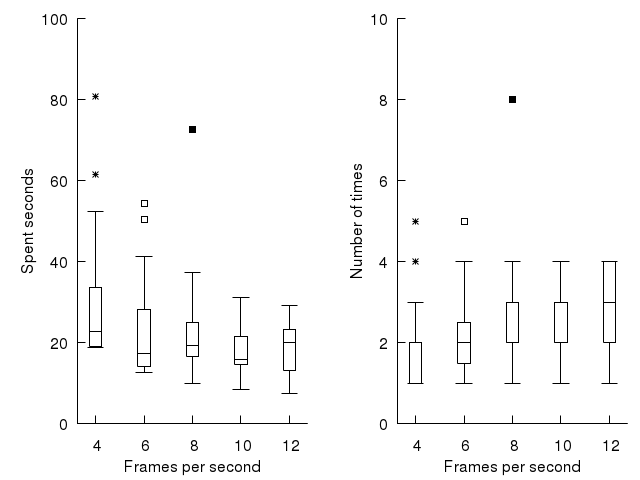
\includegraphics[width=\linewidth]{lake.png}
\caption{Temps de l'envoi des données en mode Lake}
\label{img-explake}
\end{center}
\end{figure}

En mode Stream, le pourcentage de codes reçus est important. Dans l'expérience, selon la Figure \ref{img-expstream}, les taux moyens d'achèvement de toutes les configurations sont plus de 99\%, et la configuration de 12 fps a besoin d'environ 13,11 secondes pour envoyer toutes les images avec un canal de streaming de données de 22,4 kbps .

\begin{figure}[ht]
\begin{center}
\centering
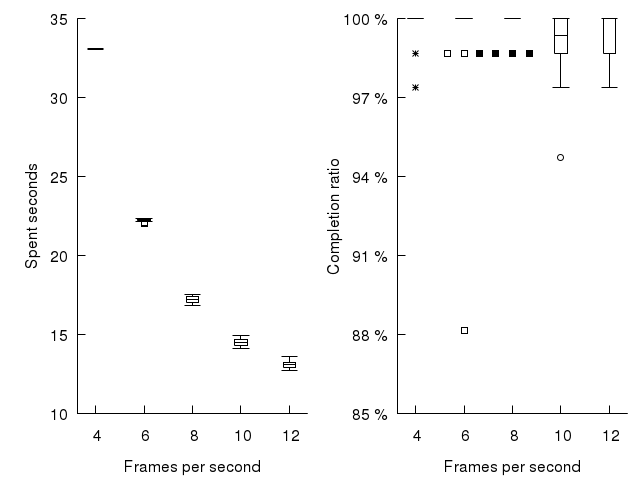
\includegraphics[width=\linewidth]{stream.png}
\caption{Temps de l'envoi des données en mode Lake Stream}
\label{img-expstream}
\end{center}
\end{figure}

\subsubsection{Glisser du papier}\label{subsub:swipe}

La capacité d'envoi des flux de données en mode Lake peut également être utilisée pour compléter la capacité intrinsèquement limitée de codes QR. Lors de l'affichage d'un code imprimé sur une feuille de papier, de grandes quantités de données peuvent être seulement apportées par l'augmentation de la résolution de codes; cependant, la résolution ne peut être augmentée jusqu'à une limite certaine et prédéfinie.\footnote{4296 caractères alphanumériques ou 3222 octets en codage Base-64.} En outre, pour des résolutions plus élevées, le code peut devenir difficile à reconnaître en utilisant des caméras en niveau d'entrée et en basse résolution. Par conséquent, c'est prudent de supposer que, avec l'aide de la technologie existante de codes QR, un maximum de  3000 octets de données peuvent être transférées à travers un code QR.

Cette limitation peut être surmontée par l'utilisation du protocole BufferTannen. Bien qu'aucun code dont la taille est supérieure à environ 4000 octets ne puisse être créé, plusieurs de ces codes peuvent être alignés sur un morceau de papier. Chacun de ces codes peut être formaté pour contenir une image unique de données envoyées par le protocole BufferTannen en mode Lake. Il suffit à l'utilisateur de glisser la caméra sur ces codes; en vertu du mode Lake, l'ordre dans lequel les codes sont scannés n'est pas pertinent, et les pièces complètes de données peuvent être correctement reconstruites à partir des images individuelles. c'est donc possible de théoriquement transmettre des quantités illimitées de données, tout en utilisant des codes d'une résolution inférieure (cette résolution inférieure étant compensée par la présence de plus d'un code).

Pour vérifier cette affirmation, nous avons imprimé sur une feuille de papier le contenu d'un fichier de 37 ko en tant qu'une séquence de codes QR, traités comme des images par BufferTannen en mode Lake. Nous avons ensuite passé la caméra au-dessus de cette feuille de papier à une distance d'une longueur de bras (montré dans la Figure \ref{fig:qr:paper-swipe}). L'interface utilisateur du logiciel affiche en temps réel le nombre d'images restantes à décoder et leurs positions dans le flux complet, qui donne à l'utilisateur des indications de codes que passe la caméra. Il convient de noter que la caméra fonctionnait en mode ``film'', et non en mode ``snapshot''. En d'autres termes, les images ont été capturées continuellement par la caméra lorsque elle était déplacée au-dessus de la feuille; l'utilisateur n'a pas besoin de pointer et de cliquer sur chaque code QR individuel (ce qui serait fastidieux).

\begin{figure}
\centering
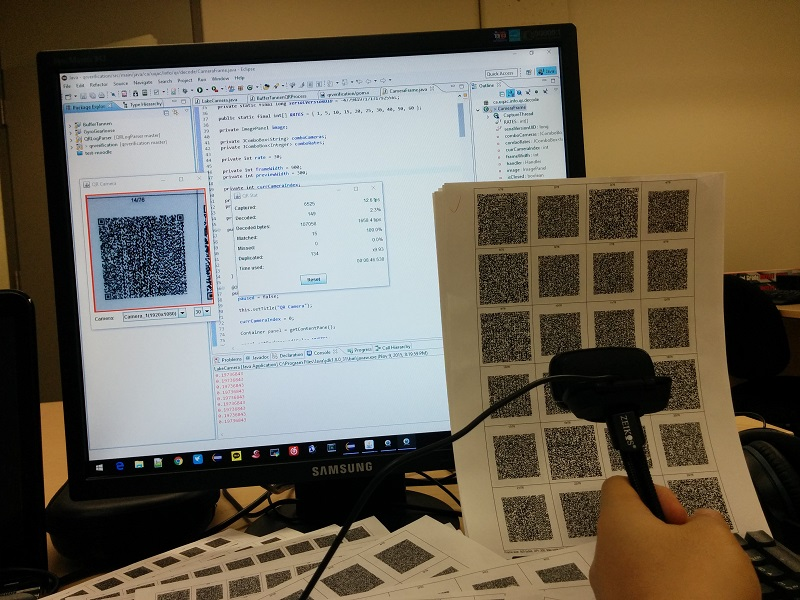
\includegraphics[width=\linewidth]{swipe.jpg}
\caption{Passer la caméra au-dessus d'un ensemble de codes QR pour reconstituer le contenu d'un fichier plus grand.}
\label{fig:qr:paper-swipe}
\end{figure}

Le niveau de correction d'erreur choisi était L et les tailles de données brutes par code que nous avons testées étaient 500, 750, 1000, 1250, 1500, 1750, et 2000 octets. Avec 500 octets, il y avait 76 codes tandis qu'avec 2000 octets, il y en avait seulement 19. Après avoir été encapsulées par le protocole BufferTannen, les tailles finales de données utilisées pour générer les codes QR sont devenues en conséquence 723, 1055, 1391, 1724, 2054, 2389 et 2722 octets. Les codes ont été imprimés à 300 ppp (points par pouces) et 600 ppp sur des papiers de bureau , et nous avons programmés pour donner 500 points à chaque bord de tous les codes dans le papier.

À 300 ppp, les codes dont la taille était de 500 à 1250 octets étaient tous décodés avec succès et en douceur. Cependant, quand la taille a atteint 1500 octets, le décodage est devenu plus problématique. Pour certains codes, nous avons dû recommencer plusieurs fois et coller la caméra près du papier pendant quelques secondes, mais parmi le total de 31 codes, trois restaient impossible à décoder. Dans le cas des codes de 1.750 et de 2.000 octets, aucun des codes n'aurait pu être décodé. Ceci peut être expliqué par le fait que les codes de densité plus élevée ont pour effet que chaque module de code est plus petit et ainsi plus difficile à capturer. Par exemple, le bord d'un code de 500-octets et du niveau L est d'environ 77 modules, de sorte que chaque module peut avoir environ 6 points dans le papier, tandis que le bord d'un code de 2000-octets et du niveau L est 149 modules, donc chaque module ne peut avoir que 3 points pour imprimer.

À 600 ppp, aucun des codes ne pourrait pu être décodé, peu importe le nombre d'octets qu'ils ont apporté. La raison en est que les codes imprimés à 600 ppp sont trop petits et la caméra doit approcher de très près au papier, mais les images capturées étaient toutes troubles et hors de foyer. Ceci semble donc que les codes imprimés à 600 ppp sont au-delà de la capacité d'une standard caméra web.

Néanmoins, cette expérience démontre la viabilité du concept de passer une caméra à travers un tableau de codes QR. Nos découvertes empiriques indiquent qu'un flux de données peut être divisé en un ensemble de codes QR d'environ 1000 octets chacun, dont le contenu correspond à des images individuelles du protocole BufferTannen qui contiennent les données de transmission. Il suffit de passer la caméra au-dessus de cet ensemble de codes, dans aucun ordre particulier, pour reconstruire le contenu complet de données du côté de l'appareil.

%% }}} --- Section

%% -----------------------
%% Section: Conclusion
%% -----------------------
\section{Conclusion}\label{sec:qr:conclusion} %% {{{

Dans ce chapitre, nous avons présenté une solution d'un canal de communication unidirectionnelle sur la base de codes QR, et réalisé des expériences pour mesurer sa performance. Nous avons d'abord testé expérimentalement les caractéristiques d'un flux de données de codes QR sous diverses conditions, et extrait les paramètres qui  maximisent la bande passante effective du canal. Toutefois, étant donné que le canal est intrinsèquement enclin à erreur et à faible bande passante, nous avons ensuite introduit BufferTannen, un protocole conçu spécialement pour ce type de canal. BufferTannen prend soin du fractionnement, de la transformation, et dans une certaine mesure avec la compression des données de transmission afin de maximiser l'efficacité du flux de codes QR. La faisabilité de cette approche a ensuite été empiriquement observée lors d'une nouvelle série d'expériences.

Même avec les limites du protocole et du canal de communication, les résultats présentés peuvent être utilisés à bon escient dans une variété de situations. Dans les environnements limités où l'utilisation du signal de radio ou de câbles est interdite ou difficile, notre approche peut fournir un moyen facile pour communiquer entre pairs, soit comme sauvegarde d'urgence ou comme moyen principal. Par ailleurs, en raison de l'évolution de la qualité des deux dispositifs d'affichage et de capture d'images, c'est possible de prévoir des vitesses de transmission accrues dans l'avenir.

Enfin, les techniques susmentionnées pourraient être transformées en une liaison de communication bidirectionnelle dans le cas de terminaux équipés d'une caméra et d'un écran. Dans un tel cas, les reconnaissances d'images correctement décodées pourraient être échangées, ce qui permettrait de renvoyer des données sur demande et d'augmenter la bande passante effective.

%% }}} --- Section
%!TEX root = these.tex

\chapter{Évaluation hors ligne de formules LTL avec les manipulations de bitmaps}

Ce chapitre présente une version modifiée et traduite d'un article qui est écrit par K. Xie et S. Hallé et qui est encore en cours de révision pour sa publication dans les actes de la conférence internationale: Runtime Verification 2016 (RV'16) à Madrid, Espagne en 2016.

%% ------------------
%% Section: intro
%% ------------------
\section{Introduction}\label{sec:bm:intro} %% {{{

Une \emph{logique temporelle} \citep{huth2004} est un système logistique qui utilise des règles et des symboles pour décrire et raisonner sur le changement de l'état d'un système en termes de temps. Elle est basée sur l'idée qu'un état ne peut pas rester constamment vrai ou faux avec le temps. Une \emph{Logique Temporelle Linéaire (LTL)} \citep{pnueli97} est une logique temporelle, et comme son nom l'implique, une \emph{LTL} peut désigner une seule séquence d'états et pour chaque état il n'y a qu'un état futur.

Un \emph{bitmap}, qui est également connu sous forme de tableau de bites ou de bitset, est une structure compacte de données stockant une séquence de valeurs binaires. Comme on le verra dans la section \ref{sec:bm:compression}, il peut être utilisé pour exprimer un ensemble de nombres, ou un tableau dont chaque bit représente une option de 2 valeurs. Les bitmaps présentent plusieurs avantages en tant qu'une structure de données: ils peuvent représenter brièvement de l'information et fournir des fonctions très efficaces pour les manipuler, grâce au fait que les bits multiples peuvent être traités en parallèle à travers une seule instruction du processeur.

Dans ce chapitre, nous explorons l'idée de l'utilisation des manipulations de bitmaps pour l'évaluation hors ligne de formules LTL d'un journal d'événements. A cet effet, dans la section \ref{sec:bm:ltlbitmap}, nous introduisons une solution qui, pour une trace d'événements données $\sigma$ et une formule LTL $\varphi$, convertit d'abord des termes de base en autant de bitmaps; intuitivement, le bitmap correspondant à une proposition atomique $p$ décrit les événements de $\sigma$ qui satisfont $p$. Les algorithmes sont ensuite détaillés pour chaque opérateur LTL qui prend des bitmaps comme leur entrée et qui retourne un bitmap comme leur sortie. L'application récursive de ces algorithmes peut être utilisée pour évaluer toute formule LTL.

Cette solution présente plusieurs avantages. Tout d'abord, l'utilisation de bitmaps peut être considérée comme une forme d'\emph{indexation} (dans le sens du terme de base de données) du contenu d'une trace. Plutôt que d'être un algorithme en ligne qui lit simplement une trace pré-enregistrée, notre solution exploite le fait que la trace est complètement connue à l'avance, et profite largement de cet indice pour accéder directement à des endroits spécifiques dans la trace afin d'accélérer son processus. Deuxièmement, un bitmap ayant des 0s ou 1s consécutifs peut être compressé, ce qui réduit le coût de l'espace et accélère profondément l'exécution de nombreuses opérations \citep{lemire2014}.

À cette fin, la Section \ref{sec:bm:experiments} décrit une installation expérimentale utilisée pour tester notre solution. Elle révèle que, pour des formules LTL complexes qui contiennent près de 20 opérateurs temporels et conjonctifs, des grandes traces d'événements peuvent être évaluées à un débit de plusieurs dizaines de millions d'événements par seconde. Ces expériences montrent que les bitmaps sont une structure de données compact et rapide, et sont particulièrement appropriés pour le type de manipulations nécessaires de monitoring hors ligne.
%% }}} --- Section

%% ------------------
%% Section: bitmap compression
%% ------------------
\section{Bitmaps et Compression}\label{sec:bm:compression} %% {{{

Un bitmap (ou bitset) est un tableau binaire que l'on peut considérer comme une représentation efficace et compacte d'un ensemble entier. Étant donné un bitmap de $n$ bits, le $i$-ème bit est mis à 1 si le $i$-ème entier dans la gamme $[0, n-1]$ existe dans l'ensemble.

On a reconnu que des bitmaps pourraient fournir des moyens efficaces de manipulation de ces ensembles, en vertu de leur représentation binaire. Par exemple, Une union et une intersection entre les ensembles d'entiers peuvent être calculées avec les opérations au niveau du bit (OR, AND) sur leurs bitmaps correspondants; à leur tour, de telles opérations au niveau du bit peuvent être effectuées très rapidement par les microprocesseurs, même dans une seule opération du processeur de larges morceaux de 32 ou de 64 bits qui dépend de l'architecture.

Par ailleurs, un bitmap peut être utilisé pour mapper $n$ blocs de données à $n$ bits. Si la taille de chaque bloc est supérieur à 1, le bitmap peut réduire considérablement la taille du stockage. De plus, avec sa capacité de l'exploitation du parallélisme au niveau des bits du matériel, les opérations standard de bitmaps peuvent être très efficaces. Sans surprise, les bitmaps ont été utilisés dans de nombreuses applications où les exigences d'espace ou de vitesse sont essentielles, telles que la recherche d'information \citep{Chan:1998:BID:276305.276336}, les bases de données \citep{burdick2001mafia}, et l'exploration de données \citep{Ayres:2002:SPM:775047.775109,Uno:2005:LVC:1133905.1133916}.

Un bitmap avec une faible fraction de bits mis à la valeur 1 peut être considéré comme \emph{creux} \citep{lemire2014}. Un tel bitmap creux est une perte de temps et surtout d'espace. Par conséquent, de nombreux algorithmes ont été développés pour \emph{compresser} ces bitmaps; la plupart d'entre eux sont basés sur le modèle Run-Length Encoding (RLE) dérivé du système de compression BBC \citep{antoshenkov1995byte}. Dans ce qui suit, nous décrivons brièvement quelques-unes de ces techniques. En particulier, nous détaillons les algorithmes WAH \citep{wu2006optimizing}, Concise \citep{colantonio2010} et EWAH \citep{lemire2010}, parce qu'ils ont les librairies open source bien implémentées en Java que nous allons évaluer expérimentalement plus tard dans ce chapitre.

\subsection{WAH}

L'algorithme WAH \citep{wu2006optimizing} divise un bitmap de $n$ bits en $\lceil \frac{n}{w-1}\rceil$ mots de $w-1$ bits où $w$ est une pratique longueur de mot (par exemple, 32). WAH fait la distinction entre deux types de mots: les mots avec seulement les $w-1$ uns ($11\dots 1$) ou avec seulement $w-1$ zéros ($00\dots 0$), sont les \emph{mots pleins}, alors que les mots contenant un mélange de zéros et d'uns sont les \emph{mots littéraux}. les mots littéraux sont stockés avec $w$ bits: le bit le plus significatif est mis à zéro et les bits restants stockent les $w-1$ bits hétérogènes. Des séquences de mots pleins homogènes (tous uns ou tous zéros) sont également stockées avec $w$ bits: le bit le plus significatif est mis à 1, le bit le deuxième plus significatif indique la valeur de bits de la séquence de bloc homogène, tandis que les restants $w-2$ bits stockent la longueur de série de la séquence de bloc homogène.

\subsection{Concise}

L'algorithme Concise \citep{colantonio2010} est un algorithme de compression bitmap sur la base de WAH. En comparant avec WAH, dont la longueur de série est de $w-2$ bits, Concise utilise $w - 2 - \lceil \log_2 w \rceil$bits pour la longueur de série et $\lceil \log_2 w \rceil$ bits pour stocker une valeur entière qui indique de retourner un bit d'un seul mot de $w-1$ bits. Cette fonction peut améliorer le taux de compression dans le pire cas.

\subsection{EWAH}

L'algorithme EWAH \citep{lemire2010} est aussi une variante de WAH mais il n'utilise pas son premier bit pour indiquer le type de mot comme WAH et Concise. EWAH définit plutôt un \emph{mot de marqueur} de $w$ bits . Les $w/2$ bits les plus significatifs du mot sont utilisés pour stocker le nombre des mots pleins suivants (tous uns ou tous zéros) et les restants $w/2$ bits encodent pour le nombre des \emph{mots sales}. Ces mots sont exactement comme les mots littéraux de WAH, mais utilisent tous $w$ bits.

En ce qui concerne WAH et Concise, la structure utilisée pour EWAH nous rend difficile de reconnaître un seul mot dans la séquence comme un mot de marqueur ou un mot sale, sans lire la séquence depuis le début. De ce fait, en dehors des situations exceptionnelles, une énumération inverse des bits de la séquence est presque impossible.

\subsection{Roaring}

Dans tous les modèles précédents, l'accès aléatoire rapide aux bits dans une séquence arbitraire est relativement difficile. À tout le moins, le mot qui contient le bit à lire doit être identifié, et la position de ce mot dans le flux requiert une connaissance du nombre de mots littéraux ou pleins qui apparaissent plus tôt. Outre les algorithmes de modèle RLE, il existe d'autres modèles de compression bitmap qui prennent en charge un accès aléatoire rapide similaire à des bitmaps sans compression. L'un d'eux est appelé ``Roaring bitmap'' \citep{lemire2015}, que nous allons décrire brièvement.

Roaring bitmap a une structure compacte et efficace de données d'indexation en deux niveaux qui divise les indices de 32 bits en blocs, dont chacun stocke les 16 bits les plus significatifs d'un nombre entier de 32 bits et pointe à un conteneur spécialisé stockant les 16 bits les moins significatifs. Il existe deux types de conteneurs: un tableur d'entiers de 16 bits triés pour les \emph{creux} morceaux, qui stockent au maximum 4096 entiers, et un bitmap pour les \emph{denses} morceaux qui stockent $2^{16}$ entiers. Cette structure de données hybride permet l'accès aléatoire rapide alors que tous les algorithmes de modèles RLE mentionnés ne peuvent pas en raison des caractéristiques mentionnées plus tôt.

\subsection{Discussion}

Les algorithmes de modèles RLE partagent certaines fonctions communes et ont également leurs propres caractéristiques. Tout d'abord, ils ont tout deux types de mots, dont l'un est de stocker le mot non compressé brut (mot littéral) et l'autre est le mot compressé (mot de séquence) qui a un bit et un nombre. Le nombre représente le nombre de mots consécutifs qui sont pleins de bits de zéros ou d'uns qui sont déterminés par le bit.

Nous utilisons une variable $wlen$ pour représenter le nombre de bits dans un mot, une variable $ulen$ pour le nombre de bits disponibles dans un mot littéral et une variable $wcap$ pour le nombre maximal de bits stockés dans un mot de séquence. Le Tableau \ref{tbl:bm:bmparms} liste les paramètres des trois algorithmes de modèles RLE.

\begin{table}[h]
\centering
\begin{tabular}{|c|c|c|c|}
\hline
& ulen & wlen & wcap \\
\hline
WAH & 31 bits & 32 bits & $2^{30} - 1$ \\
\hline
Concise & 31 bits & 32 bits & $2^{25} - 1$ \\
\hline
EWAH & 32 or 64 bits & 32 or 64 bits & $2^{16} - 1 \text{ or } 2^{32} - 1$ \\
\hline
\end{tabular}
\caption{Paramètres d'algorithmes de modèles RLE}
\label{tbl:bm:bmparms}
\end{table}

Étant donné qu'un bitmap de $n$ bits a $m$ séquences de bits consécutifs comme (0...1...):
\begin{align*}
& c^1_0c^0_1c^1_1c^0_1c^1_2c^0_2...c^1_{m - 1}c^0_{m - 1}, c^i_j \text{ est le nombre de } \\
& i \text{ bits consécutifs et } i \in (0, 1),\, 0 \leq j \leq m.  
\end{align*}

Alors le nombre de bits au total, c.-à-d. la taille du bitmap non compressé est:
\begin{align*}
& \textit{bits\_totaux} = \sum_{j = 0}^{m - 1} \sum_{i = 0}^1 c^i_j = \sum_{j = 0}^{m - 1} \sum_{i = 0}^1 l^i_j + s^i_j, \\
& l^i_j = c^i_j \text{ mod } ulen, s^i_j = c^i_j - l^i_j
\end{align*}

S'il y a un nombre entier positif $slen$, $\forall c^i_j = slen$, alors
\begin{align}
m = n \div (2 \times slen) \label{eq:seqnum}
\end{align}

Lorsque $1 \leq slen < wlen$, alors $\forall l^i_j > 0, \forall s^i_j = 0$, ce qui est considéré comme le pire cas, la taille du bitmap compressé est:
\begin{align*}
\textit{bits\_compressés} = \lceil \frac{\textit{bits\_totaux}}{ulen} \rceil \times wlen 
\end{align*}

Aucun des trois algorithmes de modèles RLE ne peut bien compresser ce genre de bitmaps. \emph{WAH} et \emph{Concise} perdent un bit pour l'identification de types et \emph{EWAH} semble coûter le moins grâce à $ulen = wlen$, mais sa taille actuelle devrait être un peu plus de \textit{bits\_totaux} parce qu'au moins un mot de séquence est nécessaire pour stocker le nombre de mots littéraux.

En outre, lorsque $wlen \leq slen$, alors $\forall s^i_j > 0$, la séquence peut être bien compressée avec tout algorithme de modèles RLE. Supposons $\forall l^i_j > 0$, la taille du bitmap compressé est:

\begin{align*}
\textit{bits\_compressés} = &\sum_{j = 0}^{m - 1} \sum_{i = 0}^1 \lceil \frac{slen}{wcap} \rceil \times wlen + wlen \\
= & 2 \times m \times wlen \times (1 + \lceil \frac{slen}{wcap} \rceil)
\end{align*}

De cette discussion, nous pouvons savoir que la variable $slen$, c.-à-d. le nombre de bits consécutifs d'uns ou de zéros dans une séquence, est un argument crucial et capable de décider le taux de compression d'un algorithme de modèle RLE. Une optimisation comme Concise est seulement un essai de l'amélioration de la performance du pire cas.

%% }}} --- Section

%% ------------------
%% Section: algos
%% ------------------
\section{Évaluation de formules LTL avec Bitmaps}\label{sec:bm:ltlbitmap} %% {{{

Comme il a été montré que les bitmaps sont très efficaces pour stocker et manipuler des ensembles d'entiers encodés, dans cette section, nous décrivons une technique d'évaluation des formules arbitraires exprimées en Logique Temporelle Linéaire sur une trace donnée d'événements par des manipulations bitmap.

\subsection{Fonctions bitmap}

On suppose qu'une structure bien conçue de données bitmap met en \oe{}uvre un certain nombre de fonctions de base. Compte tenu des bitmaps $a$, $b$, nous noterons $|a|$ en tant que la fonction qui calcule la longueur de $a$. La notation $a \otimes b$ désignera la logique au niveau du bit ET de $a$ et $b$, $a \oplus b$ au niveau du bit OU, et $!a$ au niveau du bit NON.

Ces fonctions bitmap seraient suffisantes pour évaluer les opérateurs LTL, mais dans le but d'optimiser notre solution et d'intégrer plus étroitement avec les algorithmes de compression bitmap montrés dans la Section \ref{sec:bm:compression}, nous avons besoin de manipuler la structure de données interne du bitmap et donc d'introduire sept fonctions bitmap dérivés (montrés dans le Tableau \ref{tbl:bm:bmhelpers}).

\begin{table}
\centering
\begin{tabular}{|p{1.5in}|p{3.25in}|}
\hline
Fonction & Description \\
\hline
addMany(bitmap, val, len) & Elle ajoute une séquence de $len$ bits de la même valeur $val$ à la fin du bitmap dont la taille augmente alors par $len$. \\
\hline
copyTo(bitmapDest, bitmapSrc, start, len) & Elle copie la séquence de $len$ bits à partir de l'index $start$ dans le bitmap $bitmapSrc$ à la fin d'un autre bitmap $bitmapDest$ dont la taille augmente alors par $len$. \\
\hline
removeFirstBit(bitmap) & Elle supprime le premier bit du bitmap et la taille du bitmap diminue par 1. \\
\hline
next(b, bitmap, start) & Elle retourne la position de la prochaine apparition du bit de la valeur $b$ de la position inclusive $start$ du bitmap, ou $-1$ s'il n'y a pas de tel bit. \\
\hline
last(b, bitmap) & Elle retourne la position de la dernière apparition du bit de la valeur $b$ dans le bitmap, ou $-1$ s'il n'y a pas de tel bit. \\
\hline
\end{tabular}
\caption{Fonctions bitmap dérivés}
\label{tbl:bm:bmhelpers}
\end{table}

\subsection{Manipulation de bitmaps pour mettre en \oe{}uvre les opérateurs LTL} %% {{{

Nous sommes maintenant prêts à définir une procédure d'évaluation des formules LTL arbitraires avec l'aide de bitmaps. Étant donnée une séquence finie d'états $(s_0, s_1, ..., s_{n - 1})$ et une formule LTL $\varphi$, le principe est de calculer un bitmap $(b_0b_1...b_ib_{i + 1}...b_{n - 1})$ de $n$ bits, a noté $B_\varphi$, dont le contenu est défini comme suit:

\begin{equation}\label{eq:map}
b_i = \begin{cases}
1 & \text{si $\overline{s}^i \models \varphi$} \\
0 & \text{autrement}
\end{cases}
\end{equation}

L'ensemble fini de propositions atomiques constituent les bitmaps initiaux. Ces bitmaps de base sont créés par lire la trace originale, et mettre le $i$-ème bit de $B_p$ à 1 si la proposition atomique est vraie à l'état correspondant $s_i$, et le mettre autrement à 0. On peut voir que cette construction respecte la Définition \ref{eq:map} dans le cas de termes atomiques.

De ces bitmaps initiaux, des bitmaps correspondants à des formules de plus en plus complexes peuvent maintenant être récursivement calculés. Les cas de conjonction, de disjonction et de négation sont faciles à traiter, puisque ces opérateur ont leurs équivalents directs comme les opérateurs au niveau du bit. Par exemple, étant donnés les bitmaps $B_\varphi$ et $B_\psi$, le bitmap $B_{\varphi \wedge \psi}$ peut être obtenue en calculant $B_\varphi \otimes B_\psi$. Les autres opérateurs propositionnels peuvent être facilement convertis à leurs opérateurs au niveau du bit correspondants à travers les identités standards.

% \begin{align*}
% \neg \psi &\mapsto \mathop{not}(B_\psi) \\
% \psi \wedge \varphi &\mapsto \mathop{and}(B_\psi, B_\varphi) \\
% \psi \vee \varphi &\mapsto \mathop{or}(B_\psi, B_\varphi) \\
% \psi \rightarrow \varphi &\mapsto \mathop{or}(\mathop{not}(B_\psi), B_\varphi) \\
% \end{align*}
%

Les opérateurs logiques temporelles sont un peu plus compliqué, car ils concernent le changement des états en termes de temps, ce qui requiert potentiellement l'énumération des états actuels et des bits dans les bitmaps.

Quelques-uns d'entre eux peuvent encore être traités facilement. L'expression $\X\varphi$ indique que $\varphi$ doit être valide à l'état suivant de la trace. Pour le calcul du bitmap $B_{\X\varphi}$, il suffit de supprimer le premier état de $B_\varphi$, déplacer les bits restants une position vers la gauche, et mettre le dernier bit à 0. Ceci est illustré dans la Figure \ref{fig:patterns} (a), et formalisé dans l'Algorithme \ref{alg:next}.

\begin{figure}
\centering
\subfloat[$\mbox{\bf X}\,\varphi$]{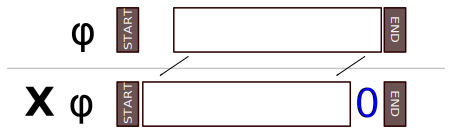
\includegraphics[scale=0.3]{Pattern-X}}~~~
\subfloat[$\mbox{\bf G}\,\varphi$]{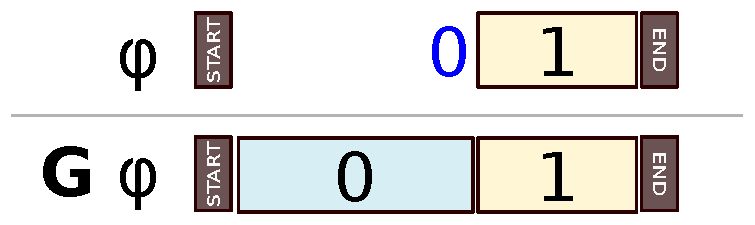
\includegraphics[scale=0.3]{Pattern-G}}~~~
\subfloat[$\varphi\,\mbox{\bf U}\,\psi$]{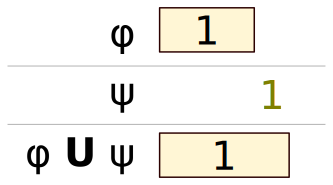
\includegraphics[scale=0.3]{Pattern-U}}
\caption{Une représentation graphique du calcul des trois opérateurs temporels sur bitmaps}
\label{fig:patterns}
\end{figure}

\begin{algorithm}
\caption{Calcul de $\X a$}
\label{alg:next}
\begin{algorithmic}[1]
\Require Bitmap $a$
%\State // X(10101) $\Rightarrow$ (0101)
\State $out \gets$ removeFirstBit($a$)
\State addMany($out$, 0, 1)
\State \Return $out$
\end{algorithmic}
\end{algorithm}

Pour calculer le vecteur de $\G\psi$, il suffit de trouver la plus petite position $i$ de telle sorte que tous les bits suivants sont 1. Dans $B_{\G\psi} $, tous les bits devant $i$ sont mis à 0, et tous les bits d'après (inclusivement) $i$ sont mis à 1. Ainsi, pour mettre en \oe{}uvre cet opérateur avec des bitmaps, nous avons besoin de faire une recherche dans le bitmap $B_{\psi}$ de l'arrière vers l'avant pour trouver la dernière apparition du bit 0, comme on peut le voir de l'Algorithme \ref{alg:global}.

L'opérateur \textbf{F} (montré dans l'Algorithme \ref{alg:future}) est le double de \textbf{G}; son algorithme correspondant fonctionne de la même manière que pour \textbf{G}, en échangeant 0 et 1.

\begin{algorithm}
\caption{Calcul de $\G a$}
\label{alg:global}
\begin{algorithmic}[1]
\Require Bitmap $a$
\State $p \gets$ last(0, $a$)
\If {$p = -1$}
  \State \Return $a$
\Else
  \State $out \gets \langle~\rangle$
  \State addMany($out$, 0, $p + 1$)
  \State addMany($out$, 1, $|a| - p - 1$)
  \State \Return $out$
\EndIf
\end{algorithmic}
\end{algorithm}

\begin{algorithm}
\caption{Calcul de $\F a$}
\label{alg:future}
\begin{algorithmic}[1]
\Require Bitmap $a$
%\State // F(010100) $\Rightarrow$ (111100)
\State $pos \gets$ last(1, $a$)
\If {$pos = -1$}
  \State \Return $a$
\Else
  \State $out \gets$ empty Bitmap
  \State addMany($out$, 1, $pos + 1$)
  \State addMany($out$, 0, $|a| - pos - 1$)
  \State \Return $out$
\EndIf
\end{algorithmic}
\end{algorithm}

D'après la Définition \eqref{eq:until}, s'il y a un indice $j$ avec qui $\overline{s}^j \models \psi$ et $\overline{s}^i$ pour tout $i < j$, alors $\overline{s} \models \varphi\U\psi$. En termes d'opérations bitmap, nous avons besoin de continuer à vérifier s'il y a du bit mis à 1 dans le bitmap $B_{\varphi}$ devant chaque apparition de bit 1 dans $B_{\psi}$ (montré dans l'Algorithme \ref{alg:until}).

\begin{algorithm}
\caption{Calcul de $a \U b$}
\label{alg:until}
\begin{multicols}{2}
\begin{algorithmic}[1]
\Require Bitmaps $a$ et $b$
\State $out \gets \langle~\rangle$
\State $p, a_0, a_1, b_0, b_1 \gets 0$
\While {$p < |a|$}
  \If {$a_1 \leq p$}
    \State $a_1 \gets$ next(1, $a$, $p$)
  \EndIf

  \If {$b_1 \leq p$}
    \State $b_1 \gets$ next(1, $b$, $p$)
  \EndIf

  \If {$a_1 = -1$ or $b_1 = -1$}
    \BreakWhile
  \EndIf

  \State $nearest1 \gets$ min($a_1$, $b_1$)
  \If {$nearest1 > p$}
    %\State // (00..) U (00..) $\Rightarrow$ (00..)
    \State addMany($out$, 0, $nearest1 - p$)
    \State $p \gets nearest1$
    \Continue
  \EndIf

  \If {$p = b_1$}
    %\State // (??..) U (11..) $\Rightarrow$ (11..)
    \If {$b_0 \leq b_1$}
      \State $b_0 \gets$ next(0, $b$, $b_1$)
      \If {$b_0 = -1$}
        \State $b_0 \gets |a|$
      \EndIf
    \EndIf
    \State addMany($out$, 1, $b_0 - p$)
    \State $p \gets b_0$
    \Continue
  \EndIf

  \If {$a_0 \leq a_1$}
    \State $a_0 \gets$ next(0, $a$, $a_1$)
    \If {$a_0 = -1$}
      \State $a_0 \gets |a|$
    \EndIf
  \EndIf
  \If {$a_0 \geq b_1$}
    %\State // (111?..) U (0001..) $\Rightarrow$ (1111..)
    \State addMany($out$, 1, $b_1 - p + 1$)
    \State $p \gets b_1 + 1$
  \Else
    %\State // (11100..) U (00001..) $\Rightarrow$ (00000..)
    \State addMany($out$, 0, $a_0 - p + 1$)
    \State $p \gets a_0 + 1$
  \EndIf
\EndWhile

\If {$b_1 = -1$}
  %\State // (..??) U (..00) $\Rightarrow$ (..00)
  \State addMany($out$, 0, $|a| - |out|$))
\ElsIf {$a_1 = -1$}
  %\State // (..0000) U (..1010) $\Rightarrow$ (..1010)
  \State copyTo($out$, $b$, $p$, $|a| - p$)
\EndIf

\State \Return $out$
\end{algorithmic}
  \end{multicols}
\end{algorithm}

L'opération $\psi \textbf{ W } \varphi$ (la Définition \eqref{eq:wuntil}) est tout à fait semblable à $\psi \textbf{ U } \varphi$, sauf que comme l'implique l'équation \eqref{eq:uw} \citep{huth2004}, l'opération de la première comprend également l'opération $\textbf{G}\psi$. L'Algorithme \ref{alg:wuntil} explique son opération.

\begin{equation} \label{eq:uw}
\psi \textbf{W} \varphi \equiv \psi \textbf{U} \varphi \vee \textbf{G}\psi
\end{equation}

\begin{algorithm}
\caption{Calcul de $a \W b$}
\label{alg:wuntil}
\begin{multicols}{2}
\begin{algorithmic}[1]
\Require Bitmaps $a$ et $b$
\State $out \gets \langle~\rangle$
\State $p, a_0, a_1, b_0, b_1 \gets 0$
\While {p < |a|}
  \If {$a_1 \leq p$}
    \State $a_1 \gets$ next(1, $a$, $p$)
  \EndIf
  \If {$b_1 \leq p$}
    \State $b_1 \gets$ next(1, $b$, $p$)
  \EndIf
  \If {$a_1 = -1$ or $b_1 = -1$}
    \BreakWhile
  \EndIf

  \State $nearest1 \gets$ min($a_1$, $b_1$)
  \If {$nearest1 > p$}
    \State addMany($out$, 0, $nearest1 - p$)
    \State $p \gets nearest1$
    \Continue
  \EndIf

  \If {$p = b_1$}
    \If {$b_0 \leq b_1$}
      \State $b_0 \gets$ next(0, $b$, $b_1$)
      \If {$b_0 = -1$}
        \State $b_0 \gets |a|$
      \EndIf
    \EndIf
    \State addMany($out$, 1, $b_0 - p$)
    \State $p \gets b_0$
    \Continue
  \EndIf

  \If {$a_0 \leq a_1$}
    \State  $a_0 \gets$ next(0, $a$, $a_1$)
    \If {$a_0 = -1$}
      \State $a_0 \gets |a|$
    \EndIf
  \EndIf

  \If {$a_0 \geq b_1$}
    \State addMany($out$, 1, $b_1 - p + 1$)
    \State $p \gets b_1 + 1$
  \Else
    \State addMany($out$, 0, $a_0 - p + 1$)
    \State $p \gets a_0 + 1$
  \EndIf
\EndWhile

\If {$b_1 = -1$}
  \If {$a_1 = -1$}
    \State addMany($out$, 0, $|a| - |out|$)
  \Else
    \State $last0 \gets$ last(0, $a$)
    \If {$last0 = -1$ or $last0 < p$}
      \State addMany($out$, 1, $|a| - |out|$)
    \Else
      \State addMany($out$, 0, $last0 - p + 1$)
      \State addMany($out$, 1, $|a| - |out|$)
    \EndIf
  \EndIf
\ElsIf {$a_1 = -1$}
  \State copyTo($out$, $b$, $|b| - b_1 - 1$, $|b| - b_1$)
\EndIf

\State \Return $out$
\end{algorithmic}
\end{multicols}
\end{algorithm}

Comme le double de l'opérateur \textbf{U}, l'opérateur \textbf{R} défini dans \eqref{eq:release} a besoin de faire une union de deux parties pour la formule $\psi \textbf{ R } \varphi$: la première partie vise à détecter si existent $i, j (0 \leq i < j) $ qui rendent la séquence $\pi^i, \pi^{i + 1}, ... \pi^j $ satisfaite à $\varphi$ lorsque $\pi^j$ satisfait $\psi$; et la seconde est tout simplement $G\varphi$. L'Algorithme \ref{alg:release} décrit cette procédure.

\begin{algorithm}
\caption{Calcul de $a \R b$}
\label{alg:release}
\begin{multicols}{2}
\begin{algorithmic}[1]
\Require Bitmaps $a$ et $b$
\State $out \gets \langle~\rangle$
\State $p, a_0, a_1, b_0, b_1 \gets 0$
\While {$p < |a|$}
  \If {$b_1 \leq p$}
    \State $b_1 \gets$ next(1, $b$, $p$)
  \EndIf
  \If {$b_1 = -1$}
    \BreakWhile
  \EndIf

  \If {$b_1 > p$}
    \State addMany($out$, 0, $b_1 - p$)
    \State $p \gets b_1$
    \Continue
  \EndIf

  \If {$a_1 \leq p$}
    \State $a_1 \gets$ next(1, $a$, $p$)
  \EndIf
  \If {$a_1 = -1$}
    \BreakWhile
  \EndIf

  \If {$b_0 \leq b_1$}
    \State $b_0 \gets$ next(0, $b$, $b_1$)
    \If {$b_0 = -1$}
      \State $b_0 \gets |a|$
    \EndIf
  \EndIf
  \If {$a_1 \geq b_0$}
    \State addMany($out$, 0, $b_0 - p + 1$)
    \State $p \gets b_0 + 1$
    \Continue
  \EndIf

  \If {$a_0 \leq a_1$}
    \State $a_0 \gets$ next(0, $b$, $a_1$)
    \If {$a_0 = -1$}
      \State $a_0 \gets |a|$
    \EndIf
  \EndIf
  \State $nearest0 \gets$ min($a_0$, $b_0$)
  \State addMany($out$, 1, $nearest0 - p$)
  \State $p \gets nearest0$
\EndWhile

\If {$a_1 = -1$ and $b_1 \neq -1$}
  \State $last0 \gets$ last(0, $b$)
  \If {$last0 = -1$ and $last0 < p$}
    \State addMany($out$, 1, $|a| - |out|$)
  \Else
    \State addMany($out$, 0, $last0 - p + 1$)
    \State addMany($out$, 1, $|a| - |out$)
  \EndIf
\Else
  \State addMany($out$, 0, $|a| - |out|$)
\EndIf

\State \Return $out$
\end{algorithmic}
\end{multicols}
\end{algorithm}

\subsection{Discussion}

Un point intéressant des derniers trois algorithmes est que les bitmaps $a$ et $b$ ne sont pas toujours traversés de façon linéaire. Au contraire, des blocs entiers de chaque bitmap peuvent être contournés pour atteindre directement le prochain bit de 0 ou 1, selon le cas. Il faut remarquer que ceci est possible uniquement si la trace est complètement connue à l'avance avant de commencer à évaluer une formule (et de plus, la trace est traversée vers l'arrière). Par conséquent, la solution proposée est un exemple d'un moniteur en mode hors ligne qui n'est pas simplement un moniteur en ligne qui est fourni des événements d'une trace pré-enregistrée un par un: il exploite la possibilité de \emph{accès aléatoire} à des parties de la trace qui est seulement possible dans un réglage hors ligne.

Cet exemple montre l'un des avantages de notre technique proposée en termes de complexité. En effet, la lecture du journal d'origine pour la création des bitmaps fragmentés peut être faite en temps linéaire (et en une seule passe pour tous les symboles propositionnels à la fois). Cependant, une fois que ces bitmaps initiaux sont calculés, un grand nombre des opérations nécessaires ne requièrent plus un traitement linéaire de la trace. Par exemple, l'évaluation $\X\varphi$ nécessite un simple décalage de bits, qui peut être fait dans une seule opération de CPU pour 64 bits à la fois, et potentiellement beaucoup plus si la compression est appliquée.\footnote{Le décalage à gauche de bits d'un bloc compressé est le bloc lui-même, aussi longtemps que le premier bit du prochain bloc à droite a la même valeur.} De la même façon, la recherche du prochain bit de 0 ou 1 requiert rarement la recherche linéaire, car l'utilisation de la compression permet de contourner des mots pleins avec une opération. Le calcul du bitmap pour un opérateur \textbf{F} ou \textbf{G} exige une seule telle recherche pour toute la trace.

Un autre point intéressant est le fait que les opérateurs \textbf{F} et \textbf{G} sont monotones. Comme on peut le voir dans la Figure \ref{fig:patterns}, le bitmap résultant est sous forme de $0^*1^*$ (ou l'inverse). Ainsi, un bitmap très simple se propage vers d'autres algorithmes; il peut être fortement compressé, et rend toute recherche du prochaine 0 ou 1 trivial. Bien que les bitmaps résultant des applications de \textbf{U}, de \textbf{W} et de \textbf{R} ne produisent pas de vecteurs tellement simples, ils ont toujours une structure relativement régulière qui est aussi souple pour la compression raisonnable.

%% }}} --- Subsection

%% }}} --- Section

%% ------------------
%% Section: expériences
%% ------------------
\section{Implémentation et expériences}\label{sec:bm:experiments} %% {{{

Alors que la complexité du pire cas de chaque algorithme présenté dans la section précédente est encore $O(n)$ (où $n$ est la taille du bitmap d'entrée), nous soupçonnons que la performance pratique devrait être beaucoup mieux. Par conséquent, dans cette section, nous décrivons des expériences en vue d'atteindre les objectifs suivants:

\begin{enumerate}
\item Tester la performance des algorithmes LTL fondamentaux;
\item Tester la performance de l'application récursive de ces algorithmes sur des formules LTL complexes;
\item Évaluer la performance et l'espace économique occasionnés grâces à l'utilisation de la compression.
\end{enumerate}

\subsection{Préparation des expériences} %% {{{

Comme un moyen d'éviter les coûts d'entrées ou de sorties de disques à l'exécution, nous chargeons tous les fichiers pertinents dans la mémoire avant les calculs. Ainsi, bien que l'utilisation de bitmaps peut considérablement réduire l'exigence de mémoire, nous avons préparé un poste de travail qui a un processeur d'Intel Xeon E5-2630 v3 et 48 Go de mémoire.

Tous les codes sont mis en \oe{}vre en Java qui prend en soi la responsabilité de la gestion de la mémoire et de la collecte des ordures. En ce qui concerne le délai causé par la collecte des ordures (GC) et surtout Full-GC, nous avons manuellement effectué \textit{System.gc()} avant et après chaque calcul de formules pour fournir un environnement d'exécution qui était aussi ``propre'' que possible.

Le Tableau \ref{table:bmlibs} montre les librairies utilisées pour différents types de bitmap. Afin de mettre en \oe{}uvre toutes les opérations LTL, nous avons modifié les codes des librairies pour ajouter les fonctions nécessaires énumérées dans le Tableau \ref{tbl:bm:bmhelpers} et optimiser les fonctions de sorte que les complexités en temps des opérateurs deviennent $O(m)$ où $m$ est le nombre de séquences de bits consécutifs de 0 ou de 1.

\begin{table}
\centering
\begin{tabular}{|c|l|}
\hline
Librairie bitmap & Source \\
\hline
Non compressée & \texttt{java.util.BitSet} à partir de SDK Java  \\
\hline
\multirow{2}{*}{WAH} & Originale:\ \ \url{https://github.com/metamx/extendedset} \\
& Modifiée: \url{https://github.com/phoenixxie/extendedset} \\
\hline
\multirow{2}{*}{Concise} & Originale:\ \ \url{https://github.com/metamx/extendedset} \\
& Modifiée: \url{https://github.com/phoenixxie/extendedset} \\
\hline
\multirow{2}{*}{EWAH} & Originale:\ \ \url{https://github.com/lemire/javaewah} \\
& Modifiée: \url{https://github.com/phoenixxie/javaewah} \\
\hline
Roaring & \url{https://github.com/lemire/RoaringBitmap} \\
\hline
\end{tabular}
\caption{Librairies bitmap}
\label{table:bmlibs}
\end{table}

En raison du manque de soutien de l'accès aléatoire pour les algorithmes de modèles RLE de compression bitmap, nous ne pouvons pas énumérer les bits de la même manière qu'un bitmap non compressé. Par conséquent, nous avons conçu une structure de données \emph{itérateur} pour stocker non seulement l'indice absolu du bit actuel dans le correspondant bitmap non compressé, mais aussi l'indice relatif dans le bitmap compressé. Prenant l'exemple de la fonction \textbf{next(1, x)}, si l'indice relatif actuel est dans un mot de séquence de 0, la recherche dans ce mot est inutile, et nous passons simplement au mot suivant; si l'indice est dans un mot de séquence de 1, on retourne l'index actuel; cependant, si l'indice est dans un mot littéral, nous devons chercher le bit 1 dans le mot de $ulen$ bits.

Pour les expériences, nous avons développé un générateur de données aléatoires. Chaque fois qu'il génère $5 \times 10^7$ tuples, et chaque tuple contient trois nombres aléatoires ($a, b, c$) liés à trois inégalités simples: $a > 0$, $b > 0$ et $c \leq 0$, qui seront étiquetées comme $s_0$, $s_1$ et $s_2$, respectivement. Selon \eqref{eq:ap}, les valeurs vrai/faux de ces trois déclarations sont composées des propositions atomiques. Quand un tuple a été passé aux trois déclarations, nous avons obtenu trois valeurs booléennes dont chacune a ensuite été transformée en bit de 1 ou de 0 dans le bitmap correspondant à l'un des trois états. Lorsque tous les tuples ont été traités, nous avions trois bitmaps ayant 50 millions de bits chacun.

\subsection{Opérateurs LTL fondamentaux} %% {{{

Une première expérience est formée de l'évaluation de la performance, en termes de temps de calcul, pour évaluer un vecteur de bits sur chaque opérateur propositionnel et temporel.

Dans la première expérience, nous avons effectué 100 passes d'un benchmark sur les opérateurs fondamentaux avec des bitmaps non compressés. Dans chaque passe, les données d'expérience ont été régénérées et transmises aux déclarations relationnelles à partir desquelles les bitmaps ont été créés. Puis les formules ont été exécutées avec les bitmaps. Dans la dernière étape, nous avons calculé le temps moyen d'exécution d'une passe pour chaque opérateur LTL, et le nombre de bits traités par seconde.

Le Tableau \ref{tbl:bm:basicops} montre que les opérateurs logiques propositionnels étaient plus rapides que la plupart des opérateurs logiques temporels. Parmi les opérateurs logiques temporels, les opérateurs binaires sont plus lents que celles unaire parce que les premiers requièrent plus d'opérations que les seconds, particulièrement dans la situation où plusieurs séquences de 0s et de 1s sont mélangées dans le bitmap. Les duals opérateurs \textbf{G} et \textbf{F} ont des algorithmes similaires, mais \textbf{F} a pris étonnamment trois fois plus longtemps que \textbf {G}. Ceci peut être expliqué par le fait que pour un bitmap d'entrée assez randomisé, \textbf{F} ajoute plus de bits de 1s que de 0s à son bitmap de sortie, tandis que \textbf{G} ajoute plus de bits de 0s que de 1s. Bien que l'implémentation de \texttt{BitSet} en Java puisse mettre un bit à 1 et à 0\footnote{\url{https://docs.oracle.com/javase/8/docs/api/java/util/BitSet.html}}, elle ne fait actuellement rien quand elle est demandée de mettre à 0 un nouveau bit dont l'indice est au-delà de sa taille, c'est-à-dire l'ajout d'un bit 0. Il en résulte un traitement asymétrique de bits de 0s et de 1s dans le bitmap.

\begin{table}
\centering
\small
\begin{tabular}{|c|c|c|c|c|}
\hline
Formule & Temps\ Min. & Temps\ Max. & Temps\ Moyen & Débit \\
& (ms) & (ms) & (ms) & (b/s) \\
\hline
$\neg s_0$ & 0 & 15 & 6.18 & $8.09 \times 10^{9}$ \\
\hline
$s_0 \wedge s_1$ & 0 & 16 & 5.86 & $8.53 \times 10^{9}$ \\
\hline
$s_0 \vee s_1$ & 0 & 16 & 5.8 & $8.62 \times 10^{9}$ \\
\hline
$s_0 \rightarrow s_1$ & 0 & 16 & 4.66 & $1.07 \times 10^{10}$ \\
\hline
$\X s_0$ & 0 & 16 & 8.93 & $5.60 \times 10^{9}$ \\
\hline
$\G s_0$ & 46 & 63 & 51.3 & $9.75 \times 10^8$ \\
\hline
$\F s_0$ & 140 & 174 & 150.55 & $3.32 \times 10^8$ \\
\hline
$s_0 \U s_1$ & 1562 & 2017 & 1747.05 & $5.72 \times 10^7$ \\
\hline
$s_0 \W s_1$ & 1531 & 1957 & 1685.71 & $5.93 \times 10^7$ \\
\hline
$s_0 \R s_1$ & 1735 & 2188 & 1961.37 & $5.10 \times 10^7$ \\
\hline
\end{tabular}
\vskip 8pt
\caption{Temps d'exécution d'évaluation de chaque opérateur LTL sur un vecteur de bits, sans l'utilisation de librairie de compression.}
\label{tbl:bm:basicops}
\end{table}

%% }}} --- Subsection

\subsection{Formules complexes} %% {{{

Les résultats de cette première expérience suggèrent que les opérateurs logiques propositionnels, les opérateurs logiques temporels unaires et les opérateurs logiques temporels binaires ont des magnitudes différentes de vitesse de traitement; par conséquent, nous pouvons diviser les opérateurs en trois groupes.

Au début de cette deuxième expérience, nous avons composé diverses combinaisons d'opérateurs en 14 formules LTL avec l'aide de l'outil \emph {randltl} de la librairie \textit{Spot}\footnote{\url{https://spot.lrde.epita.fr/index.html}}; les formules sont présentées dans le Tableau \ref{tbl:bm:complex-formulas}. Ensuite, nous avons également effectué un benchmark de 50 passes sur ces formules avec des bitmaps non compressés. Dans chaque cycle les données ont été régénérées et ré-exécutées avec les 14 formules. Nous avons mesuré le temps d'exécution de chaque cycle et calculé le coût du temps moyen et la vitesse de traitement comme avant.

\begin{table}[h]
\begin{footnotesize}

\begin{equation}\tag{F1}
\G ((s_2 \mathrel{\rightarrow} \F (\mathop{\neg}(s_1 \U  s_2) \W  (s_2 \mathrel{\vee} \G s_1))) \W  (\mathop{\neg}\F (s_0 \R  \X s_2) \W  ((s_0 \mathrel{\wedge} s_2 \mathrel{\wedge} \F s_2) \U  s_0)))
\end{equation}
%
\squeeze
%
\begin{equation}\tag{F2}
\F (\mathop{\neg}(s_2 \mathrel{\rightarrow} \X (s_0 \U  s_1)) \U  (\mathop{\neg}(s_0 \mathrel{\vee} \F \X (s_0 \U  (\X (\F s_1 \W  s_1) \R  s_1))) 
\U  (s_0 \R  \G s_2)))
\end{equation}
%
\squeeze
%
\begin{equation}\tag{F3}
\X \F ((s_1 \mathrel{\vee} s_2 \mathrel{\vee} (\G (s_0 \mathrel{\vee} s_1 \mathrel{\vee} \mathop{\neg}s_1) \mathrel{\wedge} \X \mathop{\neg}s_0)) \mathrel{\rightarrow} \\
((\mathop{\neg}s_0 \mathrel{\rightarrow} (s_0 \mathrel{\wedge} \mathop{\neg}s_1)) \mathrel{\wedge} \G s_0))
\end{equation}
%
\squeeze
%
\begin{equation}\tag{F4}
\X (\mathop{\neg}\G (s_0 \mathrel{\rightarrow} s_2) \mathrel{\rightarrow} \F (s_1 \mathrel{\wedge} ((\F (s_0 \mathrel{\wedge} s_2) \mathrel{\rightarrow} s_1) \mathrel{\rightarrow} \X \mathop{\neg}s_2) \mathrel{\wedge} \G (s_2 \mathrel{\rightarrow} (s_2 \mathrel{\wedge} \F s_1))))
\end{equation}
%
\squeezemore
%
\begin{multline}\tag{F5}
\mathop{\neg}((s_0 \U  (\mathop{\neg}(\mathop{\neg}s_0 \mathrel{\wedge} s_2) \mathrel{\vee} (\mathop{\neg}s_0 \W  (s_2 \mathrel{\rightarrow} s_0)))) \\
\W  \mathop{\neg}s_0) \mathrel{\vee}
(s_1 \R  ((s_1 \mathrel{\vee} (s_0 \W  s_2)) \W  (\mathop{\neg}s_0 \W  s_2)))
\end{multline}
%
\squeeze
%
\begin{equation}\tag{F6}
(s_1 \W  ((s_2 \mathrel{\rightarrow} (\mathop{\neg}s_2 \R  \mathop{\neg}(\mathop{\neg}s_1 \W  s_0))) \W  (\mathop{\neg}s_1 \mathrel{\vee} \mathop{\neg}((\mathop{\neg}s_2 \mathrel{\rightarrow} s_1) \mathrel{\rightarrow} \mathop{\neg}s_0)))) \W  (s_0 \R  \mathop{\neg}s_2)
\end{equation}
%
\squeezemore
%
\begin{multline}\tag{F7}
\X (((\F s_2 \R  s_0) \U  \F s_0) \R  \G ((s_2 \W  s_1) \W  \\
(((\G s_2 \U  s_1) \R  \X s_0) \R  (s_2 \W  ((s_2 \R  \X s_2) \W  s_1)))))
\end{multline}
%
\squeezemore
%
\begin{equation}\tag{F8}
(\G (s_0 \R  \F s_1) \U  \F s_2) \W  \G ((s_1 \U  s_2) \R  ((\G \X s_0 \U  (s_2 \W  s_0)) \W  \F ((\G s_1 \U  s_2) \R  s_2)))
\end{equation}
%
\squeeze
%
\begin{equation}\tag{F9}
\G \F (\G \F s_0 \mathrel{\wedge} \F \X \G s_1 \mathrel{\wedge} \G \F \X \X \X \G \X \F \G s_2)
\end{equation}
%
\squeeze
%
\begin{equation}\tag{F10}
\F \G \F \X (\X s_2 \mathrel{\wedge} \X \G \X \X \G \F (\G \X \F s_1 \mathrel{\wedge} \X \G s_0))
\end{equation}
%
\squeeze
%
\begin{equation}\tag{F11}
\mathop{\neg}(((s_0 \mathrel{\vee} s_2) \mathrel{\rightarrow} (\mathop{\neg}(s_2 \mathrel{\wedge} (\mathop{\neg}s_2 \mathrel{\rightarrow} \mathop{\neg}(s_0 \mathrel{\wedge} (s_0 \mathrel{\vee} \mathop{\neg}s_1)))) \mathrel{\vee} (s_0 \mathrel{\wedge} \mathop{\neg}s_0))) \mathrel{\vee} (\mathop{\neg}s_0 \mathrel{\wedge} (s_0 \mathrel{\vee} s_2)))
\end{equation}
%
\squeezemore
%
\begin{multline}\tag{F12}
(s_1 \mathrel{\wedge} \mathop{\neg}s_2 \mathrel{\wedge} (s_2 \mathrel{\rightarrow} s_0)) \mathrel{\vee} \mathop{\neg}((s_0 \mathrel{\wedge} \mathop{\neg}s_0) \mathrel{\rightarrow} s_1) \mathrel{\vee} \\
((s_2 \mathrel{\vee} (s_1 \mathrel{\rightarrow} s_0)) \mathrel{\wedge} ((s_0 \mathrel{\wedge} \mathop{\neg}s_2 \mathrel{\wedge} (s_1 \mathrel{\rightarrow} s_0)) \mathrel{\rightarrow} s_0))
\end{multline}
%
\squeezemore
%
\begin{multline}\tag{F13}
(((s_0 \W  s_2) \W  s_0) \U  ((s_1 \U  (((s_1 \W  s_2) \W  (s_1 \R  (s_1 \R  s_0))) \W  s_2)) \W  s_2)) \W  \\
((s_0 \R  s_1) \R  (((s_2 \U  s_1) \U  s_1) \R  ((s_0 \W  s_2) \W  s_1)))
\end{multline}
%
\squeezemore
%
\begin{multline}\tag{F14}
((((s_1 \U  s_2) \U  (s_2 \U  s_1)) \U  s_1) \R  (s_1 \R  s_2)) \U  (((s_2 \W  ((s_0 \W  \\
((s_2 \R  s_0) \R  s_1)) \U  s_1)) \W  s_0) \W  (((s_0 \R  s_1) \R  (s_0 \W  s_1)) \U  s_0))
\end{multline}

\end{footnotesize}
\vskip 8pt
\caption{Les formules LTL complexes évaluées expérimentalement}
\label{tbl:bm:complex-formulas}
\end{table}

Comme il est indiqué dans le Tableau \ref{tbl:bm:complex}, trois groupes d'opérateurs ont différentes échelles de vitesse de traitement. Les combinaisons ayant les opérateurs logiques temporels et binaires ont toujours pris plus de temps que d'autres, et les formules F13 et F14 sont les plus lentes. Ce résultat montre également que notre solution peut manipuler un assez grand nombre de bits (événements de la trace) par seconde, allant de millions à des milliards.

\begin{table}[h]
\centering
\small
\begin{tabular}{|c|c|c|c|c|c|c|c|}
\hline
Formule & Opérateurs & Opérateurs & Opérateurs & Temps & Temps & Temps & Bits/second \\
No. & Logiques & Temporels & Temporels. & Min.  & Max. & Avg. & Approx. \\
 & Props. & Unaires & Binaires & (ms) & (ms) & (ms) &  \\
\hline
F1 & 6 & 6 & 6 & 10454 & 14205 & 11483.02 & $1.31 \times 10^7$ \\
\hline
F2 & 4 & 7 & 7 & 7728 & 10673 & 8937.59 & $1.68 \times 10^7$  \\
\hline
F3 & 13 & 5 & 0 & 281 & 422 & 326.63 & $4.59 \times 10^8$  \\
\hline
F4 & 11 & 7 & 0 & 422 & 704 & 560.58 & $2.68 \times 10^8$  \\
\hline
F5 & 11 & 0 & 7 & 8532 & 10496 & 9374.5 & $1.60 \times 10^7$  \\
\hline
F6 & 12 & 0 & 6 & 7280 & 9357 & 7934.6 & $1.89 \times 10^7$  \\
\hline
F7 & 0 & 7 & 11 & 12330 & 15004 & 13413.91 & $1.18 \times 10^7$  \\
\hline
F8 & 0 & 8 & 10 & 9442 & 11833 & 10428.37 & $1.44 \times 10^7$  \\
\hline
F9 & 2 & 16 & 0 & 431 & 1155 & 682.68 & $2.20 \times 10^8$  \\
\hline
F10 & 2 & 16 & 0 & 375 & 857 & 472.76 & $3.17 \times 10^8$  \\
\hline
F11 & 18 & 0 & 0 & 31 & 56 & 45.18 & $3.32 \times 10^9$  \\
\hline
F12 & 18 & 0 & 0 & 46 & 68 & 51.58 & $2.91 \times 10^9$  \\
\hline
F13 & 0 & 0 & 18 & 22768 & 27308 & 24825.21 & $6.04 \times 10^6$  \\
\hline
F14 & 0 & 0 & 18 & 22800 & 27481 & 24877.67 & $6.03 \times 10^6$  \\
\hline
\end{tabular}
\vskip 8pt
\caption{Temps d'exécution de l'évaluation des formules LTL du Tableau \ref{tbl:bm:complex-formulas}, sans l'utilisation de librairie de compression.}
\label{tbl:bm:complex}
\end{table}

%% }}} --- Subsection

\subsection{Utilisation de compression bitmap} %% {{{

Selon les algorithmes de modèles RLE, le taux de compression dépend principalement de la longueur de bits consécutifs de 0s ou de 1s. De ce fait, dans cette expérience, nous avons modifié le générateur pour lui permettre de répéter le même tuple un certain nombre de fois: 1, 32 et 64. Ce nouveau mécanisme est en mesure d'assurer l'existence de séquences continues d'une longueur minimum ($slen$) dans les bitmaps générés. Intuitivement, lorsque la valeur de $slen$ augmente, le nombre de séquences diminue; par conséquent, les algorithmes de modèles RLE devraient avoir de meilleures performances qu'un bitmap non compressé.

\begin{figure}[h]
\begin{center}
\centering
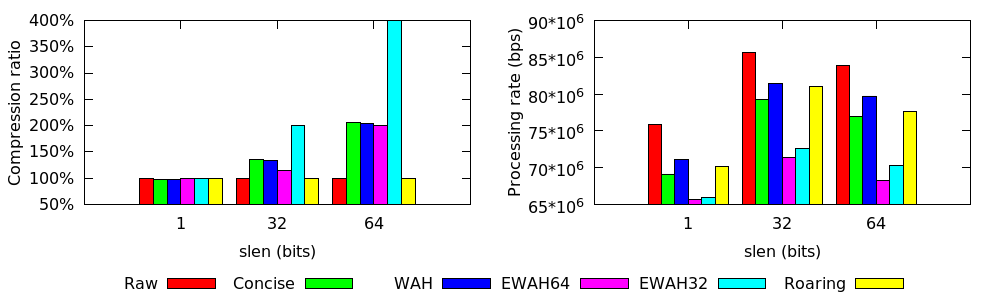
\includegraphics[width=\linewidth]{states.png}
\caption{Génération de bitmaps avec les algorithmes de compression}
\label{img:states}
\end{center}
\end{figure}

Dans la première partie de l'expérience, nous avons généré les bitmaps avec les algorithmes différents et les valeurs différentes de $slen$, puis calculé les taux de compression. Le résultat dans la Figure \ref{img:states} confirme l'hypothèse selon laquelle quand $slen < wlen$ (où $wlen$ est la longueur d'un mot), le bitmap ne peut pas être bien compressé par un algorithme de modèle RLE, et dans ce cas, l'algorithme EWAH se comporte un peu mieux que les autres en raison de son coût structurel plus petit. Lorsque $slen$ augmente à 32 et à 64, c.-à-d. $slen \geq wlen$, les algorithmes RLE commencent à bien fonctionner et le taux de compression lors de $slen = 64$ est évidemment meilleure que celui lors de $slen = 32$. De la Figure \ref{img:states}, nous pouvons également voir que quand $slen$ est égal à 1, à 32 et à 64, EWAHs sont plus lents que WAH, Concise et Roaring.

Dans la deuxième partie de l'expérience, nous avons mesuré les performances des bitmaps compressés lors de l'application des algorithmes pour tous les opérateurs fondamentaux et tous les formules LTL dans les expériences précédentes. Les résultats détaillés couvrant tous les opérateurs et les formules peuvent être trouvés dans l'Annexe \ref{appendixa}.

À cette fin, nous avons choisi les formules F1 et F14 de l'expérience précédente, car F1 contient tous les opérateurs et les conjonctions de LTL et F14 est la plus lente de toutes les formules dans l'expérience précédente. Nous avons à nouveau effectué le benchmark 100 fois; dans chaque cycle, la formule a été évalué par un groupe de bitmaps d'entrée de la dernière étape et nous avons enregistré le coût de temps de chaque algorithme bitmap et de chaque longueur de bits consécutifs.

\begin{figure}[h]
\begin{center}
\centering
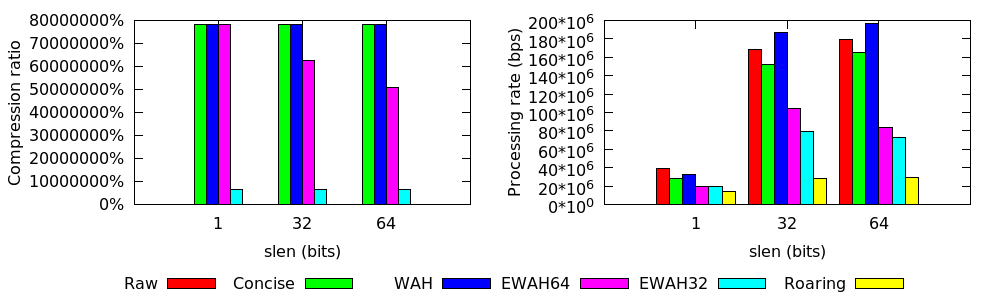
\includegraphics[width=\linewidth]{p11.png}
\caption{Comparaison du taux de compression et de la vitesse de traitement de la formule F1, avec diverses librairies de compression bitmap et différentes valeurs de $slen$}
\label{img:f1}
\end{center}
\end{figure}

\begin{figure}[h]
\begin{center}
\centering
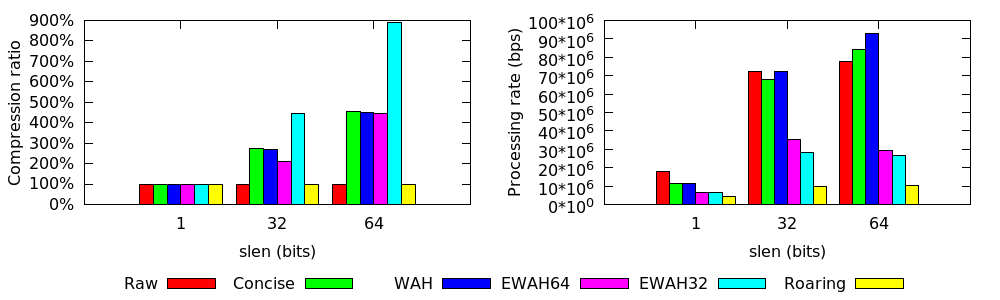
\includegraphics[width=\linewidth]{p24.png}
\caption{Comparaison du taux de compression et de la vitesse de traitement de la formule F14, avec diverses librairies de compression bitmap et différentes valeurs de $slen$}
\label{img:f14}
\end{center}
\end{figure}

Selon les Figures \ref{img:f1} et \ref{img:f14}, la performance des algorithmes de modèles RLE, WAH, EWAH et Concise est évidemment liée à la valeur de $slen$. La Figure \ref{img:f1} suggère également que la présence des opérateurs \textbf{G} et \textbf{F} peut grandement augmenter la longueur de bits consécutifs de même valeur, qui à leur tour peuvent être bien compressés par des algorithmes de modèles RLE. Dans un tel cas, plusieurs algorithmes ont de meilleures performances que le bitmap non compressé lors de l'augmentation de $slen$.

%% }}} --- Subsection

%% }}} --- Section

%% ------------------
%% Section: related work
%% ------------------
\section{Travaux connexes}\label{sec:bm:related} %% {{{

La perspective de l'utilisation de propriétés physiques de matériel pour améliorer les performances de la vérification de l'exécution a déjà été étudiée dans le passé récent. Par exemple, Pellizzoni \etal\@ \citep{pellizzoni2008hardware} ont utilisé du dédié matériel commercial-off-the-shelf (COTS) \citep{emerson1990temporal} pour faciliter le monitoring de l'exécution de systèmes embarqués critiques dont les propriétés ont été exprimées en logique temporelle linéaire en temps passé (ptLTL).

Comme le nombre de c\oe{}urs (GPU ou CPU multi-c\oe{}urs) dans le matériel de base ne cesse de croître, la recherche de l'exploitation des processeurs disponibles ou des c\oe{}ur disponibles pour paralléliser les tâches et les calculs apporte un défi et aussi une occasion d'amélioration de l'architecture de la vérification de l'exécution. Par exemple, Ha \etal\@ \citep{ha2009concurrent} ont présenté une conception de tamponnage de \emph{Cache-friendly Asymmetric Buffering (CAB)} pour améliorer les communications entre l'application et le moniteur d'exécution en utilisant le cache partagé de l'architecture multi-c\oe{}urs; Berkovich \etal\@ \citep{DBLP:journals/fmsd/BerkovichBF15} a proposé une solution à base de GPU qui utilise efficacement les c\oe{}urs disponibles du GPU, de sorte que le moniteur conçu et implémenté avec leur méthode peut fonctionner en parallèle avec le programme cible et évaluer des propriétés LTL.

Le travail antérieur de l'un des auteurs \citep{jocasa} introduit un algorithme pour la vérification automatisée de formules de logiques temporelles linéaires sur des traces d'événements, en utilisant un plus en plus populaire cadre de cloud computing appelé MapReduce. L'algorithme peut traiter plusieurs fragments arbitraires de la trace en parallèle, et calculer le résultat final à travers un cycle d'exécution d'instances de MapReduce.
La technique proposée manipule des objets appelés \emph{tuples}, qui sont de la forme $\langle \phi, (n, i)\rangle$, et sont interprétés comme la déclaration ``the process is at iteration $i$, and LTL formula $\phi$ is true for the suffix of the current trace starting at its $n$-th event''. On peut voir que cette déclaration correspond exactement au fait, dans la présente solution, que la $n$-ème position du bitmap généré par l'évaluation de $\phi$ contient la valeur 1.

Outre cette similitude, toutefois, les deux techniques sont radicalement différentes. Puisque la méthode de MapReduce fonctionne sur les tuples un par un, alors que la présente solution manipule les bitmaps entiers, les algorithmes pour chaque opérateur LTL ont peu en commun (en particulier celui de \textbf{U}). Lorsque la méthode de MapReduce obtient sa vitesse du traitement de plusieurs sous-formules sur des machines différentes, notre solution présente est efficace parce que certaines opérations (comme conjonction) peuvent être calculées simultanément pour de nombreux événements adjacents dans un seul cycle de CPU. En plus, un inconvénient de la solution MapReduce est le grand nombre de tuples générées, et l'impossibilité de compression du volume de données.

Comme on peut le voir, il y avait plusieurs tentatives de s'appuyer le parallélisme et les propriétés de matériel pour évaluer les expressions temporelles sur des traces. Cependant, pour autant que l'on le sache, notre travail est le premier à obtenir l'amélioration de performance au niveau de la \emph{structures de données} pour évaluer ces expressions.

%% }}} --- Section

%% ------------------
%% Section: conclusion
%% ------------------
\section{Conclusion et perspectives}\label{sec:bm:conclusion} %% {{{

Nous avons proposé une solution pour l'évaluation hors ligne de formules LTL au moyen de manipulation de bitmaps. Dans un tel contexte, les prédicats propositionnel d'événements individuels d'états d'une trace sont mappés aux bits d'un vecteur (``bitmap'') qui sont ensuite manipulés pour mettre en \oe{}uvre chaque opérateur LTL. En plus du fait que les manipulations de bitmaps sont en soi très efficaces, nos algorithmes profitent du fait que la trace est complètement connue à l'avance, et que l'accès aléatoire à une position quelconque de cette trace permet de contourner de grands blocs d'événements pour accélérer l'évaluation.

Pour cette raison, notre solution est un important exemple d'un algorithme d'évaluation hors ligne qui exploite le fait que cela fonctionne bien en mode hors ligne --- il n'est pas un algorithme en ligne qui lit les événements à partir d'une trace pré-enregistré un par un. En fait, dans certains cas (comme l'opérateur \textbf{U}), la trace est même évaluée à partir de la fin, plutôt que à partir du début. Un approfondi benchmark de performance pour les opérateurs fondamentaux et les formules LTL complexes a prouvé la faisabilité de la solution, et a montré comment les événements d'une trace peuvent être traités à une vitesse allant de millions à des milliards d'événements par seconde.

Pour exploiter davantage le potentiel de bitmap, nous avons présenté des algorithmes de compression bitmap dans notre solution et les avons intégrés dans notre benchmark. Dans les expériences, comme nous l'espérions, notre solution a démontré sa capacité de compresser facilement les creux bitmaps et d'accélérer les opérations LTL quand il y a un certain nombre de bits consécutifs avec la même valeur. Nous avons expliqué, comment de nombreux opérateurs LTL augmentent naturellement la régularité des bitmaps qu'ils traitent.

De toute évidence, cette solution ne convient que à l'évaluation hors ligne. Cependant, les résultats prometteurs obtenus dans notre implémentation conduisent à un grand nombre d'extensions et d'améliorations potentielles basées sur la méthode actuelle. Tout d'abord, l'algorithme peut être réutilisé comme base pour d'autres langages temporels qui se croisent avec LTL, tels que PSL \citep{IntroPSLBook}. D'autre part, cette technique pourrait être étendue pour prendre en considération des paramètres et de la quantification de données. Enfin, on pourrait aussi envisager la parallélisation de l'évaluation de grands segments de bitmaps sur plusieurs machines.
%% }}} --- Section

%% :folding=explicit:wrap=soft:mode=latex:


%% ...
%% Ajoutez autant de commandes include qu'il y a de chapitres à
%% inclure dans votre document
%% ...
%!TEX root = these.tex

\chapter{Conclusion and future work}

Software verification and validation is a critical part in software engineering and project management. People have learned this from lots of lessons in the past ranging from crashed games to fatal disaster. Comparing with traditional techniques of software verification, runtime verification is relatively new. It has root in other techniques and it has its own feature. In recent years, a great amount of work and time has been invested in various aspects of this area. Some researchers focus on the improvement and applications of various variant of LTL, and some others manage to develop more and more generic frameworks.

Although network has already covered much place on earth, many networking mediums have been exploited and various networking protocols have been proposed, there is still some place where cable and wireless radio have not reached, like deserts or underwater, or some environment where both cable and wireless radio are undesirable or even forbidden, for example, in planes, hospitals, mines or petro-chemical plants. Even under these limitations, software verification is as essential as in networking-covered places. Visible light communication (VLC) is an efficient solution in these situations and has many successful solutions, which enlightened us to think of a method of using optical codes for the data communication work. QR code is encoded optical label which is able to store considerable data and to efficiently encode and decode data, which gave us the confidence to apply it in our solution.

In the first part of our research, the goal was to design and implement an one-way QR Code communication channel. In the development, we used the computer programming language Java and the well-known QR Code library ZXing. In early experiment, we tested the characteristics of a QR data stream and found that due to the limitation of the hardwares we used, the data loss rate was impossibly zero and it grew fast as the data size of each frame increased. Therefore on one hand we managed to improve the recognition rate of QR codes by adjusting the options of the ZXing library and the camera. On the other hand we proposed the protocol BufferTannen which is in charge of splitting, marshaling, and to some extend compressing the data to transmit. The final result presented in Section \ref{sec:qr:experiments} proves the feasibility of our solution. This part of our research has been published in the journal IEEE Access in 2016.

Every software system, no matter operation systems of mobile phones, web applications, or cloud computing system, needs to guarantee its smooth running and response in time for the exceptions in order to reduce the loss or avoid the disaster. The requirement of software verification for each system could be similar, as is suggested in Section \ref{sec:rv:frameworks} which introduced several runtime verification frameworks sharing same functionalities. However, the scale of every software systems varies a lot. For example, a smartphone has much lower memory and slower processor than a mainstream workstation, not to mention a cloud computing system like Amazon EC2. When developing a RV system for a smartphone, the usage of memory and processor is always the main concern. In another way, even in a computer system which has huge memory and power processor, there is always a limit to the memory and the processor. Therefore, there are many researches on the improvement of RV systems. Some tried to distribute the computing to a cluster of servers, some managed to optimize the algorithms or find a better solution.

Our second objective was to find a way to improve the speed of LTL formul\ae{}s' calculation. Bitmap is a compact and efficient data structure which has a lot of applications and solutions. A verdict issued by offline runtime verification monitor is two-valued truth value, which can be easily mapped into a bit in a bitmap. We also designed a few algorithms to implement the LTL operators with mapped bitmaps. \cite{lemire2014} suggests that a sparse bitmap can be well compressed, and as we discussed in Section \ref{sec:bm:ltlbitmap}, the output bitmap from the algorithms has longer consecutive 1/0 sequence than the input. Therefore we integrated bitmap compression algorithms into our solution. The experiment results demonstrate the performance and the feasibility of our solution, and prove that the usage of bitmap compression can make our solution faster and more space-efficient with certain algorithms. This part of our research is also written in a paper which is still under review for publication in the proceedings of the International Conference: Runtime Verification 2016 (RV'16) in Madrid, Spain in 2016.

\section*{Future work}

Our QR code communication channel supports only one-way data transfer, resulting that even our program resends the same data frame for several times, we still cannot ensure that the receiver has got all the data. A bidirectional communication seems an answer to this problem, and it can also allow to resend data on demand and thus increase the effective bandwidth.

A bitmap has bits of either 1 or 0, so the $inconclusive$ value of LTL$_3$ cannot be easily implemented. As a result, our solution works only in the offline monitoring mode. To support the online mode is a big but interesting challenge. In addition, making our solution parallelized to be able to run in a computing cloud is also very intriguing.

% \begin{appendices}
% %!TEX root = these.tex

In this appendix, we present the experiment results of the third part of Section \ref{sec:bm:experiments}. To get better formatting, the data format is different than it in Section \ref{sec:bm:experiments}. ``Ratio'' here has not percentage mark because it is compression rate calculated by the division of original data size and compressed size.

\begin{table}[h]
\small
\centering
\makebox[\linewidth]{
\begin{tabular}{|c|c|c|c|c|c|c|c|c|c|c|}
\hline
& $slen$ & \multicolumn{3}{|c|}{1} & \multicolumn{3}{|c|}{32} & \multicolumn{3}{|c|}{64} \\
\hline
Type & & Min & Max & Avg. & Min & Max & Avg. & Min & Max & Avg. \\
\hline
\multirow{2}{*}{Raw} & Ratio & 1.00 & 1.00 & 1.00 & 1.00 & 1.00 & 1.00 & 1.00 & 1.00 & 1.00 \\
\cline{2-11}
& bps & 6.44E+7 & 8.32E+7 & 7.59E+7 & 7.64E+7 & 9.18E+7 & 8.57E+7 & 7.40E+7 & 9.27E+7 & 8.39E+7 \\
\hline
\multirow{2}{*}{Concise} & Ratio & 0.97 & 0.97 & 0.97 & 1.35 & 1.35 & 1.35 & 2.06 & 2.07 & 2.07 \\
\cline{2-11}
& bps & 6.18E+7 & 7.60E+7 & 6.91E+7 & 6.99E+7 & 8.56E+7 & 7.93E+7 & 6.67E+7 & 8.47E+7 & 7.70E+7 \\
\hline
\multirow{2}{*}{WAH} & Ratio & 0.97 & 0.97 & 0.97 & 1.33 & 1.34 & 1.33 & 2.03 & 2.04 & 2.03 \\
\cline{2-11}
& bps & 6.28E+7 & 7.84E+7 & 7.12E+7 & 7.23E+7 & 8.86E+7 & 8.15E+7 & 6.58E+7 & 8.95E+7 & 7.97E+7 \\
\hline
\multirow{2}{*}{EWAH64} & Ratio & 1.00 & 1.00 & 1.00 & 1.14 & 1.14 & 1.14 & 1.99 & 2.01 & 2.00 \\
\cline{2-11}
& bps & 5.66E+7 & 7.29E+7 & 6.56E+7 & 6.24E+7 & 7.62E+7 & 7.14E+7 & 5.99E+7 & 7.58E+7 & 6.83E+7 \\
\hline
\multirow{2}{*}{EWAH32} & Ratio & 1.00 & 1.00 & 1.00 & 2.00 & 2.00 & 2.00 & 3.99 & 4.01 & 4.00 \\
\cline{2-11}
& bps & 5.82E+7 & 7.34E+7 & 6.59E+7 & 6.48E+7 & 7.74E+7 & 7.26E+7 & 6.09E+7 & 7.73E+7 & 7.03E+7 \\
\hline
\multirow{2}{*}{Roaring} & Ratio & 1.00 & 1.00 & 1.00 & 1.00 & 1.00 & 1.00 & 1.00 & 1.00 & 1.00 \\
\cline{2-11}
& bps & 6.11E+7 & 7.78E+7 & 7.01E+7 & 7.04E+7 & 8.72E+7 & 8.10E+7 & 6.78E+7 & 8.88E+7 & 7.76E+7 \\
\hline
\end{tabular}
}
\caption{Bitmap generation with compression algorithms}
\end{table}

\begin{table}[h]
\small
\centering
\makebox[\linewidth]{
\begin{tabular}{|c|c|c|c|c|c|c|c|c|c|c|}
\hline
& $slen$ & \multicolumn{3}{|c|}{1} & \multicolumn{3}{|c|}{32} & \multicolumn{3}{|c|}{64} \\
\hline
Type & & Min & Max & Avg. & Min & Max & Avg. & Min & Max & Avg. \\
\hline
\multirow{2}{*}{Raw} & Ratio & 1.00 & 1.00 & 1.00 & 1.00 & 1.00 & 1.00 & 1.00 & 1.00 & 1.00 \\
\cline{2-11}
& bps & 3.00E+10 & 4.50E+11 & 7.28E+10 & 4.50E+10 & 7.50E+10 & 5.79E+10 & 2.65E+10 & 6.43E+10 & 5.17E+10 \\
\hline
\multirow{2}{*}{Concise} & Ratio & 0.97 & 0.97 & 0.97 & 1.35 & 1.35 & 1.35 & 2.06 & 2.07 & 2.07 \\
\cline{2-11}
& bps & 7.37E+9 & 3.32E+10 & 1.24E+10 & 1.45E+10 & 2.09E+10 & 1.84E+10 & 1.04E+10 & 1.68E+10 & 1.35E+10 \\
\hline
\multirow{2}{*}{WAH} & Ratio & 0.97 & 0.97 & 0.97 & 1.33 & 1.34 & 1.33 & 2.03 & 2.04 & 2.03 \\
\cline{2-11}
& bps & 9.48E+9 & 4.65E+11 & 1.80E+10 & 3.75E+10 & 4.82E+10 & 4.34E+10 & 3.16E+10 & 4.43E+10 & 3.84E+10 \\
\hline
\multirow{2}{*}{EWAH64} & Ratio & 1.00 & 1.00 & 1.00 & 1.14 & 1.14 & 1.14 & 1.99 & 2.00 & 2.00 \\
\cline{2-11}
& bps & 2.65E+10 & 4.50E+11 & 3.03E+10 & 1.57E+10 & 2.07E+10 & 1.85E+10 & 1.13E+10 & 1.41E+10 & 1.27E+10 \\
\hline
\multirow{2}{*}{EWAH32} & Ratio & 1.00 & 1.00 & 1.00 & 2.00 & 2.00 & 2.00 & 3.99 & 4.01 & 4.00 \\
\cline{2-11}
& bps & 1.41E+10 & 3.00E+10 & 1.67E+10 & 1.12E+10 & 1.25E+10 & 1.19E+10 & 5.63E+9 & 7.03E+9 & 6.45E+9 \\
\hline
\multirow{2}{*}{Roaring} & Ratio & 1.00 & 1.00 & 1.00 & 1.00 & 1.00 & 1.00 & 1.00 & 1.00 & 1.00 \\
\cline{2-11}
& bps & 2.81E+10 & 4.50E+11 & 6.48E+10 & 5.00E+10 & 6.43E+10 & 5.76E+10 & 4.50E+10 & 6.43E+10 & 5.66E+10 \\
\hline
\end{tabular}
}
\caption{Calculation of $\neg s_0$ with compression algorithms}
\end{table}


\begin{table}[h]
\small
\centering
\makebox[\linewidth]{
\begin{tabular}{|c|c|c|c|c|c|c|c|c|c|c|}
\hline
& $slen$ & \multicolumn{3}{|c|}{1} & \multicolumn{3}{|c|}{32} & \multicolumn{3}{|c|}{64} \\
\hline
Type & & Min & Max & Avg. & Min & Max & Avg. & Min & Max & Avg. \\
\hline
\multirow{2}{*}{Raw} & Ratio & 1.00 & 1.00 & 1.00 & 1.00 & 1.00 & 1.00 & 1.00 & 1.00 & 1.00 \\
\cline{2-11}
& bps & 2.81E+10 & 4.50E+11 & 7.68E+10 & 6.43E+10 & 9.00E+10 & 7.48E+10 & 5.00E+10 & 9.00E+10 & 7.20E+10 \\
\hline
\multirow{2}{*}{Concise} & Ratio & 0.97 & 0.97 & 0.97 & 1.79 & 1.80 & 1.80 & 2.74 & 2.77 & 2.76 \\
\cline{2-11}
& bps & 5.96E+9 & 1.50E+10 & 8.93E+9 & 3.84E+9 & 4.77E+9 & 4.23E+9 & 2.72E+9 & 3.35E+9 & 2.98E+9 \\
\hline
\multirow{2}{*}{WAH} & Ratio & 0.97 & 0.97 & 0.97 & 1.77 & 1.78 & 1.78 & 2.70 & 2.72 & 2.71 \\
\cline{2-11}
& bps & 9.29E+9 & 2.90E+10 & 1.34E+10 & 3.92E+9 & 5.92E+9 & 5.54E+9 & 3.88E+9 & 4.61E+9 & 4.34E+9 \\
\hline
\multirow{2}{*}{EWAH64} & Ratio & 1.00 & 1.00 & 1.00 & 1.47 & 1.47 & 1.47 & 2.66 & 2.68 & 2.67 \\
\cline{2-11}
& bps & 1.41E+10 & 3.00E+10 & 1.83E+10 & 4.92E+9 & 6.67E+9 & 6.02E+9 & 3.81E+9 & 4.79E+9 & 4.33E+9 \\
\hline
\multirow{2}{*}{EWAH32} & Ratio & 1.00 & 1.00 & 1.00 & 2.66 & 2.67 & 2.67 & 5.31 & 5.35 & 5.33 \\
\cline{2-11}
& bps & 9.18E+9 & 1.55E+10 & 1.29E+10 & 3.04E+9 & 3.57E+9 & 3.26E+9 & 1.94E+9 & 2.34E+9 & 2.21E+9 \\
\hline
\multirow{2}{*}{Roaring} & Ratio & 1.00 & 1.00 & 1.00 & 1.00 & 1.00 & 1.00 & 1.00 & 1.00 & 1.00 \\
\cline{2-11}
& bps & 1.41E+10 & 3.00E+10 & 2.37E+10 & 2.37E+10 & 2.81E+10 & 2.54E+10 & 2.25E+10 & 2.81E+10 & 2.52E+10 \\
\hline
\end{tabular}
}
\caption{Calculation of $s_0 \wedge s_1$ with compression algorithms}
\end{table}


\begin{table}[h]
\small
\centering
\makebox[\linewidth]{
\begin{tabular}{|c|c|c|c|c|c|c|c|c|c|c|}
\hline
& $slen$ & \multicolumn{3}{|c|}{1} & \multicolumn{3}{|c|}{32} & \multicolumn{3}{|c|}{64} \\
\hline
Type & & Min & Max & Avg. & Min & Max & Avg. & Min & Max & Avg. \\
\hline
\multirow{2}{*}{Raw} & Ratio & 1.00 & 1.00 & 1.00 & 1.00 & 1.00 & 1.00 & 1.00 & 1.00 & 1.00 \\
\cline{2-11}
& bps & 2.81E+10 & 4.50E+11 & 7.76E+10 & 5.00E+10 & 9.00E+10 & 7.13E+10 & 5.00E+10 & 9.00E+10 & 6.63E+10 \\
\hline
\multirow{2}{*}{Concise} & Ratio & 0.97 & 0.97 & 0.97 & 1.79 & 1.80 & 1.80 & 2.74 & 2.77 & 2.76 \\
\cline{2-11}
& bps & 7.74E+9 & 1.50E+10 & 1.25E+10 & 3.93E+9 & 6.42E+9 & 5.04E+9 & 2.59E+9 & 4.84E+9 & 3.52E+9 \\
\hline
\multirow{2}{*}{WAH} & Ratio & 0.97 & 0.97 & 0.97 & 1.77 & 1.78 & 1.78 & 2.70 & 2.72 & 2.71 \\
\cline{2-11}
& bps & 1.26E+10 & 3.10E+10 & 1.87E+10 & 6.14E+9 & 1.05E+10 & 9.07E+9 & 6.92E+9 & 9.22E+9 & 8.25E+9 \\
\hline
\multirow{2}{*}{EWAH64} & Ratio & 1.00 & 1.00 & 1.00 & 1.47 & 1.47 & 1.47 & 2.65 & 2.68 & 2.67 \\
\cline{2-11}
& bps & 1.41E+10 & 3.00E+10 & 2.01E+10 & 5.55E+9 & 7.43E+9 & 6.66E+9 & 4.41E+9 & 5.49E+9 & 4.88E+9 \\
\hline
\multirow{2}{*}{EWAH32} & Ratio & 1.00 & 1.00 & 1.00 & 2.66 & 2.67 & 2.67 & 5.31 & 5.35 & 5.33 \\
\cline{2-11}
& bps & 9.57E+9 & 1.50E+10 & 1.30E+10 & 3.46E+9 & 4.50E+9 & 3.86E+9 & 2.30E+9 & 2.96E+9 & 2.54E+9 \\
\hline
\multirow{2}{*}{Roaring} & Ratio & 1.00 & 1.00 & 1.00 & 1.00 & 1.00 & 1.00 & 1.00 & 1.00 & 1.00 \\
\cline{2-11}
& bps & 2.81E+10 & 4.50E+11 & 3.94E+10 & 3.22E+10 & 3.75E+10 & 3.52E+10 & 3.22E+10 & 3.75E+10 & 3.47E+10 \\
\hline
\end{tabular}
}
\caption{Calculation of $s_0 \vee s_1$ with compression algorithms}
\end{table}


\begin{table}[h]
\small
\centering
\makebox[\linewidth]{
\begin{tabular}{|c|c|c|c|c|c|c|c|c|c|c|}
\hline
& $slen$ & \multicolumn{3}{|c|}{1} & \multicolumn{3}{|c|}{32} & \multicolumn{3}{|c|}{64} \\
\hline
Type & & Min & Max & Avg. & Min & Max & Avg. & Min & Max & Avg. \\
\hline
\multirow{2}{*}{Raw} & Ratio & 1.00 & 1.00 & 1.00 & 1.00 & 1.00 & 1.00 & 1.00 & 1.00 & 1.00 \\
\cline{2-11}
& bps & 2.81E+10 & 4.50E+11 & 9.66E+10 & 5.00E+10 & 1.12E+11 & 7.39E+10 & 2.81E+10 & 9.00E+10 & 5.78E+10 \\
\hline
\multirow{2}{*}{Concise} & Ratio & 0.97 & 0.97 & 0.97 & 1.79 & 1.80 & 1.80 & 2.74 & 2.77 & 2.75 \\
\cline{2-11}
& bps & 7.37E+9 & 2.90E+10 & 1.17E+10 & 6.30E+9 & 8.35E+9 & 7.22E+9 & 4.84E+9 & 6.40E+9 & 5.63E+9 \\
\hline
\multirow{2}{*}{WAH} & Ratio & 0.97 & 0.97 & 0.97 & 1.77 & 1.78 & 1.78 & 2.70 & 2.72 & 2.71 \\
\cline{2-11}
& bps & 9.88E+9 & 1.94E+10 & 1.36E+10 & 6.75E+9 & 9.64E+9 & 8.07E+9 & 6.15E+9 & 7.63E+9 & 6.92E+9 \\
\hline
\multirow{2}{*}{EWAH64} & Ratio & 1.00 & 1.00 & 1.00 & 1.47 & 1.48 & 1.47 & 2.65 & 2.68 & 2.67 \\
\cline{2-11}
& bps & 1.29E+10 & 3.00E+10 & 1.50E+10 & 5.18E+9 & 1.16E+10 & 8.60E+9 & 4.33E+9 & 7.76E+9 & 6.58E+9 \\
\hline
\multirow{2}{*}{EWAH32} & Ratio & 1.00 & 1.00 & 1.00 & 2.66 & 2.68 & 2.67 & 5.30 & 5.36 & 5.33 \\
\cline{2-11}
& bps & 1.41E+10 & 3.00E+10 & 1.87E+10 & 3.26E+9 & 4.41E+9 & 3.76E+9 & 2.45E+9 & 4.17E+9 & 3.50E+9 \\
\hline
\multirow{2}{*}{Roaring} & Ratio & 1.00 & 1.00 & 1.00 & 1.00 & 1.00 & 1.00 & 1.00 & 1.00 & 1.00 \\
\cline{2-11}
& bps & 2.81E+10 & 4.50E+11 & 4.69E+10 & 3.75E+10 & 6.43E+10 & 5.05E+10 & 3.75E+10 & 6.43E+10 & 4.95E+10 \\
\hline
\end{tabular}
}
\caption{Calculation of $s_0 \vee s_1$ with compression algorithms}
\end{table}


\begin{table}[h]
\small
\centering
\makebox[\linewidth]{
\begin{tabular}{|c|c|c|c|c|c|c|c|c|c|c|}
\hline
& $slen$ & \multicolumn{3}{|c|}{1} & \multicolumn{3}{|c|}{32} & \multicolumn{3}{|c|}{64} \\
\hline
Type & & Min & Max & Avg. & Min & Max & Avg. & Min & Max & Avg. \\
\hline
\multirow{2}{*}{Raw} & Ratio & 1.00 & 1.00 & 1.00 & 1.00 & 1.00 & 1.00 & 1.00 & 1.00 & 1.00 \\
\cline{2-11}
& bps & 2.81E+10 & 4.50E+11 & 5.04E+10 & 4.50E+10 & 5.62E+10 & 5.06E+10 & 4.09E+10 & 5.62E+10 & 4.95E+10 \\
\hline
\multirow{2}{*}{Concise} & Ratio & 0.97 & 0.97 & 0.97 & 1.35 & 1.35 & 1.35 & 2.06 & 2.07 & 2.07 \\
\cline{2-11}
& bps & 1.50E+10 & 3.10E+10 & 1.80E+10 & 8.14E+9 & 1.04E+10 & 9.44E+9 & 4.84E+9 & 6.80E+9 & 6.22E+9 \\
\hline
\multirow{2}{*}{WAH} & Ratio & 0.97 & 0.97 & 0.97 & 1.33 & 1.34 & 1.33 & 2.03 & 2.04 & 2.03 \\
\cline{2-11}
& bps & 1.45E+10 & 3.10E+10 & 1.86E+10 & 7.34E+9 & 1.16E+10 & 1.04E+10 & 5.40E+9 & 7.91E+9 & 7.21E+9 \\
\hline
\multirow{2}{*}{EWAH64} & Ratio & 1.00 & 1.00 & 1.00 & 1.07 & 1.07 & 1.07 & 1.33 & 1.34 & 1.33 \\
\cline{2-11}
& bps & 1.41E+10 & 3.00E+10 & 2.23E+10 & 1.01E+10 & 1.41E+10 & 1.28E+10 & 5.11E+9 & 6.82E+9 & 6.09E+9 \\
\hline
\multirow{2}{*}{EWAH32} & Ratio & 1.00 & 1.00 & 1.00 & 1.33 & 1.34 & 1.33 & 1.99 & 2.00 & 2.00 \\
\cline{2-11}
& bps & 1.25E+10 & 3.00E+10 & 1.51E+10 & 4.17E+9 & 5.36E+9 & 4.73E+9 & 2.34E+9 & 3.13E+9 & 2.77E+9 \\
\hline
\multirow{2}{*}{Roaring} & Ratio & 1.00 & 1.00 & 1.00 & 1.00 & 1.00 & 1.00 & 1.00 & 1.00 & 1.00 \\
\cline{2-11}
& bps & 9.72E+8 & 1.15E+9 & 1.07E+9 & 9.60E+8 & 1.14E+9 & 1.09E+9 & 9.38E+8 & 1.29E+9 & 1.05E+9 \\
\hline
\end{tabular}
}
\caption{Calculation of $\X s_0$ with compression algorithms}
\end{table}


\begin{table}[h]
\small
\centering
\makebox[\linewidth]{
\begin{tabular}{|c|c|c|c|c|c|c|c|c|c|c|}
\hline
& $slen$ & \multicolumn{3}{|c|}{1} & \multicolumn{3}{|c|}{32} & \multicolumn{3}{|c|}{64} \\
\hline
Type & & Min & Max & Avg. & Min & Max & Avg. & Min & Max & Avg. \\
\hline
\multirow{2}{*}{Raw} & Ratio & 1.00 & 1.00 & 1.00 & 1.00 & 1.00 & 1.00 & 1.00 & 1.00 & 1.00 \\
\cline{2-11}
& bps & 7.14E+9 & 9.78E+9 & 8.77E+9 & 3.38E+9 & 9.38E+9 & 5.19E+9 & 9.38E+9 & 1.25E+10 & 1.12E+10 \\
\hline
\multirow{2}{*}{Concise} & Ratio & 7.81E+5 & 1.56E+6 & 1.56E+6 & 3.91E+5 & 1.56E+6 & 9.89E+5 & 3.91E+5 & 1.56E+6 & 9.59E+5 \\
\cline{2-11}
& bps & 4.65E+11 & 4.65E+11 & 4.65E+11 & 3.34E+11 & 3.34E+11 & 3.34E+11 & 2.18E+11 & 2.18E+11 & 2.18E+11 \\
\hline
\multirow{2}{*}{WAH} & Ratio & 7.81E+5 & 1.56E+6 & 1.56E+6 & 3.91E+5 & 1.56E+6 & 9.77E+5 & 3.91E+5 & 1.56E+6 & 9.30E+5 \\
\cline{2-11}
& bps & 4.65E+11 & 4.65E+11 & 4.65E+11 & 3.37E+11 & 3.37E+11 & 3.37E+11 & 2.21E+11 & 2.21E+11 & 2.21E+11 \\
\hline
\multirow{2}{*}{EWAH64} & Ratio & 3.91E+5 & 7.81E+5 & 5.58E+5 & 2.60E+5 & 7.81E+5 & 5.11E+5 & 3.91E+5 & 7.81E+5 & 5.50E+5 \\
\cline{2-11}
& bps & 4.50E+11 & 4.50E+11 & 4.50E+11 & 1.97E+10 & 3.03E+10 & 2.70E+10 & 1.32E+10 & 1.73E+10 & 1.58E+10 \\
\hline
\multirow{2}{*}{EWAH32} & Ratio & 6.25E+4 & 6.51E+4 & 6.40E+4 & 6.25E+4 & 6.51E+4 & 6.39E+4 & 6.25E+4 & 6.51E+4 & 6.40E+4 \\
\cline{2-11}
& bps & 4.50E+11 & 4.50E+11 & 4.50E+11 & 1.41E+10 & 1.87E+10 & 1.67E+10 & 7.03E+9 & 1.02E+10 & 8.78E+9 \\
\hline
\multirow{2}{*}{Roaring} & Ratio & 2.60E+5 & 7.81E+5 & 5.23E+5 & 1.57E+4 & 7.81E+5 & 9.59E+4 & 6.87E+3 & 7.81E+5 & 5.18E+4 \\
\cline{2-11}
& bps & 2.25E+11 & 4.50E+11 & 4.50E+11 & 2.25E+11 & 4.50E+11 & 3.91E+11 & 2.25E+11 & 4.50E+11 & 3.75E+11 \\
\hline
\end{tabular}
}
\caption{Calculation of $\G s_0$ with compression algorithms}
\end{table}


\begin{table}[h]
\small
\centering
\makebox[\linewidth]{
\begin{tabular}{|c|c|c|c|c|c|c|c|c|c|c|}
\hline
& $slen$ & \multicolumn{3}{|c|}{1} & \multicolumn{3}{|c|}{32} & \multicolumn{3}{|c|}{64} \\
\hline
Type & & Min & Max & Avg. & Min & Max & Avg. & Min & Max & Avg. \\
\hline
\multirow{2}{*}{Raw} & Ratio & 1.00 & 1.00 & 1.00 & 1.00 & 1.00 & 1.00 & 1.00 & 1.00 & 1.00 \\
\cline{2-11}
& bps & 2.59E+9 & 3.21E+9 & 2.99E+9 & 2.59E+9 & 3.15E+9 & 2.95E+9 & 2.56E+9 & 3.17E+9 & 2.88E+9 \\
\hline
\multirow{2}{*}{Concise} & Ratio & 7.81E+5 & 7.81E+5 & 7.81E+5 & 7.81E+5 & 7.81E+5 & 7.81E+5 & 7.81E+5 & 7.81E+5 & 7.81E+5 \\
\cline{2-11}
& bps & 4.65E+11 & 4.65E+11 & 4.65E+11 & 3.34E+11 & 3.34E+11 & 3.34E+11 & 2.18E+11 & 2.18E+11 & 2.18E+11 \\
\hline
\multirow{2}{*}{WAH} & Ratio & 7.81E+5 & 7.81E+5 & 7.81E+5 & 7.81E+5 & 7.81E+5 & 7.81E+5 & 7.81E+5 & 7.81E+5 & 7.81E+5 \\
\cline{2-11}
& bps & 4.65E+11 & 4.65E+11 & 4.65E+11 & 3.37E+11 & 3.37E+11 & 3.37E+11 & 2.21E+11 & 2.21E+11 & 2.21E+11 \\
\hline
\multirow{2}{*}{EWAH64} & Ratio & 3.91E+5 & 7.81E+5 & 4.88E+5 & 2.60E+5 & 7.81E+5 & 4.76E+5 & 3.91E+5 & 7.81E+5 & 4.94E+5 \\
\cline{2-11}
& bps & 4.50E+11 & 4.50E+11 & 4.50E+11 & 1.97E+10 & 3.03E+10 & 2.65E+10 & 1.41E+10 & 1.73E+10 & 1.62E+10 \\
\hline
\multirow{2}{*}{EWAH32} & Ratio & 6.25E+4 & 6.51E+4 & 6.35E+4 & 6.25E+4 & 6.51E+4 & 6.37E+4 & 6.25E+4 & 6.51E+4 & 6.36E+4 \\
\cline{2-11}
& bps & 4.50E+11 & 4.50E+11 & 4.50E+11 & 1.50E+10 & 1.87E+10 & 1.70E+10 & 8.04E+9 & 1.02E+10 & 8.90E+9 \\
\hline
\multirow{2}{*}{Roaring} & Ratio & 1.00 & 1.00 & 1.00 & 1.00 & 1.00 & 1.00 & 1.00 & 1.00 & 1.00 \\
\cline{2-11}
& bps & 7.11E+8 & 1.03E+9 & 9.36E+8 & 8.27E+8 & 1.03E+9 & 9.38E+8 & 7.48E+8 & 9.87E+8 & 8.91E+8 \\
\hline
\end{tabular}
}
\caption{Calculation of $\F s_0$ with compression algorithms}
\end{table}


\begin{table}[h]
\small
\centering
\makebox[\linewidth]{
\begin{tabular}{|c|c|c|c|c|c|c|c|c|c|c|}
\hline
& $slen$ & \multicolumn{3}{|c|}{1} & \multicolumn{3}{|c|}{32} & \multicolumn{3}{|c|}{64} \\
\hline
Type & & Min & Max & Avg. & Min & Max & Avg. & Min & Max & Avg. \\
\hline
\multirow{2}{*}{Raw} & Ratio & 1.00 & 1.00 & 1.00 & 1.00 & 1.00 & 1.00 & 1.00 & 1.00 & 1.00 \\
\cline{2-11}
& bps & 2.23E+8 & 2.88E+8 & 2.58E+8 & 9.72E+8 & 1.27E+9 & 1.13E+9 & 1.12E+9 & 1.49E+9 & 1.34E+9 \\
\hline
\multirow{2}{*}{Concise} & Ratio & 0.97 & 0.97 & 0.97 & 1.89 & 1.90 & 1.89 & 3.12 & 3.15 & 3.14 \\
\cline{2-11}
& bps & 1.22E+8 & 1.52E+8 & 1.36E+8 & 5.52E+8 & 7.89E+8 & 6.43E+8 & 4.81E+8 & 9.31E+8 & 6.48E+8 \\
\hline
\multirow{2}{*}{WAH} & Ratio & 0.97 & 0.97 & 0.97 & 1.86 & 1.87 & 1.86 & 3.05 & 3.08 & 3.07 \\
\cline{2-11}
& bps & 1.47E+8 & 1.86E+8 & 1.68E+8 & 5.77E+8 & 7.83E+8 & 7.19E+8 & 7.74E+8 & 9.63E+8 & 8.61E+8 \\
\hline
\multirow{2}{*}{EWAH64} & Ratio & 1.00 & 1.00 & 1.00 & 1.47 & 1.48 & 1.48 & 2.99 & 3.01 & 3.00 \\
\cline{2-11}
& bps & 8.69E+7 & 1.04E+8 & 9.74E+7 & 4.82E+8 & 6.21E+8 & 5.51E+8 & 3.54E+8 & 4.88E+8 & 4.31E+8 \\
\hline
\multirow{2}{*}{EWAH32} & Ratio & 1.00 & 1.00 & 1.00 & 2.99 & 3.01 & 3.00 & 5.97 & 6.03 & 6.00 \\
\cline{2-11}
& bps & 8.77E+7 & 1.10E+8 & 1.00E+8 & 3.04E+8 & 4.48E+8 & 4.21E+8 & 3.07E+8 & 4.25E+8 & 3.90E+8 \\
\hline
\multirow{2}{*}{Roaring} & Ratio & 1.00 & 1.00 & 1.00 & 1.00 & 1.00 & 1.00 & 1.00 & 1.00 & 1.00 \\
\cline{2-11}
& bps & 6.74E+7 & 8.35E+7 & 7.62E+7 & 1.71E+8 & 2.11E+8 & 1.93E+8 & 1.78E+8 & 2.27E+8 & 2.02E+8 \\
\hline
\end{tabular}
}
\caption{Calculation of $s_0 \textbf{U} s_1$  with compression algorithms}
\end{table}


\begin{table}[h]
\small
\centering
\makebox[\linewidth]{
\begin{tabular}{|c|c|c|c|c|c|c|c|c|c|c|}
\hline
& $slen$ & \multicolumn{3}{|c|}{1} & \multicolumn{3}{|c|}{32} & \multicolumn{3}{|c|}{64} \\
\hline
Type & & Min & Max & Avg. & Min & Max & Avg. & Min & Max & Avg. \\
\hline
\multirow{2}{*}{Raw} & Ratio & 1.00 & 1.00 & 1.00 & 1.00 & 1.00 & 1.00 & 1.00 & 1.00 & 1.00 \\
\cline{2-11}
& bps & 2.30E+8 & 2.94E+8 & 2.67E+8 & 1.00E+9 & 1.32E+9 & 1.15E+9 & 1.15E+9 & 1.51E+9 & 1.33E+9 \\
\hline
\multirow{2}{*}{Concise} & Ratio & 0.97 & 0.97 & 0.97 & 1.89 & 1.90 & 1.89 & 3.12 & 3.15 & 3.14 \\
\cline{2-11}
& bps & 1.24E+8 & 1.56E+8 & 1.40E+8 & 5.71E+8 & 6.98E+8 & 6.47E+8 & 5.42E+8 & 7.56E+8 & 6.09E+8 \\
\hline
\multirow{2}{*}{WAH} & Ratio & 0.97 & 0.97 & 0.97 & 1.86 & 1.87 & 1.86 & 3.05 & 3.08 & 3.07 \\
\cline{2-11}
& bps & 1.44E+8 & 1.85E+8 & 1.64E+8 & 4.05E+8 & 8.19E+8 & 7.26E+8 & 8.20E+8 & 9.80E+8 & 8.96E+8 \\
\hline
\multirow{2}{*}{EWAH64} & Ratio & 1.00 & 1.00 & 1.00 & 1.47 & 1.48 & 1.48 & 2.99 & 3.01 & 3.00 \\
\cline{2-11}
& bps & 8.64E+7 & 1.06E+8 & 9.77E+7 & 4.72E+8 & 6.36E+8 & 5.63E+8 & 3.46E+8 & 5.06E+8 & 4.45E+8 \\
\hline
\multirow{2}{*}{EWAH32} & Ratio & 1.00 & 1.00 & 1.00 & 2.99 & 3.01 & 3.00 & 5.97 & 6.03 & 6.00 \\
\cline{2-11}
& bps & 9.30E+7 & 1.09E+8 & 1.01E+8 & 3.74E+8 & 4.63E+8 & 4.32E+8 & 3.38E+8 & 4.48E+8 & 4.03E+8 \\
\hline
\multirow{2}{*}{Roaring} & Ratio & 1.00 & 1.00 & 1.00 & 1.00 & 1.00 & 1.00 & 1.00 & 1.00 & 1.00 \\
\cline{2-11}
& bps & 6.29E+7 & 9.32E+7 & 7.93E+7 & 1.65E+8 & 2.13E+8 & 1.91E+8 & 1.81E+8 & 2.25E+8 & 2.02E+8 \\
\hline
\end{tabular}
}
\caption{Calculation of $s_0 \textbf{W} s_1$  with compression algorithms}
\end{table}


\begin{table}[h]
\small
\centering
\makebox[\linewidth]{
\begin{tabular}{|c|c|c|c|c|c|c|c|c|c|c|}
\hline
& $slen$ & \multicolumn{3}{|c|}{1} & \multicolumn{3}{|c|}{32} & \multicolumn{3}{|c|}{64} \\
\hline
Type & & Min & Max & Avg. & Min & Max & Avg. & Min & Max & Avg. \\
\hline
\multirow{2}{*}{Raw} & Ratio & 1.00 & 1.00 & 1.00 & 1.00 & 1.00 & 1.00 & 1.00 & 1.00 & 1.00 \\
\cline{2-11}
& bps & 2.06E+8 & 2.59E+8 & 2.29E+8 & 1.19E+9 & 1.63E+9 & 1.41E+9 & 1.49E+9 & 1.92E+9 & 1.71E+9 \\
\hline
\multirow{2}{*}{Concise} & Ratio & 0.97 & 0.97 & 0.97 & 1.92 & 1.93 & 1.92 & 3.18 & 3.21 & 3.20 \\
\cline{2-11}
& bps & 1.34E+8 & 1.62E+8 & 1.48E+8 & 7.26E+8 & 1.21E+9 & 8.33E+8 & 6.52E+8 & 1.39E+9 & 7.60E+8 \\
\hline
\multirow{2}{*}{WAH} & Ratio & 0.97 & 0.97 & 0.97 & 1.87 & 1.88 & 1.88 & 3.08 & 3.11 & 3.09 \\
\cline{2-11}
& bps & 1.54E+8 & 2.10E+8 & 1.88E+8 & 5.35E+8 & 1.03E+9 & 8.74E+8 & 1.14E+9 & 1.33E+9 & 1.25E+9 \\
\hline
\multirow{2}{*}{EWAH64} & Ratio & 1.00 & 1.00 & 1.00 & 1.47 & 1.48 & 1.48 & 2.99 & 3.01 & 3.00 \\
\cline{2-11}
& bps & 8.99E+7 & 1.09E+8 & 1.01E+8 & 4.50E+8 & 5.80E+8 & 5.27E+8 & 3.67E+8 & 4.93E+8 & 4.35E+8 \\
\hline
\multirow{2}{*}{EWAH32} & Ratio & 1.00 & 1.00 & 1.00 & 2.99 & 3.01 & 3.00 & 5.97 & 6.02 & 6.00 \\
\cline{2-11}
& bps & 8.70E+7 & 1.11E+8 & 1.02E+8 & 3.80E+8 & 4.72E+8 & 4.33E+8 & 3.38E+8 & 4.59E+8 & 4.10E+8 \\
\hline
\multirow{2}{*}{Roaring} & Ratio & 1.00 & 1.00 & 1.00 & 1.00 & 1.00 & 1.00 & 1.00 & 1.00 & 1.00 \\
\cline{2-11}
& bps & 6.65E+7 & 9.90E+7 & 8.38E+7 & 1.86E+8 & 2.43E+8 & 2.17E+8 & 2.00E+8 & 2.57E+8 & 2.31E+8 \\
\hline
\end{tabular}
}
\caption{Calculation of $s_0 \textbf{R} s_1$  with compression algorithms}
\end{table}


\begin{table}[h]
\small
\centering
\makebox[\linewidth]{
\begin{tabular}{|c|c|c|c|c|c|c|c|c|c|c|}
\hline
& $slen$ & \multicolumn{3}{|c|}{1} & \multicolumn{3}{|c|}{32} & \multicolumn{3}{|c|}{64} \\
\hline
Type & & Min & Max & Avg. & Min & Max & Avg. & Min & Max & Avg. \\
\hline
\multirow{2}{*}{Raw} & Ratio & 1.00 & 1.00 & 1.00 & 1.00 & 1.00 & 1.00 & 1.00 & 1.00 & 1.00 \\
\cline{2-11}
& bps & 3.17E+7 & 4.30E+7 & 3.92E+7 & 1.42E+8 & 1.91E+8 & 1.68E+8 & 1.60E+8 & 1.98E+8 & 1.79E+8 \\
\hline
\multirow{2}{*}{Concise} & Ratio & 7.81E+5 & 7.81E+5 & 7.81E+5 & 7.81E+5 & 7.81E+5 & 7.81E+5 & 7.81E+5 & 7.81E+5 & 7.81E+5 \\
\cline{2-11}
& bps & 2.52E+7 & 3.03E+7 & 2.78E+7 & 1.30E+8 & 1.81E+8 & 1.53E+8 & 1.38E+8 & 2.20E+8 & 1.65E+8 \\
\hline
\multirow{2}{*}{WAH} & Ratio & 7.81E+5 & 7.81E+5 & 7.81E+5 & 7.81E+5 & 7.81E+5 & 7.81E+5 & 7.81E+5 & 7.81E+5 & 7.81E+5 \\
\cline{2-11}
& bps & 2.91E+7 & 3.60E+7 & 3.30E+7 & 1.44E+8 & 2.20E+8 & 1.87E+8 & 1.78E+8 & 2.41E+8 & 1.97E+8 \\
\hline
\multirow{2}{*}{EWAH64} & Ratio & 7.81E+5 & 7.81E+5 & 7.81E+5 & 3.91E+5 & 7.81E+5 & 6.25E+5 & 3.91E+5 & 7.81E+5 & 5.11E+5 \\
\cline{2-11}
& bps & 1.71E+7 & 2.08E+7 & 1.92E+7 & 8.92E+7 & 1.17E+8 & 1.04E+8 & 7.45E+7 & 9.67E+7 & 8.40E+7 \\
\hline
\multirow{2}{*}{EWAH32} & Ratio & 6.51E+4 & 6.51E+4 & 6.51E+4 & 6.25E+4 & 6.51E+4 & 6.36E+4 & 6.25E+4 & 6.51E+4 & 6.37E+4 \\
\cline{2-11}
& bps & 1.71E+7 & 2.17E+7 & 2.00E+7 & 7.20E+7 & 8.44E+7 & 7.97E+7 & 6.47E+7 & 8.06E+7 & 7.30E+7 \\
\hline
\multirow{2}{*}{Roaring} & Ratio & 1.00 & 1.00 & 1.00 & 1.00 & 1.00 & 1.00 & 1.00 & 1.00 & 1.00 \\
\cline{2-11}
& bps & 1.18E+7 & 1.58E+7 & 1.38E+7 & 2.50E+7 & 3.14E+7 & 2.82E+7 & 2.53E+7 & 3.33E+7 & 2.94E+7 \\
\hline
\end{tabular}
}
\caption{Formul\ae{} 1 calculation with compression algorithms}
\end{table}


\begin{table}[h]
\small
\centering
\makebox[\linewidth]{
\begin{tabular}{|c|c|c|c|c|c|c|c|c|c|c|}
\hline
& $slen$ & \multicolumn{3}{|c|}{1} & \multicolumn{3}{|c|}{32} & \multicolumn{3}{|c|}{64} \\
\hline
Type & & Min & Max & Avg. & Min & Max & Avg. & Min & Max & Avg. \\
\hline
\multirow{2}{*}{Raw} & Ratio & 1.00 & 1.00 & 1.00 & 1.00 & 1.00 & 1.00 & 1.00 & 1.00 & 1.00 \\
\cline{2-11}
& bps & 4.22E+7 & 5.82E+7 & 5.03E+7 & 1.58E+8 & 2.35E+8 & 1.92E+8 & 1.56E+8 & 2.08E+8 & 1.77E+8 \\
\hline
\multirow{2}{*}{Concise} & Ratio & 7.81E+5 & 1.56E+6 & 1.53E+6 & 7.81E+5 & 1.56E+6 & 1.56E+6 & 7.81E+5 & 1.56E+6 & 1.56E+6 \\
\cline{2-11}
& bps & 3.57E+7 & 4.87E+7 & 4.16E+7 & 2.00E+8 & 2.87E+8 & 2.53E+8 & 2.07E+8 & 3.48E+8 & 2.92E+8 \\
\hline
\multirow{2}{*}{WAH} & Ratio & 7.81E+5 & 1.56E+6 & 1.53E+6 & 7.81E+5 & 1.56E+6 & 1.56E+6 & 7.81E+5 & 1.56E+6 & 1.56E+6 \\
\cline{2-11}
& bps & 3.94E+7 & 5.12E+7 & 4.51E+7 & 2.00E+8 & 2.87E+8 & 2.44E+8 & 2.54E+8 & 3.41E+8 & 2.93E+8 \\
\hline
\multirow{2}{*}{EWAH64} & Ratio & 7.81E+5 & 7.81E+5 & 7.81E+5 & 7.81E+5 & 7.81E+5 & 7.81E+5 & 7.81E+5 & 7.81E+5 & 7.81E+5 \\
\cline{2-11}
& bps & 2.22E+7 & 2.99E+7 & 2.61E+7 & 1.16E+8 & 1.77E+8 & 1.44E+8 & 9.22E+7 & 1.49E+8 & 1.14E+8 \\
\hline
\multirow{2}{*}{EWAH32} & Ratio & 6.51E+4 & 6.51E+4 & 6.51E+4 & 6.51E+4 & 6.51E+4 & 6.51E+4 & 6.51E+4 & 6.51E+4 & 6.51E+4 \\
\cline{2-11}
& bps & 2.37E+7 & 3.18E+7 & 2.74E+7 & 9.13E+7 & 1.27E+8 & 1.09E+8 & 7.95E+7 & 1.18E+8 & 1.01E+8 \\
\hline
\multirow{2}{*}{Roaring} & Ratio & 1.00 & 7.81E+5 & 1.96 & 1.00 & 7.81E+5 & 2.22 & 1.00 & 7.81E+5 & 2.13 \\
\cline{2-11}
& bps & 1.39E+7 & 1.92E+7 & 1.60E+7 & 2.61E+7 & 3.51E+7 & 3.03E+7 & 2.59E+7 & 3.89E+7 & 3.12E+7 \\
\hline
\end{tabular}
}
\caption{Formul\ae{} 2 calculation with compression algorithms}
\end{table}


\begin{table}[h]
\small
\centering
\makebox[\linewidth]{
\begin{tabular}{|c|c|c|c|c|c|c|c|c|c|c|}
\hline
& $slen$ & \multicolumn{3}{|c|}{1} & \multicolumn{3}{|c|}{32} & \multicolumn{3}{|c|}{64} \\
\hline
Type & & Min & Max & Avg. & Min & Max & Avg. & Min & Max & Avg. \\
\hline
\multirow{2}{*}{Raw} & Ratio & 1.00 & 1.00 & 1.00 & 1.00 & 1.00 & 1.00 & 1.00 & 1.00 & 1.00 \\
\cline{2-11}
& bps & 1.07E+9 & 1.60E+9 & 1.38E+9 & 1.07E+9 & 1.81E+9 & 1.41E+9 & 9.26E+8 & 1.19E+9 & 1.09E+9 \\
\hline
\multirow{2}{*}{Concise} & Ratio & 7.81E+5 & 1.56E+6 & 8.01E+5 & 7.81E+5 & 1.56E+6 & 7.85E+5 & 7.81E+5 & 1.56E+6 & 7.97E+5 \\
\cline{2-11}
& bps & 1.16E+9 & 2.11E+9 & 1.66E+9 & 9.54E+8 & 1.29E+9 & 1.15E+9 & 7.64E+8 & 1.11E+9 & 9.36E+8 \\
\hline
\multirow{2}{*}{WAH} & Ratio & 7.81E+5 & 1.56E+6 & 8.01E+5 & 7.81E+5 & 1.56E+6 & 7.85E+5 & 7.81E+5 & 1.56E+6 & 7.97E+5 \\
\cline{2-11}
& bps & 1.43E+9 & 2.28E+9 & 1.85E+9 & 1.01E+9 & 1.35E+9 & 1.25E+9 & 9.42E+8 & 1.20E+9 & 1.07E+9 \\
\hline
\multirow{2}{*}{EWAH64} & Ratio & 3.91E+5 & 3.91E+5 & 3.91E+5 & 2.60E+5 & 3.91E+5 & 3.30E+5 & 2.60E+5 & 3.91E+5 & 3.24E+5 \\
\cline{2-11}
& bps & 4.05E+9 & 5.77E+9 & 5.19E+9 & 1.44E+9 & 1.87E+9 & 1.69E+9 & 1.08E+9 & 1.46E+9 & 1.26E+9 \\
\hline
\multirow{2}{*}{EWAH32} & Ratio & 6.01E+4 & 6.25E+4 & 6.25E+4 & 6.01E+4 & 6.25E+4 & 6.15E+4 & 6.01E+4 & 6.25E+4 & 6.15E+4 \\
\cline{2-11}
& bps & 2.56E+9 & 3.60E+9 & 3.06E+9 & 8.04E+8 & 9.74E+8 & 9.00E+8 & 5.38E+8 & 7.92E+8 & 6.56E+8 \\
\hline
\multirow{2}{*}{Roaring} & Ratio & 1.00 & 1.00 & 1.00 & 1.00 & 1.00 & 1.00 & 1.00 & 1.00 & 1.00 \\
\cline{2-11}
& bps & 2.34E+8 & 2.97E+8 & 2.72E+8 & 2.48E+8 & 2.97E+8 & 2.73E+8 & 2.19E+8 & 2.89E+8 & 2.58E+8 \\
\hline
\end{tabular}
}
\caption{Formul\ae{} 3 calculation with compression algorithms}
\end{table}


\begin{table}[h]
\small
\centering
\makebox[\linewidth]{
\begin{tabular}{|c|c|c|c|c|c|c|c|c|c|c|}
\hline
& $slen$ & \multicolumn{3}{|c|}{1} & \multicolumn{3}{|c|}{32} & \multicolumn{3}{|c|}{64} \\
\hline
Type & & Min & Max & Avg. & Min & Max & Avg. & Min & Max & Avg. \\
\hline
\multirow{2}{*}{Raw} & Ratio & 1.00 & 1.00 & 1.00 & 1.00 & 1.00 & 1.00 & 1.00 & 1.00 & 1.00 \\
\cline{2-11}
& bps & 6.39E+8 & 1.07E+9 & 8.03E+8 & 6.07E+8 & 1.19E+9 & 8.03E+8 & 5.21E+8 & 7.28E+8 & 6.14E+8 \\
\hline
\multirow{2}{*}{Concise} & Ratio & 5.21E+5 & 1.56E+6 & 7.66E+5 & 2.60E+5 & 1.56E+6 & 5.92E+5 & 2.60E+5 & 1.56E+6 & 5.70E+5 \\
\cline{2-11}
& bps & 1.42E+9 & 2.98E+9 & 1.99E+9 & 1.12E+9 & 1.60E+9 & 1.35E+9 & 9.23E+8 & 1.31E+9 & 1.10E+9 \\
\hline
\multirow{2}{*}{WAH} & Ratio & 5.21E+5 & 1.56E+6 & 7.66E+5 & 2.60E+5 & 1.56E+6 & 5.81E+5 & 2.60E+5 & 1.56E+6 & 5.62E+5 \\
\cline{2-11}
& bps & 1.62E+9 & 2.96E+9 & 2.16E+9 & 1.14E+9 & 1.67E+9 & 1.44E+9 & 1.02E+9 & 1.46E+9 & 1.22E+9 \\
\hline
\multirow{2}{*}{EWAH64} & Ratio & 3.91E+5 & 7.81E+5 & 3.97E+5 & 1.56E+5 & 7.81E+5 & 3.08E+5 & 1.30E+5 & 7.81E+5 & 2.80E+5 \\
\cline{2-11}
& bps & 5.06E+9 & 7.26E+9 & 6.17E+9 & 1.52E+9 & 2.04E+9 & 1.80E+9 & 1.24E+9 & 1.69E+9 & 1.48E+9 \\
\hline
\multirow{2}{*}{EWAH32} & Ratio & 6.25E+4 & 6.51E+4 & 6.26E+4 & 5.39E+4 & 6.51E+4 & 6.03E+4 & 5.39E+4 & 6.51E+4 & 6.01E+4 \\
\cline{2-11}
& bps & 3.08E+9 & 4.79E+9 & 3.89E+9 & 8.04E+8 & 1.02E+9 & 9.20E+8 & 6.94E+8 & 9.53E+8 & 8.21E+8 \\
\hline
\multirow{2}{*}{Roaring} & Ratio & 1.00 & 7.81E+5 & 1.59 & 1.00 & 7.81E+5 & 1.59 & 1.00 & 7.81E+5 & 1.54 \\
\cline{2-11}
& bps & 1.45E+8 & 3.66E+8 & 2.09E+8 & 1.55E+8 & 3.60E+8 & 2.10E+8 & 1.38E+8 & 3.58E+8 & 1.97E+8 \\
\hline
\end{tabular}
}
\caption{Formul\ae{} 4 calculation with compression algorithms}
\end{table}


\begin{table}[h]
\small
\centering
\makebox[\linewidth]{
\begin{tabular}{|c|c|c|c|c|c|c|c|c|c|c|}
\hline
& $slen$ & \multicolumn{3}{|c|}{1} & \multicolumn{3}{|c|}{32} & \multicolumn{3}{|c|}{64} \\
\hline
Type & & Min & Max & Avg. & Min & Max & Avg. & Min & Max & Avg. \\
\hline
\multirow{2}{*}{Raw} & Ratio & 1.00 & 1.00 & 1.00 & 1.00 & 1.00 & 1.00 & 1.00 & 1.00 & 1.00 \\
\cline{2-11}
& bps & 4.29E+7 & 5.27E+7 & 4.80E+7 & 1.48E+8 & 1.91E+8 & 1.71E+8 & 1.49E+8 & 1.98E+8 & 1.74E+8 \\
\hline
\multirow{2}{*}{Concise} & Ratio & 0.98 & 1.03 & 0.99 & 5.01 & 5.10 & 5.06 & 8.04 & 8.22 & 8.13 \\
\cline{2-11}
& bps & 2.59E+7 & 3.47E+7 & 3.02E+7 & 1.39E+8 & 2.01E+8 & 1.81E+8 & 1.48E+8 & 2.42E+8 & 1.96E+8 \\
\hline
\multirow{2}{*}{WAH} & Ratio & 0.98 & 0.99 & 0.98 & 5.16 & 5.25 & 5.20 & 8.52 & 8.71 & 8.62 \\
\cline{2-11}
& bps & 2.76E+7 & 3.56E+7 & 3.18E+7 & 1.50E+8 & 2.12E+8 & 1.79E+8 & 1.94E+8 & 2.54E+8 & 2.17E+8 \\
\hline
\multirow{2}{*}{EWAH64} & Ratio & 1.00 & 1.00 & 1.00 & 3.59 & 3.63 & 3.61 & 9.17 & 9.33 & 9.24 \\
\cline{2-11}
& bps & 1.82E+7 & 2.21E+7 & 2.03E+7 & 1.05E+8 & 1.42E+8 & 1.24E+8 & 9.43E+7 & 1.28E+8 & 1.07E+8 \\
\hline
\multirow{2}{*}{EWAH32} & Ratio & 1.01 & 1.01 & 1.01 & 9.19 & 9.30 & 9.24 & 1.83E+1 & 1.87E+1 & 1.85E+1 \\
\cline{2-11}
& bps & 1.87E+7 & 2.29E+7 & 2.10E+7 & 8.76E+7 & 1.06E+8 & 9.76E+7 & 8.04E+7 & 1.03E+8 & 9.24E+7 \\
\hline
\multirow{2}{*}{Roaring} & Ratio & 1.00 & 1.00 & 1.00 & 1.00 & 1.00 & 1.00 & 1.00 & 1.00 & 1.00 \\
\cline{2-11}
& bps & 1.08E+7 & 1.46E+7 & 1.25E+7 & 2.01E+7 & 2.83E+7 & 2.42E+7 & 2.09E+7 & 3.11E+7 & 2.53E+7 \\
\hline
\end{tabular}
}
\caption{Formul\ae{} 5 calculation with compression algorithms}
\end{table}


\begin{table}[h]
\small
\centering
\makebox[\linewidth]{
\begin{tabular}{|c|c|c|c|c|c|c|c|c|c|c|}
\hline
& $slen$ & \multicolumn{3}{|c|}{1} & \multicolumn{3}{|c|}{32} & \multicolumn{3}{|c|}{64} \\
\hline
Type & & Min & Max & Avg. & Min & Max & Avg. & Min & Max & Avg. \\
\hline
\multirow{2}{*}{Raw} & Ratio & 1.00 & 1.00 & 1.00 & 1.00 & 1.00 & 1.00 & 1.00 & 1.00 & 1.00 \\
\cline{2-11}
& bps & 4.81E+7 & 6.18E+7 & 5.67E+7 & 1.87E+8 & 2.36E+8 & 2.12E+8 & 1.82E+8 & 2.37E+8 & 2.14E+8 \\
\hline
\multirow{2}{*}{Concise} & Ratio & 1.68 & 1.78 & 1.73 & 4.55 & 4.88 & 4.70 & 6.68 & 7.48 & 6.98 \\
\cline{2-11}
& bps & 3.36E+7 & 4.18E+7 & 3.75E+7 & 1.89E+8 & 2.50E+8 & 2.33E+8 & 1.97E+8 & 2.94E+8 & 2.62E+8 \\
\hline
\multirow{2}{*}{WAH} & Ratio & 1.49 & 2.10 & 1.74 & 4.08 & 4.47 & 4.26 & 6.30 & 7.37 & 6.90 \\
\cline{2-11}
& bps & 3.24E+7 & 4.34E+7 & 3.86E+7 & 1.94E+8 & 2.47E+8 & 2.17E+8 & 2.36E+8 & 3.06E+8 & 2.66E+8 \\
\hline
\multirow{2}{*}{EWAH64} & Ratio & 7.81E+5 & 7.81E+5 & 7.81E+5 & 7.81E+5 & 7.81E+5 & 7.81E+5 & 7.81E+5 & 7.81E+5 & 7.81E+5 \\
\cline{2-11}
& bps & 2.07E+7 & 2.44E+7 & 2.26E+7 & 1.08E+8 & 1.45E+8 & 1.28E+8 & 9.67E+7 & 1.28E+8 & 1.10E+8 \\
\hline
\multirow{2}{*}{EWAH32} & Ratio & 6.51E+4 & 6.51E+4 & 6.51E+4 & 6.51E+4 & 6.51E+4 & 6.51E+4 & 6.51E+4 & 6.51E+4 & 6.51E+4 \\
\cline{2-11}
& bps & 2.08E+7 & 2.53E+7 & 2.33E+7 & 9.19E+7 & 1.10E+8 & 1.03E+8 & 8.25E+7 & 1.08E+8 & 9.73E+7 \\
\hline
\multirow{2}{*}{Roaring} & Ratio & 1.00 & 1.00 & 1.00 & 1.00 & 1.00 & 1.00 & 1.00 & 1.00 & 1.00 \\
\cline{2-11}
& bps & 1.28E+7 & 1.71E+7 & 1.48E+7 & 2.47E+7 & 3.45E+7 & 2.99E+7 & 2.58E+7 & 3.86E+7 & 3.12E+7 \\
\hline
\end{tabular}
}
\caption{Formul\ae{} 6 calculation with compression algorithms}
\end{table}


\begin{table}[h]
\small
\centering
\makebox[\linewidth]{
\begin{tabular}{|c|c|c|c|c|c|c|c|c|c|c|}
\hline
& $slen$ & \multicolumn{3}{|c|}{1} & \multicolumn{3}{|c|}{32} & \multicolumn{3}{|c|}{64} \\
\hline
Type & & Min & Max & Avg. & Min & Max & Avg. & Min & Max & Avg. \\
\hline
\multirow{2}{*}{Raw} & Ratio & 1.00 & 1.00 & 1.00 & 1.00 & 1.00 & 1.00 & 1.00 & 1.00 & 1.00 \\
\cline{2-11}
& bps & 3.90E+8 & 1.04E+9 & 6.59E+8 & 3.26E+8 & 1.15E+9 & 5.65E+8 & 3.05E+8 & 5.06E+8 & 3.93E+8 \\
\hline
\multirow{2}{*}{Concise} & Ratio & 1.56E+6 & 1.56E+6 & 1.56E+6 & 1.56E+6 & 1.56E+6 & 1.56E+6 & 1.56E+6 & 1.56E+6 & 1.56E+6 \\
\cline{2-11}
& bps & 6.83E+9 & 4.65E+11 & 1.54E+10 & 4.23E+9 & 3.34E+11 & 1.07E+10 & 2.69E+9 & 2.18E+11 & 6.48E+9 \\
\hline
\multirow{2}{*}{WAH} & Ratio & 1.56E+6 & 1.56E+6 & 1.56E+6 & 1.56E+6 & 1.56E+6 & 1.56E+6 & 1.56E+6 & 1.56E+6 & 1.56E+6 \\
\cline{2-11}
& bps & 7.04E+9 & 4.65E+11 & 1.59E+10 & 4.44E+9 & 3.37E+11 & 1.16E+10 & 2.77E+9 & 2.21E+11 & 6.96E+9 \\
\hline
\multirow{2}{*}{EWAH64} & Ratio & 7.81E+5 & 7.81E+5 & 7.81E+5 & 7.81E+5 & 7.81E+5 & 7.81E+5 & 7.81E+5 & 7.81E+5 & 7.81E+5 \\
\cline{2-11}
& bps & 2.81E+10 & 4.50E+11 & 4.50E+11 & 2.19E+10 & 2.81E+10 & 2.55E+10 & 3.21E+10 & 5.63E+10 & 4.36E+10 \\
\hline
\multirow{2}{*}{EWAH32} & Ratio & 6.51E+4 & 6.51E+4 & 6.51E+4 & 6.51E+4 & 6.51E+4 & 6.51E+4 & 6.51E+4 & 6.51E+4 & 6.51E+4 \\
\cline{2-11}
& bps & 4.50E+11 & 4.50E+11 & 4.50E+11 & 2.05E+10 & 2.81E+10 & 2.55E+10 & 1.88E+10 & 2.81E+10 & 2.42E+10 \\
\hline
\multirow{2}{*}{Roaring} & Ratio & 7.81E+5 & 7.81E+5 & 7.81E+5 & 7.81E+5 & 7.81E+5 & 7.81E+5 & 7.81E+5 & 7.81E+5 & 7.81E+5 \\
\cline{2-11}
& bps & 7.77E+7 & 9.60E+8 & 1.63E+8 & 7.68E+7 & 9.89E+8 & 1.80E+8 & 7.26E+7 & 9.81E+8 & 1.63E+8 \\
\hline
\end{tabular}
}
\caption{Formul\ae{} 7 calculation with compression algorithms}
\end{table}


\begin{table}[h]
\small
\centering
\makebox[\linewidth]{
\begin{tabular}{|c|c|c|c|c|c|c|c|c|c|c|}
\hline
& $slen$ & \multicolumn{3}{|c|}{1} & \multicolumn{3}{|c|}{32} & \multicolumn{3}{|c|}{64} \\
\hline
Type & & Min & Max & Avg. & Min & Max & Avg. & Min & Max & Avg. \\
\hline
\multirow{2}{*}{Raw} & Ratio & 1.00 & 1.00 & 1.00 & 1.00 & 1.00 & 1.00 & 1.00 & 1.00 & 1.00 \\
\cline{2-11}
& bps & 5.25E+8 & 1.20E+9 & 9.52E+8 & 4.59E+8 & 1.29E+9 & 7.51E+8 & 4.10E+8 & 6.11E+8 & 5.19E+8 \\
\hline
\multirow{2}{*}{Concise} & Ratio & 1.56E+6 & 1.56E+6 & 1.56E+6 & 1.56E+6 & 1.56E+6 & 1.56E+6 & 1.56E+6 & 1.56E+6 & 1.56E+6 \\
\cline{2-11}
& bps & 3.57E+9 & 2.90E+10 & 1.06E+10 & 2.38E+9 & 1.08E+10 & 6.39E+9 & 1.60E+9 & 7.51E+9 & 4.11E+9 \\
\hline
\multirow{2}{*}{WAH} & Ratio & 1.56E+6 & 1.56E+6 & 1.56E+6 & 1.56E+6 & 1.56E+6 & 1.56E+6 & 1.56E+6 & 1.56E+6 & 1.56E+6 \\
\cline{2-11}
& bps & 4.18E+9 & 3.10E+10 & 1.10E+10 & 2.46E+9 & 1.12E+10 & 6.72E+9 & 1.83E+9 & 7.91E+9 & 4.50E+9 \\
\hline
\multirow{2}{*}{EWAH64} & Ratio & 3.91E+5 & 3.91E+5 & 3.91E+5 & 3.91E+5 & 3.91E+5 & 3.91E+5 & 3.91E+5 & 3.91E+5 & 3.91E+5 \\
\cline{2-11}
& bps & 1.45E+10 & 4.50E+11 & 3.08E+10 & 6.35E+9 & 1.46E+10 & 1.13E+10 & 2.50E+9 & 1.41E+10 & 7.92E+9 \\
\hline
\multirow{2}{*}{EWAH32} & Ratio & 6.25E+4 & 6.25E+4 & 6.25E+4 & 6.25E+4 & 6.25E+4 & 6.25E+4 & 6.25E+4 & 6.25E+4 & 6.25E+4 \\
\cline{2-11}
& bps & 1.02E+10 & 3.00E+10 & 2.13E+10 & 1.92E+9 & 9.37E+9 & 5.89E+9 & 9.53E+8 & 7.50E+9 & 3.61E+9 \\
\hline
\multirow{2}{*}{Roaring} & Ratio & 7.81E+5 & 7.81E+5 & 7.81E+5 & 7.81E+5 & 7.81E+5 & 7.81E+5 & 7.81E+5 & 7.81E+5 & 7.81E+5 \\
\cline{2-11}
& bps & 8.20E+7 & 3.40E+8 & 2.09E+8 & 7.87E+7 & 3.41E+8 & 2.16E+8 & 7.63E+7 & 3.33E+8 & 1.92E+8 \\
\hline
\end{tabular}
}
\caption{Formul\ae{} 8 calculation with compression algorithms}
\end{table}


\begin{table}[h]
\small
\centering
\makebox[\linewidth]{
\begin{tabular}{|c|c|c|c|c|c|c|c|c|c|c|}
\hline
& $slen$ & \multicolumn{3}{|c|}{1} & \multicolumn{3}{|c|}{32} & \multicolumn{3}{|c|}{64} \\
\hline
Type & & Min & Max & Avg. & Min & Max & Avg. & Min & Max & Avg. \\
\hline
\multirow{2}{*}{Raw} & Ratio & 1.00 & 1.00 & 1.00 & 1.00 & 1.00 & 1.00 & 1.00 & 1.00 & 1.00 \\
\cline{2-11}
& bps & 8.04E+9 & 1.45E+10 & 9.96E+9 & 3.81E+9 & 1.18E+10 & 7.89E+9 & 5.42E+9 & 9.38E+9 & 7.04E+9 \\
\hline
\multirow{2}{*}{Concise} & Ratio & 0.97 & 0.97 & 0.97 & 1.79 & 1.80 & 1.80 & 2.74 & 2.77 & 2.75 \\
\cline{2-11}
& bps & 1.22E+9 & 2.04E+9 & 1.51E+9 & 8.35E+8 & 1.04E+9 & 9.72E+8 & 7.31E+8 & 9.15E+8 & 8.31E+8 \\
\hline
\multirow{2}{*}{WAH} & Ratio & 0.97 & 0.97 & 0.97 & 1.77 & 1.78 & 1.78 & 2.70 & 2.72 & 2.71 \\
\cline{2-11}
& bps & 1.25E+9 & 2.01E+9 & 1.53E+9 & 8.17E+8 & 1.06E+9 & 9.92E+8 & 7.85E+8 & 9.88E+8 & 9.00E+8 \\
\hline
\multirow{2}{*}{EWAH64} & Ratio & 1.00 & 1.00 & 1.00 & 1.47 & 1.47 & 1.47 & 2.66 & 2.68 & 2.67 \\
\cline{2-11}
& bps & 2.81E+9 & 4.79E+9 & 3.78E+9 & 1.09E+9 & 1.40E+9 & 1.28E+9 & 9.26E+8 & 1.17E+9 & 1.07E+9 \\
\hline
\multirow{2}{*}{EWAH32} & Ratio & 1.00 & 1.00 & 1.00 & 2.66 & 2.67 & 2.67 & 5.31 & 5.35 & 5.33 \\
\cline{2-11}
& bps & 2.15E+9 & 2.88E+9 & 2.62E+9 & 6.11E+8 & 7.28E+8 & 6.91E+8 & 5.74E+8 & 7.26E+8 & 6.59E+8 \\
\hline
\multirow{2}{*}{Roaring} & Ratio & 1.00 & 1.00 & 1.00 & 1.00 & 1.00 & 1.00 & 1.00 & 1.00 & 1.00 \\
\cline{2-11}
& bps & 7.76E+9 & 1.45E+10 & 9.97E+9 & 8.18E+9 & 1.02E+10 & 9.64E+9 & 7.90E+9 & 1.05E+10 & 9.31E+9 \\
\hline
\end{tabular}
}
\caption{Formul\ae{} 9 calculation with compression algorithms}
\end{table}


\begin{table}[h]
\small
\centering
\makebox[\linewidth]{
\begin{tabular}{|c|c|c|c|c|c|c|c|c|c|c|}
\hline
& $slen$ & \multicolumn{3}{|c|}{1} & \multicolumn{3}{|c|}{32} & \multicolumn{3}{|c|}{64} \\
\hline
Type & & Min & Max & Avg. & Min & Max & Avg. & Min & Max & Avg. \\
\hline
\multirow{2}{*}{Raw} & Ratio & 1.00 & 1.00 & 1.00 & 1.00 & 1.00 & 1.00 & 1.00 & 1.00 & 1.00 \\
\cline{2-11}
& bps & 6.62E+9 & 9.78E+9 & 8.72E+9 & 3.49E+9 & 1.05E+10 & 6.45E+9 & 5.17E+9 & 8.18E+9 & 6.63E+9 \\
\hline
\multirow{2}{*}{Concise} & Ratio & 7.81E+5 & 7.81E+5 & 7.81E+5 & 7.81E+5 & 7.81E+5 & 7.81E+5 & 7.81E+5 & 7.81E+5 & 7.81E+5 \\
\cline{2-11}
& bps & 1.01E+9 & 1.65E+9 & 1.26E+9 & 7.97E+8 & 1.00E+9 & 9.19E+8 & 6.78E+8 & 8.75E+8 & 7.88E+8 \\
\hline
\multirow{2}{*}{WAH} & Ratio & 7.81E+5 & 7.81E+5 & 7.81E+5 & 7.81E+5 & 7.81E+5 & 7.81E+5 & 7.81E+5 & 7.81E+5 & 7.81E+5 \\
\cline{2-11}
& bps & 1.09E+9 & 1.65E+9 & 1.31E+9 & 7.58E+8 & 1.02E+9 & 9.38E+8 & 7.16E+8 & 9.58E+8 & 8.38E+8 \\
\hline
\multirow{2}{*}{EWAH64} & Ratio & 7.81E+5 & 7.81E+5 & 7.81E+5 & 7.81E+5 & 7.81E+5 & 7.81E+5 & 7.81E+5 & 7.81E+5 & 7.81E+5 \\
\cline{2-11}
& bps & 2.88E+9 & 4.13E+9 & 3.58E+9 & 1.00E+9 & 1.44E+9 & 1.32E+9 & 9.78E+8 & 1.19E+9 & 1.11E+9 \\
\hline
\multirow{2}{*}{EWAH32} & Ratio & 6.51E+4 & 6.51E+4 & 6.51E+4 & 6.51E+4 & 6.51E+4 & 6.51E+4 & 6.51E+4 & 6.51E+4 & 6.51E+4 \\
\cline{2-11}
& bps & 2.04E+9 & 2.66E+9 & 2.41E+9 & 6.32E+8 & 7.35E+8 & 6.98E+8 & 5.92E+8 & 7.35E+8 & 6.69E+8 \\
\hline
\multirow{2}{*}{Roaring} & Ratio & 1.00 & 1.00 & 1.00 & 1.00 & 1.00 & 1.00 & 1.00 & 1.00 & 1.00 \\
\cline{2-11}
& bps & 8.83E+9 & 1.45E+10 & 1.12E+10 & 9.79E+9 & 1.25E+10 & 1.10E+10 & 9.58E+9 & 1.22E+10 & 1.08E+10 \\
\hline
\end{tabular}
}
\caption{Formul\ae{} 10 calculation with compression algorithms}
\end{table}


\begin{table}[h]
\small
\centering
\makebox[\linewidth]{
\begin{tabular}{|c|c|c|c|c|c|c|c|c|c|c|}
\hline
& $slen$ & \multicolumn{3}{|c|}{1} & \multicolumn{3}{|c|}{32} & \multicolumn{3}{|c|}{64} \\
\hline
Type & & Min & Max & Avg. & Min & Max & Avg. & Min & Max & Avg. \\
\hline
\multirow{2}{*}{Raw} & Ratio & 1.00 & 1.00 & 1.00 & 1.00 & 1.00 & 1.00 & 1.00 & 1.00 & 1.00 \\
\cline{2-11}
& bps & 3.00E+7 & 3.65E+7 & 3.35E+7 & 9.97E+7 & 1.28E+8 & 1.15E+8 & 9.94E+7 & 1.28E+8 & 1.16E+8 \\
\hline
\multirow{2}{*}{Concise} & Ratio & 5.21E+5 & 1.56E+6 & 9.08E+5 & 3.91E+5 & 1.56E+6 & 6.82E+5 & 3.91E+5 & 1.56E+6 & 5.92E+5 \\
\cline{2-11}
& bps & 2.19E+7 & 2.64E+7 & 2.41E+7 & 1.24E+8 & 1.68E+8 & 1.51E+8 & 1.35E+8 & 2.05E+8 & 1.74E+8 \\
\hline
\multirow{2}{*}{WAH} & Ratio & 5.21E+5 & 1.56E+6 & 9.08E+5 & 3.91E+5 & 1.56E+6 & 6.73E+5 & 3.91E+5 & 1.56E+6 & 5.92E+5 \\
\cline{2-11}
& bps & 2.17E+7 & 2.72E+7 & 2.43E+7 & 1.26E+8 & 1.62E+8 & 1.43E+8 & 1.58E+8 & 2.04E+8 & 1.75E+8 \\
\hline
\multirow{2}{*}{EWAH64} & Ratio & 3.91E+5 & 7.81E+5 & 4.44E+5 & 1.95E+5 & 7.81E+5 & 4.27E+5 & 1.95E+5 & 7.81E+5 & 5.24E+5 \\
\cline{2-11}
& bps & 1.22E+7 & 1.46E+7 & 1.35E+7 & 5.86E+7 & 7.72E+7 & 6.95E+7 & 4.83E+7 & 6.42E+7 & 5.54E+7 \\
\hline
\multirow{2}{*}{EWAH32} & Ratio & 6.25E+4 & 6.51E+4 & 6.31E+4 & 5.79E+4 & 6.51E+4 & 6.38E+4 & 5.79E+4 & 6.51E+4 & 6.37E+4 \\
\cline{2-11}
& bps & 1.21E+7 & 1.51E+7 & 1.39E+7 & 4.63E+7 & 5.69E+7 & 5.31E+7 & 4.21E+7 & 5.27E+7 & 4.80E+7 \\
\hline
\multirow{2}{*}{Roaring} & Ratio & 8.45E+4 & 7.81E+5 & 3.10E+5 & 9.53E+3 & 7.81E+5 & 3.47E+4 & 3.46E+3 & 7.81E+5 & 2.00E+4 \\
\cline{2-11}
& bps & 7.50E+6 & 1.01E+7 & 8.63E+6 & 1.48E+7 & 1.98E+7 & 1.74E+7 & 1.51E+7 & 2.20E+7 & 1.81E+7 \\
\hline
\end{tabular}
}
\caption{Formul\ae{} 11 calculation with compression algorithms}
\end{table}


\begin{table}[h]
\small
\centering
\makebox[\linewidth]{
\begin{tabular}{|c|c|c|c|c|c|c|c|c|c|c|}
\hline
& $slen$ & \multicolumn{3}{|c|}{1} & \multicolumn{3}{|c|}{32} & \multicolumn{3}{|c|}{64} \\
\hline
Type & & Min & Max & Avg. & Min & Max & Avg. & Min & Max & Avg. \\
\hline
\multirow{2}{*}{Raw} & Ratio & 1.00 & 1.00 & 1.00 & 1.00 & 1.00 & 1.00 & 1.00 & 1.00 & 1.00 \\
\cline{2-11}
& bps & 3.80E+7 & 4.77E+7 & 4.32E+7 & 9.41E+7 & 1.31E+8 & 1.09E+8 & 8.88E+7 & 1.23E+8 & 1.04E+8 \\
\hline
\multirow{2}{*}{Concise} & Ratio & 7.81E+5 & 1.56E+6 & 1.15E+6 & 3.91E+5 & 1.56E+6 & 9.95E+5 & 3.91E+5 & 1.56E+6 & 1.04E+6 \\
\cline{2-11}
& bps & 2.95E+7 & 3.63E+7 & 3.31E+7 & 1.73E+8 & 2.46E+8 & 2.19E+8 & 2.04E+8 & 3.10E+8 & 2.72E+8 \\
\hline
\multirow{2}{*}{WAH} & Ratio & 7.81E+5 & 1.56E+6 & 1.15E+6 & 3.91E+5 & 1.56E+6 & 9.95E+5 & 3.91E+5 & 1.56E+6 & 1.04E+6 \\
\cline{2-11}
& bps & 2.90E+7 & 3.70E+7 & 3.34E+7 & 1.80E+8 & 2.44E+8 & 2.10E+8 & 2.30E+8 & 3.17E+8 & 2.64E+8 \\
\hline
\multirow{2}{*}{EWAH64} & Ratio & 3.91E+5 & 7.81E+5 & 7.66E+5 & 3.91E+5 & 7.81E+5 & 6.25E+5 & 3.91E+5 & 7.81E+5 & 5.11E+5 \\
\cline{2-11}
& bps & 1.76E+7 & 2.15E+7 & 1.96E+7 & 9.55E+7 & 1.29E+8 & 1.13E+8 & 8.28E+7 & 1.13E+8 & 9.47E+7 \\
\hline
\multirow{2}{*}{EWAH32} & Ratio & 6.25E+4 & 6.51E+4 & 6.50E+4 & 6.25E+4 & 6.51E+4 & 6.36E+4 & 6.25E+4 & 6.51E+4 & 6.37E+4 \\
\cline{2-11}
& bps & 1.80E+7 & 2.23E+7 & 2.01E+7 & 8.10E+7 & 9.79E+7 & 9.06E+7 & 7.58E+7 & 9.51E+7 & 8.59E+7 \\
\hline
\multirow{2}{*}{Roaring} & Ratio & 1.00 & 7.81E+5 & 1.51 & 1.00 & 7.81E+5 & 1.51 & 1.00 & 7.81E+5 & 1.49 \\
\cline{2-11}
& bps & 9.18E+6 & 1.26E+7 & 1.04E+7 & 1.63E+7 & 2.22E+7 & 1.86E+7 & 1.56E+7 & 2.41E+7 & 1.91E+7 \\
\hline
\end{tabular}
}
\caption{Formul\ae{} 12 calculation with compression algorithms}
\end{table}


\begin{table}[h]
\small
\centering
\makebox[\linewidth]{
\begin{tabular}{|c|c|c|c|c|c|c|c|c|c|c|}
\hline
& $slen$ & \multicolumn{3}{|c|}{1} & \multicolumn{3}{|c|}{32} & \multicolumn{3}{|c|}{64} \\
\hline
Type & & Min & Max & Avg. & Min & Max & Avg. & Min & Max & Avg. \\
\hline
\multirow{2}{*}{Raw} & Ratio & 1.00 & 1.00 & 1.00 & 1.00 & 1.00 & 1.00 & 1.00 & 1.00 & 1.00 \\
\cline{2-11}
& bps & 1.65E+7 & 1.98E+7 & 1.81E+7 & 6.18E+7 & 7.36E+7 & 6.90E+7 & 6.35E+7 & 8.07E+7 & 7.39E+7 \\
\hline
\multirow{2}{*}{Concise} & Ratio & 0.97 & 0.97 & 0.97 & 3.34 & 3.38 & 3.36 & 5.91 & 5.99 & 5.95 \\
\cline{2-11}
& bps & 9.88E+6 & 1.20E+7 & 1.10E+7 & 5.49E+7 & 7.12E+7 & 6.62E+7 & 7.55E+7 & 1.02E+8 & 9.28E+7 \\
\hline
\multirow{2}{*}{WAH} & Ratio & 0.97 & 0.97 & 0.97 & 3.23 & 3.26 & 3.24 & 5.79 & 5.88 & 5.84 \\
\cline{2-11}
& bps & 9.88E+6 & 1.24E+7 & 1.11E+7 & 5.65E+7 & 7.88E+7 & 6.90E+7 & 7.94E+7 & 1.04E+8 & 8.89E+7 \\
\hline
\multirow{2}{*}{EWAH64} & Ratio & 1.00 & 1.00 & 1.00 & 2.33 & 2.35 & 2.34 & 5.69 & 5.76 & 5.72 \\
\cline{2-11}
& bps & 5.79E+6 & 6.95E+6 & 6.41E+6 & 3.14E+7 & 4.21E+7 & 3.75E+7 & 2.66E+7 & 3.56E+7 & 3.07E+7 \\
\hline
\multirow{2}{*}{EWAH32} & Ratio & 1.00 & 1.00 & 1.00 & 5.70 & 5.75 & 5.72 & 1.14E+1 & 1.15E+1 & 1.14E+1 \\
\cline{2-11}
& bps & 5.82E+6 & 7.10E+6 & 6.54E+6 & 2.57E+7 & 3.18E+7 & 2.92E+7 & 2.48E+7 & 3.15E+7 & 2.77E+7 \\
\hline
\multirow{2}{*}{Roaring} & Ratio & 1.00 & 1.00 & 1.00 & 1.00 & 1.00 & 1.00 & 1.00 & 1.00 & 1.00 \\
\cline{2-11}
& bps & 3.85E+6 & 5.04E+6 & 4.37E+6 & 7.86E+6 & 1.10E+7 & 9.50E+6 & 8.31E+6 & 1.23E+7 & 9.98E+6 \\
\hline
\end{tabular}
}
\caption{Formul\ae{} 13 calculation with compression algorithms}
\end{table}


\begin{table}[h]
\small
\centering
\makebox[\linewidth]{
\begin{tabular}{|c|c|c|c|c|c|c|c|c|c|c|}
\hline
& $slen$ & \multicolumn{3}{|c|}{1} & \multicolumn{3}{|c|}{32} & \multicolumn{3}{|c|}{64} \\
\hline
Type & & Min & Max & Avg. & Min & Max & Avg. & Min & Max & Avg. \\
\hline
\multirow{2}{*}{Raw} & Ratio & 1.00 & 1.00 & 1.00 & 1.00 & 1.00 & 1.00 & 1.00 & 1.00 & 1.00 \\
\cline{2-11}
& bps & 1.64E+7 & 1.97E+7 & 1.81E+7 & 6.45E+7 & 7.70E+7 & 7.21E+7 & 6.58E+7 & 8.51E+7 & 7.79E+7 \\
\hline
\multirow{2}{*}{Concise} & Ratio & 0.97 & 0.97 & 0.97 & 2.74 & 2.76 & 2.75 & 4.52 & 4.57 & 4.54 \\
\cline{2-11}
& bps & 9.64E+6 & 1.22E+7 & 1.12E+7 & 5.70E+7 & 7.14E+7 & 6.82E+7 & 7.13E+7 & 9.21E+7 & 8.44E+7 \\
\hline
\multirow{2}{*}{WAH} & Ratio & 0.97 & 0.97 & 0.97 & 2.67 & 2.69 & 2.68 & 4.47 & 4.52 & 4.50 \\
\cline{2-11}
& bps & 9.71E+6 & 1.25E+7 & 1.12E+7 & 6.47E+7 & 8.22E+7 & 7.23E+7 & 8.34E+7 & 1.08E+8 & 9.31E+7 \\
\hline
\multirow{2}{*}{EWAH64} & Ratio & 1.00 & 1.00 & 1.00 & 2.08 & 2.10 & 2.09 & 4.43 & 4.49 & 4.46 \\
\cline{2-11}
& bps & 5.77E+6 & 6.85E+6 & 6.33E+6 & 3.01E+7 & 3.98E+7 & 3.56E+7 & 2.50E+7 & 3.33E+7 & 2.91E+7 \\
\hline
\multirow{2}{*}{EWAH32} & Ratio & 1.00 & 1.00 & 1.00 & 4.44 & 4.48 & 4.46 & 8.86 & 8.97 & 8.92 \\
\cline{2-11}
& bps & 5.79E+6 & 6.98E+6 & 6.43E+6 & 2.50E+7 & 3.02E+7 & 2.82E+7 & 2.37E+7 & 3.03E+7 & 2.68E+7 \\
\hline
\multirow{2}{*}{Roaring} & Ratio & 1.00 & 1.00 & 1.00 & 1.00 & 1.00 & 1.00 & 1.00 & 1.00 & 1.00 \\
\cline{2-11}
& bps & 3.80E+6 & 5.04E+6 & 4.36E+6 & 7.96E+6 & 1.12E+7 & 9.64E+6 & 8.44E+6 & 1.25E+7 & 1.01E+7 \\
\hline
\end{tabular}
}
\caption{Formul\ae{} 14 calculation with compression algorithms}
\end{table}



% \end{appendices}

\begin{appendices}
\chapter{Experiment results of calculating LTL formul\ae{}s with bitmap compression}
\label{appendixa}
%!TEX root = these.tex

In this appendix, we present the experiment results of the third part of Section \ref{sec:bm:experiments}. To get better formatting, the data format is different than it in Section \ref{sec:bm:experiments}. ``Ratio'' here has not percentage mark because it is compression rate calculated by the division of original data size and compressed size.

\begin{table}[h]
\small
\centering
\makebox[\linewidth]{
\begin{tabular}{|c|c|c|c|c|c|c|c|c|c|c|}
\hline
& $slen$ & \multicolumn{3}{|c|}{1} & \multicolumn{3}{|c|}{32} & \multicolumn{3}{|c|}{64} \\
\hline
Type & & Min & Max & Avg. & Min & Max & Avg. & Min & Max & Avg. \\
\hline
\multirow{2}{*}{Raw} & Ratio & 1.00 & 1.00 & 1.00 & 1.00 & 1.00 & 1.00 & 1.00 & 1.00 & 1.00 \\
\cline{2-11}
& bps & 6.44E+7 & 8.32E+7 & 7.59E+7 & 7.64E+7 & 9.18E+7 & 8.57E+7 & 7.40E+7 & 9.27E+7 & 8.39E+7 \\
\hline
\multirow{2}{*}{Concise} & Ratio & 0.97 & 0.97 & 0.97 & 1.35 & 1.35 & 1.35 & 2.06 & 2.07 & 2.07 \\
\cline{2-11}
& bps & 6.18E+7 & 7.60E+7 & 6.91E+7 & 6.99E+7 & 8.56E+7 & 7.93E+7 & 6.67E+7 & 8.47E+7 & 7.70E+7 \\
\hline
\multirow{2}{*}{WAH} & Ratio & 0.97 & 0.97 & 0.97 & 1.33 & 1.34 & 1.33 & 2.03 & 2.04 & 2.03 \\
\cline{2-11}
& bps & 6.28E+7 & 7.84E+7 & 7.12E+7 & 7.23E+7 & 8.86E+7 & 8.15E+7 & 6.58E+7 & 8.95E+7 & 7.97E+7 \\
\hline
\multirow{2}{*}{EWAH64} & Ratio & 1.00 & 1.00 & 1.00 & 1.14 & 1.14 & 1.14 & 1.99 & 2.01 & 2.00 \\
\cline{2-11}
& bps & 5.66E+7 & 7.29E+7 & 6.56E+7 & 6.24E+7 & 7.62E+7 & 7.14E+7 & 5.99E+7 & 7.58E+7 & 6.83E+7 \\
\hline
\multirow{2}{*}{EWAH32} & Ratio & 1.00 & 1.00 & 1.00 & 2.00 & 2.00 & 2.00 & 3.99 & 4.01 & 4.00 \\
\cline{2-11}
& bps & 5.82E+7 & 7.34E+7 & 6.59E+7 & 6.48E+7 & 7.74E+7 & 7.26E+7 & 6.09E+7 & 7.73E+7 & 7.03E+7 \\
\hline
\multirow{2}{*}{Roaring} & Ratio & 1.00 & 1.00 & 1.00 & 1.00 & 1.00 & 1.00 & 1.00 & 1.00 & 1.00 \\
\cline{2-11}
& bps & 6.11E+7 & 7.78E+7 & 7.01E+7 & 7.04E+7 & 8.72E+7 & 8.10E+7 & 6.78E+7 & 8.88E+7 & 7.76E+7 \\
\hline
\end{tabular}
}
\caption{Bitmap generation with compression algorithms}
\end{table}

\begin{table}[h]
\small
\centering
\makebox[\linewidth]{
\begin{tabular}{|c|c|c|c|c|c|c|c|c|c|c|}
\hline
& $slen$ & \multicolumn{3}{|c|}{1} & \multicolumn{3}{|c|}{32} & \multicolumn{3}{|c|}{64} \\
\hline
Type & & Min & Max & Avg. & Min & Max & Avg. & Min & Max & Avg. \\
\hline
\multirow{2}{*}{Raw} & Ratio & 1.00 & 1.00 & 1.00 & 1.00 & 1.00 & 1.00 & 1.00 & 1.00 & 1.00 \\
\cline{2-11}
& bps & 3.00E+10 & 4.50E+11 & 7.28E+10 & 4.50E+10 & 7.50E+10 & 5.79E+10 & 2.65E+10 & 6.43E+10 & 5.17E+10 \\
\hline
\multirow{2}{*}{Concise} & Ratio & 0.97 & 0.97 & 0.97 & 1.35 & 1.35 & 1.35 & 2.06 & 2.07 & 2.07 \\
\cline{2-11}
& bps & 7.37E+9 & 3.32E+10 & 1.24E+10 & 1.45E+10 & 2.09E+10 & 1.84E+10 & 1.04E+10 & 1.68E+10 & 1.35E+10 \\
\hline
\multirow{2}{*}{WAH} & Ratio & 0.97 & 0.97 & 0.97 & 1.33 & 1.34 & 1.33 & 2.03 & 2.04 & 2.03 \\
\cline{2-11}
& bps & 9.48E+9 & 4.65E+11 & 1.80E+10 & 3.75E+10 & 4.82E+10 & 4.34E+10 & 3.16E+10 & 4.43E+10 & 3.84E+10 \\
\hline
\multirow{2}{*}{EWAH64} & Ratio & 1.00 & 1.00 & 1.00 & 1.14 & 1.14 & 1.14 & 1.99 & 2.00 & 2.00 \\
\cline{2-11}
& bps & 2.65E+10 & 4.50E+11 & 3.03E+10 & 1.57E+10 & 2.07E+10 & 1.85E+10 & 1.13E+10 & 1.41E+10 & 1.27E+10 \\
\hline
\multirow{2}{*}{EWAH32} & Ratio & 1.00 & 1.00 & 1.00 & 2.00 & 2.00 & 2.00 & 3.99 & 4.01 & 4.00 \\
\cline{2-11}
& bps & 1.41E+10 & 3.00E+10 & 1.67E+10 & 1.12E+10 & 1.25E+10 & 1.19E+10 & 5.63E+9 & 7.03E+9 & 6.45E+9 \\
\hline
\multirow{2}{*}{Roaring} & Ratio & 1.00 & 1.00 & 1.00 & 1.00 & 1.00 & 1.00 & 1.00 & 1.00 & 1.00 \\
\cline{2-11}
& bps & 2.81E+10 & 4.50E+11 & 6.48E+10 & 5.00E+10 & 6.43E+10 & 5.76E+10 & 4.50E+10 & 6.43E+10 & 5.66E+10 \\
\hline
\end{tabular}
}
\caption{Calculation of $\neg s_0$ with compression algorithms}
\end{table}


\begin{table}[h]
\small
\centering
\makebox[\linewidth]{
\begin{tabular}{|c|c|c|c|c|c|c|c|c|c|c|}
\hline
& $slen$ & \multicolumn{3}{|c|}{1} & \multicolumn{3}{|c|}{32} & \multicolumn{3}{|c|}{64} \\
\hline
Type & & Min & Max & Avg. & Min & Max & Avg. & Min & Max & Avg. \\
\hline
\multirow{2}{*}{Raw} & Ratio & 1.00 & 1.00 & 1.00 & 1.00 & 1.00 & 1.00 & 1.00 & 1.00 & 1.00 \\
\cline{2-11}
& bps & 2.81E+10 & 4.50E+11 & 7.68E+10 & 6.43E+10 & 9.00E+10 & 7.48E+10 & 5.00E+10 & 9.00E+10 & 7.20E+10 \\
\hline
\multirow{2}{*}{Concise} & Ratio & 0.97 & 0.97 & 0.97 & 1.79 & 1.80 & 1.80 & 2.74 & 2.77 & 2.76 \\
\cline{2-11}
& bps & 5.96E+9 & 1.50E+10 & 8.93E+9 & 3.84E+9 & 4.77E+9 & 4.23E+9 & 2.72E+9 & 3.35E+9 & 2.98E+9 \\
\hline
\multirow{2}{*}{WAH} & Ratio & 0.97 & 0.97 & 0.97 & 1.77 & 1.78 & 1.78 & 2.70 & 2.72 & 2.71 \\
\cline{2-11}
& bps & 9.29E+9 & 2.90E+10 & 1.34E+10 & 3.92E+9 & 5.92E+9 & 5.54E+9 & 3.88E+9 & 4.61E+9 & 4.34E+9 \\
\hline
\multirow{2}{*}{EWAH64} & Ratio & 1.00 & 1.00 & 1.00 & 1.47 & 1.47 & 1.47 & 2.66 & 2.68 & 2.67 \\
\cline{2-11}
& bps & 1.41E+10 & 3.00E+10 & 1.83E+10 & 4.92E+9 & 6.67E+9 & 6.02E+9 & 3.81E+9 & 4.79E+9 & 4.33E+9 \\
\hline
\multirow{2}{*}{EWAH32} & Ratio & 1.00 & 1.00 & 1.00 & 2.66 & 2.67 & 2.67 & 5.31 & 5.35 & 5.33 \\
\cline{2-11}
& bps & 9.18E+9 & 1.55E+10 & 1.29E+10 & 3.04E+9 & 3.57E+9 & 3.26E+9 & 1.94E+9 & 2.34E+9 & 2.21E+9 \\
\hline
\multirow{2}{*}{Roaring} & Ratio & 1.00 & 1.00 & 1.00 & 1.00 & 1.00 & 1.00 & 1.00 & 1.00 & 1.00 \\
\cline{2-11}
& bps & 1.41E+10 & 3.00E+10 & 2.37E+10 & 2.37E+10 & 2.81E+10 & 2.54E+10 & 2.25E+10 & 2.81E+10 & 2.52E+10 \\
\hline
\end{tabular}
}
\caption{Calculation of $s_0 \wedge s_1$ with compression algorithms}
\end{table}


\begin{table}[h]
\small
\centering
\makebox[\linewidth]{
\begin{tabular}{|c|c|c|c|c|c|c|c|c|c|c|}
\hline
& $slen$ & \multicolumn{3}{|c|}{1} & \multicolumn{3}{|c|}{32} & \multicolumn{3}{|c|}{64} \\
\hline
Type & & Min & Max & Avg. & Min & Max & Avg. & Min & Max & Avg. \\
\hline
\multirow{2}{*}{Raw} & Ratio & 1.00 & 1.00 & 1.00 & 1.00 & 1.00 & 1.00 & 1.00 & 1.00 & 1.00 \\
\cline{2-11}
& bps & 2.81E+10 & 4.50E+11 & 7.76E+10 & 5.00E+10 & 9.00E+10 & 7.13E+10 & 5.00E+10 & 9.00E+10 & 6.63E+10 \\
\hline
\multirow{2}{*}{Concise} & Ratio & 0.97 & 0.97 & 0.97 & 1.79 & 1.80 & 1.80 & 2.74 & 2.77 & 2.76 \\
\cline{2-11}
& bps & 7.74E+9 & 1.50E+10 & 1.25E+10 & 3.93E+9 & 6.42E+9 & 5.04E+9 & 2.59E+9 & 4.84E+9 & 3.52E+9 \\
\hline
\multirow{2}{*}{WAH} & Ratio & 0.97 & 0.97 & 0.97 & 1.77 & 1.78 & 1.78 & 2.70 & 2.72 & 2.71 \\
\cline{2-11}
& bps & 1.26E+10 & 3.10E+10 & 1.87E+10 & 6.14E+9 & 1.05E+10 & 9.07E+9 & 6.92E+9 & 9.22E+9 & 8.25E+9 \\
\hline
\multirow{2}{*}{EWAH64} & Ratio & 1.00 & 1.00 & 1.00 & 1.47 & 1.47 & 1.47 & 2.65 & 2.68 & 2.67 \\
\cline{2-11}
& bps & 1.41E+10 & 3.00E+10 & 2.01E+10 & 5.55E+9 & 7.43E+9 & 6.66E+9 & 4.41E+9 & 5.49E+9 & 4.88E+9 \\
\hline
\multirow{2}{*}{EWAH32} & Ratio & 1.00 & 1.00 & 1.00 & 2.66 & 2.67 & 2.67 & 5.31 & 5.35 & 5.33 \\
\cline{2-11}
& bps & 9.57E+9 & 1.50E+10 & 1.30E+10 & 3.46E+9 & 4.50E+9 & 3.86E+9 & 2.30E+9 & 2.96E+9 & 2.54E+9 \\
\hline
\multirow{2}{*}{Roaring} & Ratio & 1.00 & 1.00 & 1.00 & 1.00 & 1.00 & 1.00 & 1.00 & 1.00 & 1.00 \\
\cline{2-11}
& bps & 2.81E+10 & 4.50E+11 & 3.94E+10 & 3.22E+10 & 3.75E+10 & 3.52E+10 & 3.22E+10 & 3.75E+10 & 3.47E+10 \\
\hline
\end{tabular}
}
\caption{Calculation of $s_0 \vee s_1$ with compression algorithms}
\end{table}


\begin{table}[h]
\small
\centering
\makebox[\linewidth]{
\begin{tabular}{|c|c|c|c|c|c|c|c|c|c|c|}
\hline
& $slen$ & \multicolumn{3}{|c|}{1} & \multicolumn{3}{|c|}{32} & \multicolumn{3}{|c|}{64} \\
\hline
Type & & Min & Max & Avg. & Min & Max & Avg. & Min & Max & Avg. \\
\hline
\multirow{2}{*}{Raw} & Ratio & 1.00 & 1.00 & 1.00 & 1.00 & 1.00 & 1.00 & 1.00 & 1.00 & 1.00 \\
\cline{2-11}
& bps & 2.81E+10 & 4.50E+11 & 9.66E+10 & 5.00E+10 & 1.12E+11 & 7.39E+10 & 2.81E+10 & 9.00E+10 & 5.78E+10 \\
\hline
\multirow{2}{*}{Concise} & Ratio & 0.97 & 0.97 & 0.97 & 1.79 & 1.80 & 1.80 & 2.74 & 2.77 & 2.75 \\
\cline{2-11}
& bps & 7.37E+9 & 2.90E+10 & 1.17E+10 & 6.30E+9 & 8.35E+9 & 7.22E+9 & 4.84E+9 & 6.40E+9 & 5.63E+9 \\
\hline
\multirow{2}{*}{WAH} & Ratio & 0.97 & 0.97 & 0.97 & 1.77 & 1.78 & 1.78 & 2.70 & 2.72 & 2.71 \\
\cline{2-11}
& bps & 9.88E+9 & 1.94E+10 & 1.36E+10 & 6.75E+9 & 9.64E+9 & 8.07E+9 & 6.15E+9 & 7.63E+9 & 6.92E+9 \\
\hline
\multirow{2}{*}{EWAH64} & Ratio & 1.00 & 1.00 & 1.00 & 1.47 & 1.48 & 1.47 & 2.65 & 2.68 & 2.67 \\
\cline{2-11}
& bps & 1.29E+10 & 3.00E+10 & 1.50E+10 & 5.18E+9 & 1.16E+10 & 8.60E+9 & 4.33E+9 & 7.76E+9 & 6.58E+9 \\
\hline
\multirow{2}{*}{EWAH32} & Ratio & 1.00 & 1.00 & 1.00 & 2.66 & 2.68 & 2.67 & 5.30 & 5.36 & 5.33 \\
\cline{2-11}
& bps & 1.41E+10 & 3.00E+10 & 1.87E+10 & 3.26E+9 & 4.41E+9 & 3.76E+9 & 2.45E+9 & 4.17E+9 & 3.50E+9 \\
\hline
\multirow{2}{*}{Roaring} & Ratio & 1.00 & 1.00 & 1.00 & 1.00 & 1.00 & 1.00 & 1.00 & 1.00 & 1.00 \\
\cline{2-11}
& bps & 2.81E+10 & 4.50E+11 & 4.69E+10 & 3.75E+10 & 6.43E+10 & 5.05E+10 & 3.75E+10 & 6.43E+10 & 4.95E+10 \\
\hline
\end{tabular}
}
\caption{Calculation of $s_0 \vee s_1$ with compression algorithms}
\end{table}


\begin{table}[h]
\small
\centering
\makebox[\linewidth]{
\begin{tabular}{|c|c|c|c|c|c|c|c|c|c|c|}
\hline
& $slen$ & \multicolumn{3}{|c|}{1} & \multicolumn{3}{|c|}{32} & \multicolumn{3}{|c|}{64} \\
\hline
Type & & Min & Max & Avg. & Min & Max & Avg. & Min & Max & Avg. \\
\hline
\multirow{2}{*}{Raw} & Ratio & 1.00 & 1.00 & 1.00 & 1.00 & 1.00 & 1.00 & 1.00 & 1.00 & 1.00 \\
\cline{2-11}
& bps & 2.81E+10 & 4.50E+11 & 5.04E+10 & 4.50E+10 & 5.62E+10 & 5.06E+10 & 4.09E+10 & 5.62E+10 & 4.95E+10 \\
\hline
\multirow{2}{*}{Concise} & Ratio & 0.97 & 0.97 & 0.97 & 1.35 & 1.35 & 1.35 & 2.06 & 2.07 & 2.07 \\
\cline{2-11}
& bps & 1.50E+10 & 3.10E+10 & 1.80E+10 & 8.14E+9 & 1.04E+10 & 9.44E+9 & 4.84E+9 & 6.80E+9 & 6.22E+9 \\
\hline
\multirow{2}{*}{WAH} & Ratio & 0.97 & 0.97 & 0.97 & 1.33 & 1.34 & 1.33 & 2.03 & 2.04 & 2.03 \\
\cline{2-11}
& bps & 1.45E+10 & 3.10E+10 & 1.86E+10 & 7.34E+9 & 1.16E+10 & 1.04E+10 & 5.40E+9 & 7.91E+9 & 7.21E+9 \\
\hline
\multirow{2}{*}{EWAH64} & Ratio & 1.00 & 1.00 & 1.00 & 1.07 & 1.07 & 1.07 & 1.33 & 1.34 & 1.33 \\
\cline{2-11}
& bps & 1.41E+10 & 3.00E+10 & 2.23E+10 & 1.01E+10 & 1.41E+10 & 1.28E+10 & 5.11E+9 & 6.82E+9 & 6.09E+9 \\
\hline
\multirow{2}{*}{EWAH32} & Ratio & 1.00 & 1.00 & 1.00 & 1.33 & 1.34 & 1.33 & 1.99 & 2.00 & 2.00 \\
\cline{2-11}
& bps & 1.25E+10 & 3.00E+10 & 1.51E+10 & 4.17E+9 & 5.36E+9 & 4.73E+9 & 2.34E+9 & 3.13E+9 & 2.77E+9 \\
\hline
\multirow{2}{*}{Roaring} & Ratio & 1.00 & 1.00 & 1.00 & 1.00 & 1.00 & 1.00 & 1.00 & 1.00 & 1.00 \\
\cline{2-11}
& bps & 9.72E+8 & 1.15E+9 & 1.07E+9 & 9.60E+8 & 1.14E+9 & 1.09E+9 & 9.38E+8 & 1.29E+9 & 1.05E+9 \\
\hline
\end{tabular}
}
\caption{Calculation of $\X s_0$ with compression algorithms}
\end{table}


\begin{table}[h]
\small
\centering
\makebox[\linewidth]{
\begin{tabular}{|c|c|c|c|c|c|c|c|c|c|c|}
\hline
& $slen$ & \multicolumn{3}{|c|}{1} & \multicolumn{3}{|c|}{32} & \multicolumn{3}{|c|}{64} \\
\hline
Type & & Min & Max & Avg. & Min & Max & Avg. & Min & Max & Avg. \\
\hline
\multirow{2}{*}{Raw} & Ratio & 1.00 & 1.00 & 1.00 & 1.00 & 1.00 & 1.00 & 1.00 & 1.00 & 1.00 \\
\cline{2-11}
& bps & 7.14E+9 & 9.78E+9 & 8.77E+9 & 3.38E+9 & 9.38E+9 & 5.19E+9 & 9.38E+9 & 1.25E+10 & 1.12E+10 \\
\hline
\multirow{2}{*}{Concise} & Ratio & 7.81E+5 & 1.56E+6 & 1.56E+6 & 3.91E+5 & 1.56E+6 & 9.89E+5 & 3.91E+5 & 1.56E+6 & 9.59E+5 \\
\cline{2-11}
& bps & 4.65E+11 & 4.65E+11 & 4.65E+11 & 3.34E+11 & 3.34E+11 & 3.34E+11 & 2.18E+11 & 2.18E+11 & 2.18E+11 \\
\hline
\multirow{2}{*}{WAH} & Ratio & 7.81E+5 & 1.56E+6 & 1.56E+6 & 3.91E+5 & 1.56E+6 & 9.77E+5 & 3.91E+5 & 1.56E+6 & 9.30E+5 \\
\cline{2-11}
& bps & 4.65E+11 & 4.65E+11 & 4.65E+11 & 3.37E+11 & 3.37E+11 & 3.37E+11 & 2.21E+11 & 2.21E+11 & 2.21E+11 \\
\hline
\multirow{2}{*}{EWAH64} & Ratio & 3.91E+5 & 7.81E+5 & 5.58E+5 & 2.60E+5 & 7.81E+5 & 5.11E+5 & 3.91E+5 & 7.81E+5 & 5.50E+5 \\
\cline{2-11}
& bps & 4.50E+11 & 4.50E+11 & 4.50E+11 & 1.97E+10 & 3.03E+10 & 2.70E+10 & 1.32E+10 & 1.73E+10 & 1.58E+10 \\
\hline
\multirow{2}{*}{EWAH32} & Ratio & 6.25E+4 & 6.51E+4 & 6.40E+4 & 6.25E+4 & 6.51E+4 & 6.39E+4 & 6.25E+4 & 6.51E+4 & 6.40E+4 \\
\cline{2-11}
& bps & 4.50E+11 & 4.50E+11 & 4.50E+11 & 1.41E+10 & 1.87E+10 & 1.67E+10 & 7.03E+9 & 1.02E+10 & 8.78E+9 \\
\hline
\multirow{2}{*}{Roaring} & Ratio & 2.60E+5 & 7.81E+5 & 5.23E+5 & 1.57E+4 & 7.81E+5 & 9.59E+4 & 6.87E+3 & 7.81E+5 & 5.18E+4 \\
\cline{2-11}
& bps & 2.25E+11 & 4.50E+11 & 4.50E+11 & 2.25E+11 & 4.50E+11 & 3.91E+11 & 2.25E+11 & 4.50E+11 & 3.75E+11 \\
\hline
\end{tabular}
}
\caption{Calculation of $\G s_0$ with compression algorithms}
\end{table}


\begin{table}[h]
\small
\centering
\makebox[\linewidth]{
\begin{tabular}{|c|c|c|c|c|c|c|c|c|c|c|}
\hline
& $slen$ & \multicolumn{3}{|c|}{1} & \multicolumn{3}{|c|}{32} & \multicolumn{3}{|c|}{64} \\
\hline
Type & & Min & Max & Avg. & Min & Max & Avg. & Min & Max & Avg. \\
\hline
\multirow{2}{*}{Raw} & Ratio & 1.00 & 1.00 & 1.00 & 1.00 & 1.00 & 1.00 & 1.00 & 1.00 & 1.00 \\
\cline{2-11}
& bps & 2.59E+9 & 3.21E+9 & 2.99E+9 & 2.59E+9 & 3.15E+9 & 2.95E+9 & 2.56E+9 & 3.17E+9 & 2.88E+9 \\
\hline
\multirow{2}{*}{Concise} & Ratio & 7.81E+5 & 7.81E+5 & 7.81E+5 & 7.81E+5 & 7.81E+5 & 7.81E+5 & 7.81E+5 & 7.81E+5 & 7.81E+5 \\
\cline{2-11}
& bps & 4.65E+11 & 4.65E+11 & 4.65E+11 & 3.34E+11 & 3.34E+11 & 3.34E+11 & 2.18E+11 & 2.18E+11 & 2.18E+11 \\
\hline
\multirow{2}{*}{WAH} & Ratio & 7.81E+5 & 7.81E+5 & 7.81E+5 & 7.81E+5 & 7.81E+5 & 7.81E+5 & 7.81E+5 & 7.81E+5 & 7.81E+5 \\
\cline{2-11}
& bps & 4.65E+11 & 4.65E+11 & 4.65E+11 & 3.37E+11 & 3.37E+11 & 3.37E+11 & 2.21E+11 & 2.21E+11 & 2.21E+11 \\
\hline
\multirow{2}{*}{EWAH64} & Ratio & 3.91E+5 & 7.81E+5 & 4.88E+5 & 2.60E+5 & 7.81E+5 & 4.76E+5 & 3.91E+5 & 7.81E+5 & 4.94E+5 \\
\cline{2-11}
& bps & 4.50E+11 & 4.50E+11 & 4.50E+11 & 1.97E+10 & 3.03E+10 & 2.65E+10 & 1.41E+10 & 1.73E+10 & 1.62E+10 \\
\hline
\multirow{2}{*}{EWAH32} & Ratio & 6.25E+4 & 6.51E+4 & 6.35E+4 & 6.25E+4 & 6.51E+4 & 6.37E+4 & 6.25E+4 & 6.51E+4 & 6.36E+4 \\
\cline{2-11}
& bps & 4.50E+11 & 4.50E+11 & 4.50E+11 & 1.50E+10 & 1.87E+10 & 1.70E+10 & 8.04E+9 & 1.02E+10 & 8.90E+9 \\
\hline
\multirow{2}{*}{Roaring} & Ratio & 1.00 & 1.00 & 1.00 & 1.00 & 1.00 & 1.00 & 1.00 & 1.00 & 1.00 \\
\cline{2-11}
& bps & 7.11E+8 & 1.03E+9 & 9.36E+8 & 8.27E+8 & 1.03E+9 & 9.38E+8 & 7.48E+8 & 9.87E+8 & 8.91E+8 \\
\hline
\end{tabular}
}
\caption{Calculation of $\F s_0$ with compression algorithms}
\end{table}


\begin{table}[h]
\small
\centering
\makebox[\linewidth]{
\begin{tabular}{|c|c|c|c|c|c|c|c|c|c|c|}
\hline
& $slen$ & \multicolumn{3}{|c|}{1} & \multicolumn{3}{|c|}{32} & \multicolumn{3}{|c|}{64} \\
\hline
Type & & Min & Max & Avg. & Min & Max & Avg. & Min & Max & Avg. \\
\hline
\multirow{2}{*}{Raw} & Ratio & 1.00 & 1.00 & 1.00 & 1.00 & 1.00 & 1.00 & 1.00 & 1.00 & 1.00 \\
\cline{2-11}
& bps & 2.23E+8 & 2.88E+8 & 2.58E+8 & 9.72E+8 & 1.27E+9 & 1.13E+9 & 1.12E+9 & 1.49E+9 & 1.34E+9 \\
\hline
\multirow{2}{*}{Concise} & Ratio & 0.97 & 0.97 & 0.97 & 1.89 & 1.90 & 1.89 & 3.12 & 3.15 & 3.14 \\
\cline{2-11}
& bps & 1.22E+8 & 1.52E+8 & 1.36E+8 & 5.52E+8 & 7.89E+8 & 6.43E+8 & 4.81E+8 & 9.31E+8 & 6.48E+8 \\
\hline
\multirow{2}{*}{WAH} & Ratio & 0.97 & 0.97 & 0.97 & 1.86 & 1.87 & 1.86 & 3.05 & 3.08 & 3.07 \\
\cline{2-11}
& bps & 1.47E+8 & 1.86E+8 & 1.68E+8 & 5.77E+8 & 7.83E+8 & 7.19E+8 & 7.74E+8 & 9.63E+8 & 8.61E+8 \\
\hline
\multirow{2}{*}{EWAH64} & Ratio & 1.00 & 1.00 & 1.00 & 1.47 & 1.48 & 1.48 & 2.99 & 3.01 & 3.00 \\
\cline{2-11}
& bps & 8.69E+7 & 1.04E+8 & 9.74E+7 & 4.82E+8 & 6.21E+8 & 5.51E+8 & 3.54E+8 & 4.88E+8 & 4.31E+8 \\
\hline
\multirow{2}{*}{EWAH32} & Ratio & 1.00 & 1.00 & 1.00 & 2.99 & 3.01 & 3.00 & 5.97 & 6.03 & 6.00 \\
\cline{2-11}
& bps & 8.77E+7 & 1.10E+8 & 1.00E+8 & 3.04E+8 & 4.48E+8 & 4.21E+8 & 3.07E+8 & 4.25E+8 & 3.90E+8 \\
\hline
\multirow{2}{*}{Roaring} & Ratio & 1.00 & 1.00 & 1.00 & 1.00 & 1.00 & 1.00 & 1.00 & 1.00 & 1.00 \\
\cline{2-11}
& bps & 6.74E+7 & 8.35E+7 & 7.62E+7 & 1.71E+8 & 2.11E+8 & 1.93E+8 & 1.78E+8 & 2.27E+8 & 2.02E+8 \\
\hline
\end{tabular}
}
\caption{Calculation of $s_0 \textbf{U} s_1$  with compression algorithms}
\end{table}


\begin{table}[h]
\small
\centering
\makebox[\linewidth]{
\begin{tabular}{|c|c|c|c|c|c|c|c|c|c|c|}
\hline
& $slen$ & \multicolumn{3}{|c|}{1} & \multicolumn{3}{|c|}{32} & \multicolumn{3}{|c|}{64} \\
\hline
Type & & Min & Max & Avg. & Min & Max & Avg. & Min & Max & Avg. \\
\hline
\multirow{2}{*}{Raw} & Ratio & 1.00 & 1.00 & 1.00 & 1.00 & 1.00 & 1.00 & 1.00 & 1.00 & 1.00 \\
\cline{2-11}
& bps & 2.30E+8 & 2.94E+8 & 2.67E+8 & 1.00E+9 & 1.32E+9 & 1.15E+9 & 1.15E+9 & 1.51E+9 & 1.33E+9 \\
\hline
\multirow{2}{*}{Concise} & Ratio & 0.97 & 0.97 & 0.97 & 1.89 & 1.90 & 1.89 & 3.12 & 3.15 & 3.14 \\
\cline{2-11}
& bps & 1.24E+8 & 1.56E+8 & 1.40E+8 & 5.71E+8 & 6.98E+8 & 6.47E+8 & 5.42E+8 & 7.56E+8 & 6.09E+8 \\
\hline
\multirow{2}{*}{WAH} & Ratio & 0.97 & 0.97 & 0.97 & 1.86 & 1.87 & 1.86 & 3.05 & 3.08 & 3.07 \\
\cline{2-11}
& bps & 1.44E+8 & 1.85E+8 & 1.64E+8 & 4.05E+8 & 8.19E+8 & 7.26E+8 & 8.20E+8 & 9.80E+8 & 8.96E+8 \\
\hline
\multirow{2}{*}{EWAH64} & Ratio & 1.00 & 1.00 & 1.00 & 1.47 & 1.48 & 1.48 & 2.99 & 3.01 & 3.00 \\
\cline{2-11}
& bps & 8.64E+7 & 1.06E+8 & 9.77E+7 & 4.72E+8 & 6.36E+8 & 5.63E+8 & 3.46E+8 & 5.06E+8 & 4.45E+8 \\
\hline
\multirow{2}{*}{EWAH32} & Ratio & 1.00 & 1.00 & 1.00 & 2.99 & 3.01 & 3.00 & 5.97 & 6.03 & 6.00 \\
\cline{2-11}
& bps & 9.30E+7 & 1.09E+8 & 1.01E+8 & 3.74E+8 & 4.63E+8 & 4.32E+8 & 3.38E+8 & 4.48E+8 & 4.03E+8 \\
\hline
\multirow{2}{*}{Roaring} & Ratio & 1.00 & 1.00 & 1.00 & 1.00 & 1.00 & 1.00 & 1.00 & 1.00 & 1.00 \\
\cline{2-11}
& bps & 6.29E+7 & 9.32E+7 & 7.93E+7 & 1.65E+8 & 2.13E+8 & 1.91E+8 & 1.81E+8 & 2.25E+8 & 2.02E+8 \\
\hline
\end{tabular}
}
\caption{Calculation of $s_0 \textbf{W} s_1$  with compression algorithms}
\end{table}


\begin{table}[h]
\small
\centering
\makebox[\linewidth]{
\begin{tabular}{|c|c|c|c|c|c|c|c|c|c|c|}
\hline
& $slen$ & \multicolumn{3}{|c|}{1} & \multicolumn{3}{|c|}{32} & \multicolumn{3}{|c|}{64} \\
\hline
Type & & Min & Max & Avg. & Min & Max & Avg. & Min & Max & Avg. \\
\hline
\multirow{2}{*}{Raw} & Ratio & 1.00 & 1.00 & 1.00 & 1.00 & 1.00 & 1.00 & 1.00 & 1.00 & 1.00 \\
\cline{2-11}
& bps & 2.06E+8 & 2.59E+8 & 2.29E+8 & 1.19E+9 & 1.63E+9 & 1.41E+9 & 1.49E+9 & 1.92E+9 & 1.71E+9 \\
\hline
\multirow{2}{*}{Concise} & Ratio & 0.97 & 0.97 & 0.97 & 1.92 & 1.93 & 1.92 & 3.18 & 3.21 & 3.20 \\
\cline{2-11}
& bps & 1.34E+8 & 1.62E+8 & 1.48E+8 & 7.26E+8 & 1.21E+9 & 8.33E+8 & 6.52E+8 & 1.39E+9 & 7.60E+8 \\
\hline
\multirow{2}{*}{WAH} & Ratio & 0.97 & 0.97 & 0.97 & 1.87 & 1.88 & 1.88 & 3.08 & 3.11 & 3.09 \\
\cline{2-11}
& bps & 1.54E+8 & 2.10E+8 & 1.88E+8 & 5.35E+8 & 1.03E+9 & 8.74E+8 & 1.14E+9 & 1.33E+9 & 1.25E+9 \\
\hline
\multirow{2}{*}{EWAH64} & Ratio & 1.00 & 1.00 & 1.00 & 1.47 & 1.48 & 1.48 & 2.99 & 3.01 & 3.00 \\
\cline{2-11}
& bps & 8.99E+7 & 1.09E+8 & 1.01E+8 & 4.50E+8 & 5.80E+8 & 5.27E+8 & 3.67E+8 & 4.93E+8 & 4.35E+8 \\
\hline
\multirow{2}{*}{EWAH32} & Ratio & 1.00 & 1.00 & 1.00 & 2.99 & 3.01 & 3.00 & 5.97 & 6.02 & 6.00 \\
\cline{2-11}
& bps & 8.70E+7 & 1.11E+8 & 1.02E+8 & 3.80E+8 & 4.72E+8 & 4.33E+8 & 3.38E+8 & 4.59E+8 & 4.10E+8 \\
\hline
\multirow{2}{*}{Roaring} & Ratio & 1.00 & 1.00 & 1.00 & 1.00 & 1.00 & 1.00 & 1.00 & 1.00 & 1.00 \\
\cline{2-11}
& bps & 6.65E+7 & 9.90E+7 & 8.38E+7 & 1.86E+8 & 2.43E+8 & 2.17E+8 & 2.00E+8 & 2.57E+8 & 2.31E+8 \\
\hline
\end{tabular}
}
\caption{Calculation of $s_0 \textbf{R} s_1$  with compression algorithms}
\end{table}


\begin{table}[h]
\small
\centering
\makebox[\linewidth]{
\begin{tabular}{|c|c|c|c|c|c|c|c|c|c|c|}
\hline
& $slen$ & \multicolumn{3}{|c|}{1} & \multicolumn{3}{|c|}{32} & \multicolumn{3}{|c|}{64} \\
\hline
Type & & Min & Max & Avg. & Min & Max & Avg. & Min & Max & Avg. \\
\hline
\multirow{2}{*}{Raw} & Ratio & 1.00 & 1.00 & 1.00 & 1.00 & 1.00 & 1.00 & 1.00 & 1.00 & 1.00 \\
\cline{2-11}
& bps & 3.17E+7 & 4.30E+7 & 3.92E+7 & 1.42E+8 & 1.91E+8 & 1.68E+8 & 1.60E+8 & 1.98E+8 & 1.79E+8 \\
\hline
\multirow{2}{*}{Concise} & Ratio & 7.81E+5 & 7.81E+5 & 7.81E+5 & 7.81E+5 & 7.81E+5 & 7.81E+5 & 7.81E+5 & 7.81E+5 & 7.81E+5 \\
\cline{2-11}
& bps & 2.52E+7 & 3.03E+7 & 2.78E+7 & 1.30E+8 & 1.81E+8 & 1.53E+8 & 1.38E+8 & 2.20E+8 & 1.65E+8 \\
\hline
\multirow{2}{*}{WAH} & Ratio & 7.81E+5 & 7.81E+5 & 7.81E+5 & 7.81E+5 & 7.81E+5 & 7.81E+5 & 7.81E+5 & 7.81E+5 & 7.81E+5 \\
\cline{2-11}
& bps & 2.91E+7 & 3.60E+7 & 3.30E+7 & 1.44E+8 & 2.20E+8 & 1.87E+8 & 1.78E+8 & 2.41E+8 & 1.97E+8 \\
\hline
\multirow{2}{*}{EWAH64} & Ratio & 7.81E+5 & 7.81E+5 & 7.81E+5 & 3.91E+5 & 7.81E+5 & 6.25E+5 & 3.91E+5 & 7.81E+5 & 5.11E+5 \\
\cline{2-11}
& bps & 1.71E+7 & 2.08E+7 & 1.92E+7 & 8.92E+7 & 1.17E+8 & 1.04E+8 & 7.45E+7 & 9.67E+7 & 8.40E+7 \\
\hline
\multirow{2}{*}{EWAH32} & Ratio & 6.51E+4 & 6.51E+4 & 6.51E+4 & 6.25E+4 & 6.51E+4 & 6.36E+4 & 6.25E+4 & 6.51E+4 & 6.37E+4 \\
\cline{2-11}
& bps & 1.71E+7 & 2.17E+7 & 2.00E+7 & 7.20E+7 & 8.44E+7 & 7.97E+7 & 6.47E+7 & 8.06E+7 & 7.30E+7 \\
\hline
\multirow{2}{*}{Roaring} & Ratio & 1.00 & 1.00 & 1.00 & 1.00 & 1.00 & 1.00 & 1.00 & 1.00 & 1.00 \\
\cline{2-11}
& bps & 1.18E+7 & 1.58E+7 & 1.38E+7 & 2.50E+7 & 3.14E+7 & 2.82E+7 & 2.53E+7 & 3.33E+7 & 2.94E+7 \\
\hline
\end{tabular}
}
\caption{Formul\ae{} 1 calculation with compression algorithms}
\end{table}


\begin{table}[h]
\small
\centering
\makebox[\linewidth]{
\begin{tabular}{|c|c|c|c|c|c|c|c|c|c|c|}
\hline
& $slen$ & \multicolumn{3}{|c|}{1} & \multicolumn{3}{|c|}{32} & \multicolumn{3}{|c|}{64} \\
\hline
Type & & Min & Max & Avg. & Min & Max & Avg. & Min & Max & Avg. \\
\hline
\multirow{2}{*}{Raw} & Ratio & 1.00 & 1.00 & 1.00 & 1.00 & 1.00 & 1.00 & 1.00 & 1.00 & 1.00 \\
\cline{2-11}
& bps & 4.22E+7 & 5.82E+7 & 5.03E+7 & 1.58E+8 & 2.35E+8 & 1.92E+8 & 1.56E+8 & 2.08E+8 & 1.77E+8 \\
\hline
\multirow{2}{*}{Concise} & Ratio & 7.81E+5 & 1.56E+6 & 1.53E+6 & 7.81E+5 & 1.56E+6 & 1.56E+6 & 7.81E+5 & 1.56E+6 & 1.56E+6 \\
\cline{2-11}
& bps & 3.57E+7 & 4.87E+7 & 4.16E+7 & 2.00E+8 & 2.87E+8 & 2.53E+8 & 2.07E+8 & 3.48E+8 & 2.92E+8 \\
\hline
\multirow{2}{*}{WAH} & Ratio & 7.81E+5 & 1.56E+6 & 1.53E+6 & 7.81E+5 & 1.56E+6 & 1.56E+6 & 7.81E+5 & 1.56E+6 & 1.56E+6 \\
\cline{2-11}
& bps & 3.94E+7 & 5.12E+7 & 4.51E+7 & 2.00E+8 & 2.87E+8 & 2.44E+8 & 2.54E+8 & 3.41E+8 & 2.93E+8 \\
\hline
\multirow{2}{*}{EWAH64} & Ratio & 7.81E+5 & 7.81E+5 & 7.81E+5 & 7.81E+5 & 7.81E+5 & 7.81E+5 & 7.81E+5 & 7.81E+5 & 7.81E+5 \\
\cline{2-11}
& bps & 2.22E+7 & 2.99E+7 & 2.61E+7 & 1.16E+8 & 1.77E+8 & 1.44E+8 & 9.22E+7 & 1.49E+8 & 1.14E+8 \\
\hline
\multirow{2}{*}{EWAH32} & Ratio & 6.51E+4 & 6.51E+4 & 6.51E+4 & 6.51E+4 & 6.51E+4 & 6.51E+4 & 6.51E+4 & 6.51E+4 & 6.51E+4 \\
\cline{2-11}
& bps & 2.37E+7 & 3.18E+7 & 2.74E+7 & 9.13E+7 & 1.27E+8 & 1.09E+8 & 7.95E+7 & 1.18E+8 & 1.01E+8 \\
\hline
\multirow{2}{*}{Roaring} & Ratio & 1.00 & 7.81E+5 & 1.96 & 1.00 & 7.81E+5 & 2.22 & 1.00 & 7.81E+5 & 2.13 \\
\cline{2-11}
& bps & 1.39E+7 & 1.92E+7 & 1.60E+7 & 2.61E+7 & 3.51E+7 & 3.03E+7 & 2.59E+7 & 3.89E+7 & 3.12E+7 \\
\hline
\end{tabular}
}
\caption{Formul\ae{} 2 calculation with compression algorithms}
\end{table}


\begin{table}[h]
\small
\centering
\makebox[\linewidth]{
\begin{tabular}{|c|c|c|c|c|c|c|c|c|c|c|}
\hline
& $slen$ & \multicolumn{3}{|c|}{1} & \multicolumn{3}{|c|}{32} & \multicolumn{3}{|c|}{64} \\
\hline
Type & & Min & Max & Avg. & Min & Max & Avg. & Min & Max & Avg. \\
\hline
\multirow{2}{*}{Raw} & Ratio & 1.00 & 1.00 & 1.00 & 1.00 & 1.00 & 1.00 & 1.00 & 1.00 & 1.00 \\
\cline{2-11}
& bps & 1.07E+9 & 1.60E+9 & 1.38E+9 & 1.07E+9 & 1.81E+9 & 1.41E+9 & 9.26E+8 & 1.19E+9 & 1.09E+9 \\
\hline
\multirow{2}{*}{Concise} & Ratio & 7.81E+5 & 1.56E+6 & 8.01E+5 & 7.81E+5 & 1.56E+6 & 7.85E+5 & 7.81E+5 & 1.56E+6 & 7.97E+5 \\
\cline{2-11}
& bps & 1.16E+9 & 2.11E+9 & 1.66E+9 & 9.54E+8 & 1.29E+9 & 1.15E+9 & 7.64E+8 & 1.11E+9 & 9.36E+8 \\
\hline
\multirow{2}{*}{WAH} & Ratio & 7.81E+5 & 1.56E+6 & 8.01E+5 & 7.81E+5 & 1.56E+6 & 7.85E+5 & 7.81E+5 & 1.56E+6 & 7.97E+5 \\
\cline{2-11}
& bps & 1.43E+9 & 2.28E+9 & 1.85E+9 & 1.01E+9 & 1.35E+9 & 1.25E+9 & 9.42E+8 & 1.20E+9 & 1.07E+9 \\
\hline
\multirow{2}{*}{EWAH64} & Ratio & 3.91E+5 & 3.91E+5 & 3.91E+5 & 2.60E+5 & 3.91E+5 & 3.30E+5 & 2.60E+5 & 3.91E+5 & 3.24E+5 \\
\cline{2-11}
& bps & 4.05E+9 & 5.77E+9 & 5.19E+9 & 1.44E+9 & 1.87E+9 & 1.69E+9 & 1.08E+9 & 1.46E+9 & 1.26E+9 \\
\hline
\multirow{2}{*}{EWAH32} & Ratio & 6.01E+4 & 6.25E+4 & 6.25E+4 & 6.01E+4 & 6.25E+4 & 6.15E+4 & 6.01E+4 & 6.25E+4 & 6.15E+4 \\
\cline{2-11}
& bps & 2.56E+9 & 3.60E+9 & 3.06E+9 & 8.04E+8 & 9.74E+8 & 9.00E+8 & 5.38E+8 & 7.92E+8 & 6.56E+8 \\
\hline
\multirow{2}{*}{Roaring} & Ratio & 1.00 & 1.00 & 1.00 & 1.00 & 1.00 & 1.00 & 1.00 & 1.00 & 1.00 \\
\cline{2-11}
& bps & 2.34E+8 & 2.97E+8 & 2.72E+8 & 2.48E+8 & 2.97E+8 & 2.73E+8 & 2.19E+8 & 2.89E+8 & 2.58E+8 \\
\hline
\end{tabular}
}
\caption{Formul\ae{} 3 calculation with compression algorithms}
\end{table}


\begin{table}[h]
\small
\centering
\makebox[\linewidth]{
\begin{tabular}{|c|c|c|c|c|c|c|c|c|c|c|}
\hline
& $slen$ & \multicolumn{3}{|c|}{1} & \multicolumn{3}{|c|}{32} & \multicolumn{3}{|c|}{64} \\
\hline
Type & & Min & Max & Avg. & Min & Max & Avg. & Min & Max & Avg. \\
\hline
\multirow{2}{*}{Raw} & Ratio & 1.00 & 1.00 & 1.00 & 1.00 & 1.00 & 1.00 & 1.00 & 1.00 & 1.00 \\
\cline{2-11}
& bps & 6.39E+8 & 1.07E+9 & 8.03E+8 & 6.07E+8 & 1.19E+9 & 8.03E+8 & 5.21E+8 & 7.28E+8 & 6.14E+8 \\
\hline
\multirow{2}{*}{Concise} & Ratio & 5.21E+5 & 1.56E+6 & 7.66E+5 & 2.60E+5 & 1.56E+6 & 5.92E+5 & 2.60E+5 & 1.56E+6 & 5.70E+5 \\
\cline{2-11}
& bps & 1.42E+9 & 2.98E+9 & 1.99E+9 & 1.12E+9 & 1.60E+9 & 1.35E+9 & 9.23E+8 & 1.31E+9 & 1.10E+9 \\
\hline
\multirow{2}{*}{WAH} & Ratio & 5.21E+5 & 1.56E+6 & 7.66E+5 & 2.60E+5 & 1.56E+6 & 5.81E+5 & 2.60E+5 & 1.56E+6 & 5.62E+5 \\
\cline{2-11}
& bps & 1.62E+9 & 2.96E+9 & 2.16E+9 & 1.14E+9 & 1.67E+9 & 1.44E+9 & 1.02E+9 & 1.46E+9 & 1.22E+9 \\
\hline
\multirow{2}{*}{EWAH64} & Ratio & 3.91E+5 & 7.81E+5 & 3.97E+5 & 1.56E+5 & 7.81E+5 & 3.08E+5 & 1.30E+5 & 7.81E+5 & 2.80E+5 \\
\cline{2-11}
& bps & 5.06E+9 & 7.26E+9 & 6.17E+9 & 1.52E+9 & 2.04E+9 & 1.80E+9 & 1.24E+9 & 1.69E+9 & 1.48E+9 \\
\hline
\multirow{2}{*}{EWAH32} & Ratio & 6.25E+4 & 6.51E+4 & 6.26E+4 & 5.39E+4 & 6.51E+4 & 6.03E+4 & 5.39E+4 & 6.51E+4 & 6.01E+4 \\
\cline{2-11}
& bps & 3.08E+9 & 4.79E+9 & 3.89E+9 & 8.04E+8 & 1.02E+9 & 9.20E+8 & 6.94E+8 & 9.53E+8 & 8.21E+8 \\
\hline
\multirow{2}{*}{Roaring} & Ratio & 1.00 & 7.81E+5 & 1.59 & 1.00 & 7.81E+5 & 1.59 & 1.00 & 7.81E+5 & 1.54 \\
\cline{2-11}
& bps & 1.45E+8 & 3.66E+8 & 2.09E+8 & 1.55E+8 & 3.60E+8 & 2.10E+8 & 1.38E+8 & 3.58E+8 & 1.97E+8 \\
\hline
\end{tabular}
}
\caption{Formul\ae{} 4 calculation with compression algorithms}
\end{table}


\begin{table}[h]
\small
\centering
\makebox[\linewidth]{
\begin{tabular}{|c|c|c|c|c|c|c|c|c|c|c|}
\hline
& $slen$ & \multicolumn{3}{|c|}{1} & \multicolumn{3}{|c|}{32} & \multicolumn{3}{|c|}{64} \\
\hline
Type & & Min & Max & Avg. & Min & Max & Avg. & Min & Max & Avg. \\
\hline
\multirow{2}{*}{Raw} & Ratio & 1.00 & 1.00 & 1.00 & 1.00 & 1.00 & 1.00 & 1.00 & 1.00 & 1.00 \\
\cline{2-11}
& bps & 4.29E+7 & 5.27E+7 & 4.80E+7 & 1.48E+8 & 1.91E+8 & 1.71E+8 & 1.49E+8 & 1.98E+8 & 1.74E+8 \\
\hline
\multirow{2}{*}{Concise} & Ratio & 0.98 & 1.03 & 0.99 & 5.01 & 5.10 & 5.06 & 8.04 & 8.22 & 8.13 \\
\cline{2-11}
& bps & 2.59E+7 & 3.47E+7 & 3.02E+7 & 1.39E+8 & 2.01E+8 & 1.81E+8 & 1.48E+8 & 2.42E+8 & 1.96E+8 \\
\hline
\multirow{2}{*}{WAH} & Ratio & 0.98 & 0.99 & 0.98 & 5.16 & 5.25 & 5.20 & 8.52 & 8.71 & 8.62 \\
\cline{2-11}
& bps & 2.76E+7 & 3.56E+7 & 3.18E+7 & 1.50E+8 & 2.12E+8 & 1.79E+8 & 1.94E+8 & 2.54E+8 & 2.17E+8 \\
\hline
\multirow{2}{*}{EWAH64} & Ratio & 1.00 & 1.00 & 1.00 & 3.59 & 3.63 & 3.61 & 9.17 & 9.33 & 9.24 \\
\cline{2-11}
& bps & 1.82E+7 & 2.21E+7 & 2.03E+7 & 1.05E+8 & 1.42E+8 & 1.24E+8 & 9.43E+7 & 1.28E+8 & 1.07E+8 \\
\hline
\multirow{2}{*}{EWAH32} & Ratio & 1.01 & 1.01 & 1.01 & 9.19 & 9.30 & 9.24 & 1.83E+1 & 1.87E+1 & 1.85E+1 \\
\cline{2-11}
& bps & 1.87E+7 & 2.29E+7 & 2.10E+7 & 8.76E+7 & 1.06E+8 & 9.76E+7 & 8.04E+7 & 1.03E+8 & 9.24E+7 \\
\hline
\multirow{2}{*}{Roaring} & Ratio & 1.00 & 1.00 & 1.00 & 1.00 & 1.00 & 1.00 & 1.00 & 1.00 & 1.00 \\
\cline{2-11}
& bps & 1.08E+7 & 1.46E+7 & 1.25E+7 & 2.01E+7 & 2.83E+7 & 2.42E+7 & 2.09E+7 & 3.11E+7 & 2.53E+7 \\
\hline
\end{tabular}
}
\caption{Formul\ae{} 5 calculation with compression algorithms}
\end{table}


\begin{table}[h]
\small
\centering
\makebox[\linewidth]{
\begin{tabular}{|c|c|c|c|c|c|c|c|c|c|c|}
\hline
& $slen$ & \multicolumn{3}{|c|}{1} & \multicolumn{3}{|c|}{32} & \multicolumn{3}{|c|}{64} \\
\hline
Type & & Min & Max & Avg. & Min & Max & Avg. & Min & Max & Avg. \\
\hline
\multirow{2}{*}{Raw} & Ratio & 1.00 & 1.00 & 1.00 & 1.00 & 1.00 & 1.00 & 1.00 & 1.00 & 1.00 \\
\cline{2-11}
& bps & 4.81E+7 & 6.18E+7 & 5.67E+7 & 1.87E+8 & 2.36E+8 & 2.12E+8 & 1.82E+8 & 2.37E+8 & 2.14E+8 \\
\hline
\multirow{2}{*}{Concise} & Ratio & 1.68 & 1.78 & 1.73 & 4.55 & 4.88 & 4.70 & 6.68 & 7.48 & 6.98 \\
\cline{2-11}
& bps & 3.36E+7 & 4.18E+7 & 3.75E+7 & 1.89E+8 & 2.50E+8 & 2.33E+8 & 1.97E+8 & 2.94E+8 & 2.62E+8 \\
\hline
\multirow{2}{*}{WAH} & Ratio & 1.49 & 2.10 & 1.74 & 4.08 & 4.47 & 4.26 & 6.30 & 7.37 & 6.90 \\
\cline{2-11}
& bps & 3.24E+7 & 4.34E+7 & 3.86E+7 & 1.94E+8 & 2.47E+8 & 2.17E+8 & 2.36E+8 & 3.06E+8 & 2.66E+8 \\
\hline
\multirow{2}{*}{EWAH64} & Ratio & 7.81E+5 & 7.81E+5 & 7.81E+5 & 7.81E+5 & 7.81E+5 & 7.81E+5 & 7.81E+5 & 7.81E+5 & 7.81E+5 \\
\cline{2-11}
& bps & 2.07E+7 & 2.44E+7 & 2.26E+7 & 1.08E+8 & 1.45E+8 & 1.28E+8 & 9.67E+7 & 1.28E+8 & 1.10E+8 \\
\hline
\multirow{2}{*}{EWAH32} & Ratio & 6.51E+4 & 6.51E+4 & 6.51E+4 & 6.51E+4 & 6.51E+4 & 6.51E+4 & 6.51E+4 & 6.51E+4 & 6.51E+4 \\
\cline{2-11}
& bps & 2.08E+7 & 2.53E+7 & 2.33E+7 & 9.19E+7 & 1.10E+8 & 1.03E+8 & 8.25E+7 & 1.08E+8 & 9.73E+7 \\
\hline
\multirow{2}{*}{Roaring} & Ratio & 1.00 & 1.00 & 1.00 & 1.00 & 1.00 & 1.00 & 1.00 & 1.00 & 1.00 \\
\cline{2-11}
& bps & 1.28E+7 & 1.71E+7 & 1.48E+7 & 2.47E+7 & 3.45E+7 & 2.99E+7 & 2.58E+7 & 3.86E+7 & 3.12E+7 \\
\hline
\end{tabular}
}
\caption{Formul\ae{} 6 calculation with compression algorithms}
\end{table}


\begin{table}[h]
\small
\centering
\makebox[\linewidth]{
\begin{tabular}{|c|c|c|c|c|c|c|c|c|c|c|}
\hline
& $slen$ & \multicolumn{3}{|c|}{1} & \multicolumn{3}{|c|}{32} & \multicolumn{3}{|c|}{64} \\
\hline
Type & & Min & Max & Avg. & Min & Max & Avg. & Min & Max & Avg. \\
\hline
\multirow{2}{*}{Raw} & Ratio & 1.00 & 1.00 & 1.00 & 1.00 & 1.00 & 1.00 & 1.00 & 1.00 & 1.00 \\
\cline{2-11}
& bps & 3.90E+8 & 1.04E+9 & 6.59E+8 & 3.26E+8 & 1.15E+9 & 5.65E+8 & 3.05E+8 & 5.06E+8 & 3.93E+8 \\
\hline
\multirow{2}{*}{Concise} & Ratio & 1.56E+6 & 1.56E+6 & 1.56E+6 & 1.56E+6 & 1.56E+6 & 1.56E+6 & 1.56E+6 & 1.56E+6 & 1.56E+6 \\
\cline{2-11}
& bps & 6.83E+9 & 4.65E+11 & 1.54E+10 & 4.23E+9 & 3.34E+11 & 1.07E+10 & 2.69E+9 & 2.18E+11 & 6.48E+9 \\
\hline
\multirow{2}{*}{WAH} & Ratio & 1.56E+6 & 1.56E+6 & 1.56E+6 & 1.56E+6 & 1.56E+6 & 1.56E+6 & 1.56E+6 & 1.56E+6 & 1.56E+6 \\
\cline{2-11}
& bps & 7.04E+9 & 4.65E+11 & 1.59E+10 & 4.44E+9 & 3.37E+11 & 1.16E+10 & 2.77E+9 & 2.21E+11 & 6.96E+9 \\
\hline
\multirow{2}{*}{EWAH64} & Ratio & 7.81E+5 & 7.81E+5 & 7.81E+5 & 7.81E+5 & 7.81E+5 & 7.81E+5 & 7.81E+5 & 7.81E+5 & 7.81E+5 \\
\cline{2-11}
& bps & 2.81E+10 & 4.50E+11 & 4.50E+11 & 2.19E+10 & 2.81E+10 & 2.55E+10 & 3.21E+10 & 5.63E+10 & 4.36E+10 \\
\hline
\multirow{2}{*}{EWAH32} & Ratio & 6.51E+4 & 6.51E+4 & 6.51E+4 & 6.51E+4 & 6.51E+4 & 6.51E+4 & 6.51E+4 & 6.51E+4 & 6.51E+4 \\
\cline{2-11}
& bps & 4.50E+11 & 4.50E+11 & 4.50E+11 & 2.05E+10 & 2.81E+10 & 2.55E+10 & 1.88E+10 & 2.81E+10 & 2.42E+10 \\
\hline
\multirow{2}{*}{Roaring} & Ratio & 7.81E+5 & 7.81E+5 & 7.81E+5 & 7.81E+5 & 7.81E+5 & 7.81E+5 & 7.81E+5 & 7.81E+5 & 7.81E+5 \\
\cline{2-11}
& bps & 7.77E+7 & 9.60E+8 & 1.63E+8 & 7.68E+7 & 9.89E+8 & 1.80E+8 & 7.26E+7 & 9.81E+8 & 1.63E+8 \\
\hline
\end{tabular}
}
\caption{Formul\ae{} 7 calculation with compression algorithms}
\end{table}


\begin{table}[h]
\small
\centering
\makebox[\linewidth]{
\begin{tabular}{|c|c|c|c|c|c|c|c|c|c|c|}
\hline
& $slen$ & \multicolumn{3}{|c|}{1} & \multicolumn{3}{|c|}{32} & \multicolumn{3}{|c|}{64} \\
\hline
Type & & Min & Max & Avg. & Min & Max & Avg. & Min & Max & Avg. \\
\hline
\multirow{2}{*}{Raw} & Ratio & 1.00 & 1.00 & 1.00 & 1.00 & 1.00 & 1.00 & 1.00 & 1.00 & 1.00 \\
\cline{2-11}
& bps & 5.25E+8 & 1.20E+9 & 9.52E+8 & 4.59E+8 & 1.29E+9 & 7.51E+8 & 4.10E+8 & 6.11E+8 & 5.19E+8 \\
\hline
\multirow{2}{*}{Concise} & Ratio & 1.56E+6 & 1.56E+6 & 1.56E+6 & 1.56E+6 & 1.56E+6 & 1.56E+6 & 1.56E+6 & 1.56E+6 & 1.56E+6 \\
\cline{2-11}
& bps & 3.57E+9 & 2.90E+10 & 1.06E+10 & 2.38E+9 & 1.08E+10 & 6.39E+9 & 1.60E+9 & 7.51E+9 & 4.11E+9 \\
\hline
\multirow{2}{*}{WAH} & Ratio & 1.56E+6 & 1.56E+6 & 1.56E+6 & 1.56E+6 & 1.56E+6 & 1.56E+6 & 1.56E+6 & 1.56E+6 & 1.56E+6 \\
\cline{2-11}
& bps & 4.18E+9 & 3.10E+10 & 1.10E+10 & 2.46E+9 & 1.12E+10 & 6.72E+9 & 1.83E+9 & 7.91E+9 & 4.50E+9 \\
\hline
\multirow{2}{*}{EWAH64} & Ratio & 3.91E+5 & 3.91E+5 & 3.91E+5 & 3.91E+5 & 3.91E+5 & 3.91E+5 & 3.91E+5 & 3.91E+5 & 3.91E+5 \\
\cline{2-11}
& bps & 1.45E+10 & 4.50E+11 & 3.08E+10 & 6.35E+9 & 1.46E+10 & 1.13E+10 & 2.50E+9 & 1.41E+10 & 7.92E+9 \\
\hline
\multirow{2}{*}{EWAH32} & Ratio & 6.25E+4 & 6.25E+4 & 6.25E+4 & 6.25E+4 & 6.25E+4 & 6.25E+4 & 6.25E+4 & 6.25E+4 & 6.25E+4 \\
\cline{2-11}
& bps & 1.02E+10 & 3.00E+10 & 2.13E+10 & 1.92E+9 & 9.37E+9 & 5.89E+9 & 9.53E+8 & 7.50E+9 & 3.61E+9 \\
\hline
\multirow{2}{*}{Roaring} & Ratio & 7.81E+5 & 7.81E+5 & 7.81E+5 & 7.81E+5 & 7.81E+5 & 7.81E+5 & 7.81E+5 & 7.81E+5 & 7.81E+5 \\
\cline{2-11}
& bps & 8.20E+7 & 3.40E+8 & 2.09E+8 & 7.87E+7 & 3.41E+8 & 2.16E+8 & 7.63E+7 & 3.33E+8 & 1.92E+8 \\
\hline
\end{tabular}
}
\caption{Formul\ae{} 8 calculation with compression algorithms}
\end{table}


\begin{table}[h]
\small
\centering
\makebox[\linewidth]{
\begin{tabular}{|c|c|c|c|c|c|c|c|c|c|c|}
\hline
& $slen$ & \multicolumn{3}{|c|}{1} & \multicolumn{3}{|c|}{32} & \multicolumn{3}{|c|}{64} \\
\hline
Type & & Min & Max & Avg. & Min & Max & Avg. & Min & Max & Avg. \\
\hline
\multirow{2}{*}{Raw} & Ratio & 1.00 & 1.00 & 1.00 & 1.00 & 1.00 & 1.00 & 1.00 & 1.00 & 1.00 \\
\cline{2-11}
& bps & 8.04E+9 & 1.45E+10 & 9.96E+9 & 3.81E+9 & 1.18E+10 & 7.89E+9 & 5.42E+9 & 9.38E+9 & 7.04E+9 \\
\hline
\multirow{2}{*}{Concise} & Ratio & 0.97 & 0.97 & 0.97 & 1.79 & 1.80 & 1.80 & 2.74 & 2.77 & 2.75 \\
\cline{2-11}
& bps & 1.22E+9 & 2.04E+9 & 1.51E+9 & 8.35E+8 & 1.04E+9 & 9.72E+8 & 7.31E+8 & 9.15E+8 & 8.31E+8 \\
\hline
\multirow{2}{*}{WAH} & Ratio & 0.97 & 0.97 & 0.97 & 1.77 & 1.78 & 1.78 & 2.70 & 2.72 & 2.71 \\
\cline{2-11}
& bps & 1.25E+9 & 2.01E+9 & 1.53E+9 & 8.17E+8 & 1.06E+9 & 9.92E+8 & 7.85E+8 & 9.88E+8 & 9.00E+8 \\
\hline
\multirow{2}{*}{EWAH64} & Ratio & 1.00 & 1.00 & 1.00 & 1.47 & 1.47 & 1.47 & 2.66 & 2.68 & 2.67 \\
\cline{2-11}
& bps & 2.81E+9 & 4.79E+9 & 3.78E+9 & 1.09E+9 & 1.40E+9 & 1.28E+9 & 9.26E+8 & 1.17E+9 & 1.07E+9 \\
\hline
\multirow{2}{*}{EWAH32} & Ratio & 1.00 & 1.00 & 1.00 & 2.66 & 2.67 & 2.67 & 5.31 & 5.35 & 5.33 \\
\cline{2-11}
& bps & 2.15E+9 & 2.88E+9 & 2.62E+9 & 6.11E+8 & 7.28E+8 & 6.91E+8 & 5.74E+8 & 7.26E+8 & 6.59E+8 \\
\hline
\multirow{2}{*}{Roaring} & Ratio & 1.00 & 1.00 & 1.00 & 1.00 & 1.00 & 1.00 & 1.00 & 1.00 & 1.00 \\
\cline{2-11}
& bps & 7.76E+9 & 1.45E+10 & 9.97E+9 & 8.18E+9 & 1.02E+10 & 9.64E+9 & 7.90E+9 & 1.05E+10 & 9.31E+9 \\
\hline
\end{tabular}
}
\caption{Formul\ae{} 9 calculation with compression algorithms}
\end{table}


\begin{table}[h]
\small
\centering
\makebox[\linewidth]{
\begin{tabular}{|c|c|c|c|c|c|c|c|c|c|c|}
\hline
& $slen$ & \multicolumn{3}{|c|}{1} & \multicolumn{3}{|c|}{32} & \multicolumn{3}{|c|}{64} \\
\hline
Type & & Min & Max & Avg. & Min & Max & Avg. & Min & Max & Avg. \\
\hline
\multirow{2}{*}{Raw} & Ratio & 1.00 & 1.00 & 1.00 & 1.00 & 1.00 & 1.00 & 1.00 & 1.00 & 1.00 \\
\cline{2-11}
& bps & 6.62E+9 & 9.78E+9 & 8.72E+9 & 3.49E+9 & 1.05E+10 & 6.45E+9 & 5.17E+9 & 8.18E+9 & 6.63E+9 \\
\hline
\multirow{2}{*}{Concise} & Ratio & 7.81E+5 & 7.81E+5 & 7.81E+5 & 7.81E+5 & 7.81E+5 & 7.81E+5 & 7.81E+5 & 7.81E+5 & 7.81E+5 \\
\cline{2-11}
& bps & 1.01E+9 & 1.65E+9 & 1.26E+9 & 7.97E+8 & 1.00E+9 & 9.19E+8 & 6.78E+8 & 8.75E+8 & 7.88E+8 \\
\hline
\multirow{2}{*}{WAH} & Ratio & 7.81E+5 & 7.81E+5 & 7.81E+5 & 7.81E+5 & 7.81E+5 & 7.81E+5 & 7.81E+5 & 7.81E+5 & 7.81E+5 \\
\cline{2-11}
& bps & 1.09E+9 & 1.65E+9 & 1.31E+9 & 7.58E+8 & 1.02E+9 & 9.38E+8 & 7.16E+8 & 9.58E+8 & 8.38E+8 \\
\hline
\multirow{2}{*}{EWAH64} & Ratio & 7.81E+5 & 7.81E+5 & 7.81E+5 & 7.81E+5 & 7.81E+5 & 7.81E+5 & 7.81E+5 & 7.81E+5 & 7.81E+5 \\
\cline{2-11}
& bps & 2.88E+9 & 4.13E+9 & 3.58E+9 & 1.00E+9 & 1.44E+9 & 1.32E+9 & 9.78E+8 & 1.19E+9 & 1.11E+9 \\
\hline
\multirow{2}{*}{EWAH32} & Ratio & 6.51E+4 & 6.51E+4 & 6.51E+4 & 6.51E+4 & 6.51E+4 & 6.51E+4 & 6.51E+4 & 6.51E+4 & 6.51E+4 \\
\cline{2-11}
& bps & 2.04E+9 & 2.66E+9 & 2.41E+9 & 6.32E+8 & 7.35E+8 & 6.98E+8 & 5.92E+8 & 7.35E+8 & 6.69E+8 \\
\hline
\multirow{2}{*}{Roaring} & Ratio & 1.00 & 1.00 & 1.00 & 1.00 & 1.00 & 1.00 & 1.00 & 1.00 & 1.00 \\
\cline{2-11}
& bps & 8.83E+9 & 1.45E+10 & 1.12E+10 & 9.79E+9 & 1.25E+10 & 1.10E+10 & 9.58E+9 & 1.22E+10 & 1.08E+10 \\
\hline
\end{tabular}
}
\caption{Formul\ae{} 10 calculation with compression algorithms}
\end{table}


\begin{table}[h]
\small
\centering
\makebox[\linewidth]{
\begin{tabular}{|c|c|c|c|c|c|c|c|c|c|c|}
\hline
& $slen$ & \multicolumn{3}{|c|}{1} & \multicolumn{3}{|c|}{32} & \multicolumn{3}{|c|}{64} \\
\hline
Type & & Min & Max & Avg. & Min & Max & Avg. & Min & Max & Avg. \\
\hline
\multirow{2}{*}{Raw} & Ratio & 1.00 & 1.00 & 1.00 & 1.00 & 1.00 & 1.00 & 1.00 & 1.00 & 1.00 \\
\cline{2-11}
& bps & 3.00E+7 & 3.65E+7 & 3.35E+7 & 9.97E+7 & 1.28E+8 & 1.15E+8 & 9.94E+7 & 1.28E+8 & 1.16E+8 \\
\hline
\multirow{2}{*}{Concise} & Ratio & 5.21E+5 & 1.56E+6 & 9.08E+5 & 3.91E+5 & 1.56E+6 & 6.82E+5 & 3.91E+5 & 1.56E+6 & 5.92E+5 \\
\cline{2-11}
& bps & 2.19E+7 & 2.64E+7 & 2.41E+7 & 1.24E+8 & 1.68E+8 & 1.51E+8 & 1.35E+8 & 2.05E+8 & 1.74E+8 \\
\hline
\multirow{2}{*}{WAH} & Ratio & 5.21E+5 & 1.56E+6 & 9.08E+5 & 3.91E+5 & 1.56E+6 & 6.73E+5 & 3.91E+5 & 1.56E+6 & 5.92E+5 \\
\cline{2-11}
& bps & 2.17E+7 & 2.72E+7 & 2.43E+7 & 1.26E+8 & 1.62E+8 & 1.43E+8 & 1.58E+8 & 2.04E+8 & 1.75E+8 \\
\hline
\multirow{2}{*}{EWAH64} & Ratio & 3.91E+5 & 7.81E+5 & 4.44E+5 & 1.95E+5 & 7.81E+5 & 4.27E+5 & 1.95E+5 & 7.81E+5 & 5.24E+5 \\
\cline{2-11}
& bps & 1.22E+7 & 1.46E+7 & 1.35E+7 & 5.86E+7 & 7.72E+7 & 6.95E+7 & 4.83E+7 & 6.42E+7 & 5.54E+7 \\
\hline
\multirow{2}{*}{EWAH32} & Ratio & 6.25E+4 & 6.51E+4 & 6.31E+4 & 5.79E+4 & 6.51E+4 & 6.38E+4 & 5.79E+4 & 6.51E+4 & 6.37E+4 \\
\cline{2-11}
& bps & 1.21E+7 & 1.51E+7 & 1.39E+7 & 4.63E+7 & 5.69E+7 & 5.31E+7 & 4.21E+7 & 5.27E+7 & 4.80E+7 \\
\hline
\multirow{2}{*}{Roaring} & Ratio & 8.45E+4 & 7.81E+5 & 3.10E+5 & 9.53E+3 & 7.81E+5 & 3.47E+4 & 3.46E+3 & 7.81E+5 & 2.00E+4 \\
\cline{2-11}
& bps & 7.50E+6 & 1.01E+7 & 8.63E+6 & 1.48E+7 & 1.98E+7 & 1.74E+7 & 1.51E+7 & 2.20E+7 & 1.81E+7 \\
\hline
\end{tabular}
}
\caption{Formul\ae{} 11 calculation with compression algorithms}
\end{table}


\begin{table}[h]
\small
\centering
\makebox[\linewidth]{
\begin{tabular}{|c|c|c|c|c|c|c|c|c|c|c|}
\hline
& $slen$ & \multicolumn{3}{|c|}{1} & \multicolumn{3}{|c|}{32} & \multicolumn{3}{|c|}{64} \\
\hline
Type & & Min & Max & Avg. & Min & Max & Avg. & Min & Max & Avg. \\
\hline
\multirow{2}{*}{Raw} & Ratio & 1.00 & 1.00 & 1.00 & 1.00 & 1.00 & 1.00 & 1.00 & 1.00 & 1.00 \\
\cline{2-11}
& bps & 3.80E+7 & 4.77E+7 & 4.32E+7 & 9.41E+7 & 1.31E+8 & 1.09E+8 & 8.88E+7 & 1.23E+8 & 1.04E+8 \\
\hline
\multirow{2}{*}{Concise} & Ratio & 7.81E+5 & 1.56E+6 & 1.15E+6 & 3.91E+5 & 1.56E+6 & 9.95E+5 & 3.91E+5 & 1.56E+6 & 1.04E+6 \\
\cline{2-11}
& bps & 2.95E+7 & 3.63E+7 & 3.31E+7 & 1.73E+8 & 2.46E+8 & 2.19E+8 & 2.04E+8 & 3.10E+8 & 2.72E+8 \\
\hline
\multirow{2}{*}{WAH} & Ratio & 7.81E+5 & 1.56E+6 & 1.15E+6 & 3.91E+5 & 1.56E+6 & 9.95E+5 & 3.91E+5 & 1.56E+6 & 1.04E+6 \\
\cline{2-11}
& bps & 2.90E+7 & 3.70E+7 & 3.34E+7 & 1.80E+8 & 2.44E+8 & 2.10E+8 & 2.30E+8 & 3.17E+8 & 2.64E+8 \\
\hline
\multirow{2}{*}{EWAH64} & Ratio & 3.91E+5 & 7.81E+5 & 7.66E+5 & 3.91E+5 & 7.81E+5 & 6.25E+5 & 3.91E+5 & 7.81E+5 & 5.11E+5 \\
\cline{2-11}
& bps & 1.76E+7 & 2.15E+7 & 1.96E+7 & 9.55E+7 & 1.29E+8 & 1.13E+8 & 8.28E+7 & 1.13E+8 & 9.47E+7 \\
\hline
\multirow{2}{*}{EWAH32} & Ratio & 6.25E+4 & 6.51E+4 & 6.50E+4 & 6.25E+4 & 6.51E+4 & 6.36E+4 & 6.25E+4 & 6.51E+4 & 6.37E+4 \\
\cline{2-11}
& bps & 1.80E+7 & 2.23E+7 & 2.01E+7 & 8.10E+7 & 9.79E+7 & 9.06E+7 & 7.58E+7 & 9.51E+7 & 8.59E+7 \\
\hline
\multirow{2}{*}{Roaring} & Ratio & 1.00 & 7.81E+5 & 1.51 & 1.00 & 7.81E+5 & 1.51 & 1.00 & 7.81E+5 & 1.49 \\
\cline{2-11}
& bps & 9.18E+6 & 1.26E+7 & 1.04E+7 & 1.63E+7 & 2.22E+7 & 1.86E+7 & 1.56E+7 & 2.41E+7 & 1.91E+7 \\
\hline
\end{tabular}
}
\caption{Formul\ae{} 12 calculation with compression algorithms}
\end{table}


\begin{table}[h]
\small
\centering
\makebox[\linewidth]{
\begin{tabular}{|c|c|c|c|c|c|c|c|c|c|c|}
\hline
& $slen$ & \multicolumn{3}{|c|}{1} & \multicolumn{3}{|c|}{32} & \multicolumn{3}{|c|}{64} \\
\hline
Type & & Min & Max & Avg. & Min & Max & Avg. & Min & Max & Avg. \\
\hline
\multirow{2}{*}{Raw} & Ratio & 1.00 & 1.00 & 1.00 & 1.00 & 1.00 & 1.00 & 1.00 & 1.00 & 1.00 \\
\cline{2-11}
& bps & 1.65E+7 & 1.98E+7 & 1.81E+7 & 6.18E+7 & 7.36E+7 & 6.90E+7 & 6.35E+7 & 8.07E+7 & 7.39E+7 \\
\hline
\multirow{2}{*}{Concise} & Ratio & 0.97 & 0.97 & 0.97 & 3.34 & 3.38 & 3.36 & 5.91 & 5.99 & 5.95 \\
\cline{2-11}
& bps & 9.88E+6 & 1.20E+7 & 1.10E+7 & 5.49E+7 & 7.12E+7 & 6.62E+7 & 7.55E+7 & 1.02E+8 & 9.28E+7 \\
\hline
\multirow{2}{*}{WAH} & Ratio & 0.97 & 0.97 & 0.97 & 3.23 & 3.26 & 3.24 & 5.79 & 5.88 & 5.84 \\
\cline{2-11}
& bps & 9.88E+6 & 1.24E+7 & 1.11E+7 & 5.65E+7 & 7.88E+7 & 6.90E+7 & 7.94E+7 & 1.04E+8 & 8.89E+7 \\
\hline
\multirow{2}{*}{EWAH64} & Ratio & 1.00 & 1.00 & 1.00 & 2.33 & 2.35 & 2.34 & 5.69 & 5.76 & 5.72 \\
\cline{2-11}
& bps & 5.79E+6 & 6.95E+6 & 6.41E+6 & 3.14E+7 & 4.21E+7 & 3.75E+7 & 2.66E+7 & 3.56E+7 & 3.07E+7 \\
\hline
\multirow{2}{*}{EWAH32} & Ratio & 1.00 & 1.00 & 1.00 & 5.70 & 5.75 & 5.72 & 1.14E+1 & 1.15E+1 & 1.14E+1 \\
\cline{2-11}
& bps & 5.82E+6 & 7.10E+6 & 6.54E+6 & 2.57E+7 & 3.18E+7 & 2.92E+7 & 2.48E+7 & 3.15E+7 & 2.77E+7 \\
\hline
\multirow{2}{*}{Roaring} & Ratio & 1.00 & 1.00 & 1.00 & 1.00 & 1.00 & 1.00 & 1.00 & 1.00 & 1.00 \\
\cline{2-11}
& bps & 3.85E+6 & 5.04E+6 & 4.37E+6 & 7.86E+6 & 1.10E+7 & 9.50E+6 & 8.31E+6 & 1.23E+7 & 9.98E+6 \\
\hline
\end{tabular}
}
\caption{Formul\ae{} 13 calculation with compression algorithms}
\end{table}


\begin{table}[h]
\small
\centering
\makebox[\linewidth]{
\begin{tabular}{|c|c|c|c|c|c|c|c|c|c|c|}
\hline
& $slen$ & \multicolumn{3}{|c|}{1} & \multicolumn{3}{|c|}{32} & \multicolumn{3}{|c|}{64} \\
\hline
Type & & Min & Max & Avg. & Min & Max & Avg. & Min & Max & Avg. \\
\hline
\multirow{2}{*}{Raw} & Ratio & 1.00 & 1.00 & 1.00 & 1.00 & 1.00 & 1.00 & 1.00 & 1.00 & 1.00 \\
\cline{2-11}
& bps & 1.64E+7 & 1.97E+7 & 1.81E+7 & 6.45E+7 & 7.70E+7 & 7.21E+7 & 6.58E+7 & 8.51E+7 & 7.79E+7 \\
\hline
\multirow{2}{*}{Concise} & Ratio & 0.97 & 0.97 & 0.97 & 2.74 & 2.76 & 2.75 & 4.52 & 4.57 & 4.54 \\
\cline{2-11}
& bps & 9.64E+6 & 1.22E+7 & 1.12E+7 & 5.70E+7 & 7.14E+7 & 6.82E+7 & 7.13E+7 & 9.21E+7 & 8.44E+7 \\
\hline
\multirow{2}{*}{WAH} & Ratio & 0.97 & 0.97 & 0.97 & 2.67 & 2.69 & 2.68 & 4.47 & 4.52 & 4.50 \\
\cline{2-11}
& bps & 9.71E+6 & 1.25E+7 & 1.12E+7 & 6.47E+7 & 8.22E+7 & 7.23E+7 & 8.34E+7 & 1.08E+8 & 9.31E+7 \\
\hline
\multirow{2}{*}{EWAH64} & Ratio & 1.00 & 1.00 & 1.00 & 2.08 & 2.10 & 2.09 & 4.43 & 4.49 & 4.46 \\
\cline{2-11}
& bps & 5.77E+6 & 6.85E+6 & 6.33E+6 & 3.01E+7 & 3.98E+7 & 3.56E+7 & 2.50E+7 & 3.33E+7 & 2.91E+7 \\
\hline
\multirow{2}{*}{EWAH32} & Ratio & 1.00 & 1.00 & 1.00 & 4.44 & 4.48 & 4.46 & 8.86 & 8.97 & 8.92 \\
\cline{2-11}
& bps & 5.79E+6 & 6.98E+6 & 6.43E+6 & 2.50E+7 & 3.02E+7 & 2.82E+7 & 2.37E+7 & 3.03E+7 & 2.68E+7 \\
\hline
\multirow{2}{*}{Roaring} & Ratio & 1.00 & 1.00 & 1.00 & 1.00 & 1.00 & 1.00 & 1.00 & 1.00 & 1.00 \\
\cline{2-11}
& bps & 3.80E+6 & 5.04E+6 & 4.36E+6 & 7.96E+6 & 1.12E+7 & 9.64E+6 & 8.44E+6 & 1.25E+7 & 1.01E+7 \\
\hline
\end{tabular}
}
\caption{Formul\ae{} 14 calculation with compression algorithms}
\end{table}



\end{appendices}

%% ------------------------
%% Pages liminaires
%% ------------------------
\backmatter
%% Style des références bibliographiques
% \bibliographystyle{theseuqam}

%% Liste des fichiers source pour la bibliograhpie.
%% On peut inclure plus d'un fichier en séparant leurs noms par des
%% virgules.
\clearpage
\phantomsection
\bibliographystyle{theseuqam}
\bibliography{bibliographie}

%% Décommenter cette ligne pour afficher l'index
% \printindex
\end{document}
